\documentclass[supercite]{Experimental_Report}

\title{~~~~~~数据结构实验~~~~~~}
\author{蔡徐坤}
%\coauthor{张三、李四}
\school{计算机科学与技术学院}
\classnum{CS114514}
\stunum{U202115612}
%\costunum{U202115631、U202115631}
\instructor{丁真} % 该系列实验报告模板有华科大计院教师陈加忠制作
\date{2022年5月28日}

\usepackage{algorithm, multirow}
\usepackage{algpseudocode}
\usepackage{amsmath}
\usepackage{amsthm}
\usepackage{framed}
\usepackage{mathtools}
\usepackage{subcaption}
\usepackage{xltxtra} %提供了针对XeTeX的改进并且加入了XeTeX的LOGO, 自动调用xunicode宏包(提供Unicode字符宏)
\usepackage{bm}
\usepackage{tikz}
\usepackage{tikzscale}
\usepackage{pgfplots}
\usepackage{xcolor}
\usepackage{listings}
\usepackage{indentfirst}
\usepackage{graphicx,xcolor,float}

\pgfplotsset{compat=1.16}

\newcommand{\cfig}[3]{
  \begin{figure}[htb]
    \centering
    \includegraphics[width=#2\textwidth]{images/#1.tikz}
    \caption{#3}
    \label{fig:#1}
  \end{figure}
}

\newcommand{\sfig}[3]{
  \begin{subfigure}[b]{#2\textwidth}
    \includegraphics[width=\textwidth]{images/#1.tikz}
    \caption{#3}
    \label{fig:#1}
  \end{subfigure}
}

\newcommand{\xfig}[3]{
  \begin{figure}[htb]
    \centering
    #3
    \caption{#2}
    \label{fig:#1}
  \end{figure}
}

\newcommand{\rfig}[1]{\autoref{fig:#1}}
\newcommand{\ralg}[1]{\autoref{alg:#1}}
\newcommand{\rthm}[1]{\autoref{thm:#1}}
\newcommand{\rlem}[1]{\autoref{lem:#1}}
\newcommand{\reqn}[1]{\autoref{eqn:#1}}
\newcommand{\rtbl}[1]{\autoref{tbl:#1}}

\algnewcommand\Null{\textsc{null }}
\algnewcommand\algorithmicinput{\textbf{Input:}}
\algnewcommand\Input{\item[\algorithmicinput]}
\algnewcommand\algorithmicoutput{\textbf{Output:}}
\algnewcommand\Output{\item[\algorithmicoutput]}
\algnewcommand\algorithmicbreak{\textbf{break}}
\algnewcommand\Break{\algorithmicbreak}
\algnewcommand\algorithmiccontinue{\textbf{continue}}
\algnewcommand\Continue{\algorithmiccontinue}
\algnewcommand{\LeftCom}[1]{\State $\triangleright$ #1}

\newtheorem{thm}{定理}[section]
\newtheorem{lem}{引理}[section]

\colorlet{shadecolor}{black!15}

\theoremstyle{definition}
\newtheorem{alg}{算法}[section]

\def\thmautorefname~#1\null{定理~#1~\null}
\def\lemautorefname~#1\null{引理~#1~\null}
\def\algautorefname~#1\null{算法~#1~\null}

\begin{document}

\maketitle

\clearpage

\pagenumbering{Roman}

\tableofcontents[level=2]

\clearpage

\pagenumbering{arabic}

\setlength{\parindent}{2em}

\lstset{language=C}

\lstset{
	breaklines,
	columns=flexible,
	numbers=left,
	numberstyle= \tiny,
	keywordstyle= \color{ blue!70},
	commentstyle= \color{red!50!green!50!blue!50},
	frame=shadowbox, % 阴影效果
	rulesepcolor= \color{ red!20!green!20!blue!20} ,
	escapeinside=``, % 英文分号中可写入中文
	xleftmargin=2em, aboveskip=1em,
	framexleftmargin=2em
}


\section{基于链式存储结构的线性表实现}


\subsection{问题描述}

\begin{itemize}
	\item 加深对线性表的概念、基本运算的理解
	\item 熟练掌握线性表的逻辑结构与物理结构的关系
	\item 物理结构采用顺序表,熟练掌握顺序表基本运算的实现
\end{itemize}


\subsection{系统设计}

链表作为线性结构,是数据结构中最常用、最基本的结构类型,本实验采用链表的线性存储方式,并实现了链表各类基本功能如:增添、
删除、遍历等,并在此基础之上附加翻转、倒序删除、排序。多线性表操作等功能,更好地方便使用者对链表进行操作,且附带了语言文字提示,降低了程序的使用难度。
\begin{center}
	\noindent{基本结构设计代码}
	\label{lst-1}
\end{center}
\begin{lstlisting}	
typedef int ElemType;
typedef struct LNode{ 
  	ElemType data;
  	struct LNode *next;
} LNode , *LinkList;
typedef struct {     
 	struct { 
      	char name[30];
 		LinkList L;	
  	} elem[10];
 	int length;
  	int listsize;
} LISTS;
\end{lstlisting}

typedef了int基本数据类型为ElemType,便于后续程序维护以及功能增加等,减少代码的修改量且增加代码的可读性,而且typedef结点的结构体变量和指针,减少代码的书写
量,也增大了代码的可读性,是程序整体美观。

多线性表在结构体内部套用结构体并采取结构体数组的方式实现多链表的储存以及命名,同时设计length变量实时监控表的长度,listsize变量设置最大容量,防止溢出。

在程序实际运行的可视化简易菜单上,采用printf的简易方式打印出菜单并设计while循环实现程序的多次操作,并根据输入数字对用switch函数中的不同具体功能选项。

\begin{figure}[htb] % here top bottom
	\begin{center}
		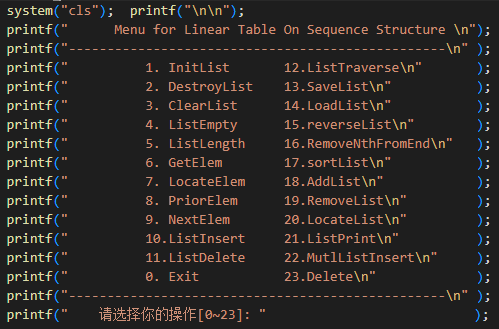
\includegraphics[scale=0.60]{images/1.png}
		\caption{菜单设计代码}
		\label{fig1-1}
	\end{center}
\end{figure}


\subsection{系统实现}
下列函数操作的前提是链表存在,故在每个函数的开始都增添了判空的条件语句,当链表的头结点为空时,返回INFEASIBLE,直接终止函数。
\subsubsection{基础功能}
\begin{itemize}
	\item 初始化表:函数名称是InitList(L);初始条件是线性表L不存在;操作结果是构造一个空的线性表;

	      因为链表结构体在构建设计时在其中添加了名为next的结构体指针实现结构体单元的关联,但该指针是并未被赋值的,因此链表的初始化的一个重要步骤就在于使用malloc
	      函数给结构体指针赋值指向固定空间大小的地址,初始化表即是创建一个头结点,但值得注意的是为保证程序的稳定,在创建完头结点后有必要给头结点的next指针赋空值。
	\item 销毁表:函数名称是DestroyList(L);初始条件是线性表L已存在;操作结果是销毁线性表L;

	      在对链表的销毁中,我们必须知道,不能直接把头结点赋为空值而作为销毁链表的程序运行结果,在链表创建的过程中,每个结点的创建都需要使用malloc函数分配空间,因
	      此倘若程序终止运行,在程序运行的过程中,这些分配的空间是会一直占用的,如若只是单纯地清空头结点,那么这些表面上失去索引而消失的链表结点实际上仍会占用系统空
	      间,如果又在此之上有不断创建链表,程序的运行空间会越来越大,最终导致的结果可能会是内存溢出而导致程序崩溃。

	      因此,为了避免这种错误,我们在销毁链表时需要对链表中的每一个结点进行清空,我们的清空过程会使用free函数,该函数可以释放由 malloc()、calloc()、realloc()
	      等函数申请的内存空间,可以及时释放占用的空间,使程序占用的空间于一个平稳的状态,有效提高程序的稳定性。

	      清除的过程采用while循环直到出现空指针,在清空所有结点后,我们需要把头指针L赋值为空,至此才算真正完成对链表的销毁。
	\item 清空表:函数名称是ClearList(L);初始条件是线性表L已存在;操作结果是将L重置为空表;

	      与上一个函数销毁表唯一的区别仅在于是否对头结点进行处理,销毁的意思即为是整个表彻底消失,而清空是在保证表存在的前提之下实现对表全部内容的清空,而表存在的
	      前提就是头结点的存在与否,所以该函数对销毁表函数进行改进,清空从头结点的next结点开始清空,且循环结束后的赋值改为对头结点的next指针赋空值。
	\item 判定空表:函数名称是ListEmpty(L);初始条件是线性表L已存在;操作结果是若L为空表则返回TRUE,否则返回FALSE;

	      空表的定义即为头结点存在而表中没有任何内容即没有任何子结点,因此除开判断头结点是否为空之后,仅需要判断头结点的next指针是否为空即可。
	\item 求表长:函数名称是ListLength(L);初始条件是线性表已存在;操作结果是返回L中数据元素的个数;

	      判断链表的长度实际上就是对链表进行一次全遍历,没历经一个子结点就对创建的一个int类型初值为零的length变量进行加运算,当while循环跳出即遇到指针时,则链表
	      全遍历完毕,这时再把length作为返回值返回即可。
	\item 获得元素:函数名称是GetElem(L,i,e);初始条件是线性表已存在,1≤i≤ListLength(L);操作结果是用e返回L中第i个数据元素的值;

	      因为函数参数i已经给定范围,所以我们可以直接对数据进行处理,引入一个int型变量count记录当前链表遍历的位置,当count==i时即可跳出循环。

	      为了判断要查找的该元素是否存在设置了如下判断条件,在程序末尾判断结构体指针是否为null值,如果为空值,则说明while循环一直遍历到表尾而仍未跳出循环,即没有
	      找到所需元素,这时返回ERROR。若不为空,则说明找到目标元素,把目标元素的值赋给e,返回OK,即可完成对该功能的需求。
	\item 查找元素:函数名称是LocateElem(L,e,compare());初始条件是线性表已存在;操作结果是返回L中第1个与e满足关系compare()关系的数据元素的位序,若这样
	      的数据元素不存在,则返回值为0。

	      LocateElem函数和GetElem函数可是说是具备着几乎一模一样的程序架构,不同之处在于函数返回值的不同,GetElem最终会返回e的值,而LocteElem返回的是目标元素在
	      链表的物理位置,LocateElem函数在while循环里加了一个if判断语句,当遇到第一个满足compare()关系的元素就直接return position给主函数。在本次实验中,compare
	      ()关系即为==等价关系。
	\item 获得前驱:函数名称是PriorElem(L,cur\_e,pre\_e);初始条件是线性表L已存在;操作结果是若cur\_e是L的数据元素,且不是第一个,则用pre\_e返回它的前驱,否
	      则操作失败,pre\_e无定义。

	      因为链表时顺序遍历的,为了保证能获取到元素的前驱,所以采取使用两个结构体指针,一个为快指针,初值为L->next->next,另一个为慢指针,初值为L->next,当快指针
	      遇到目标元素是即可给pre赋上慢指针的值。

	      在此需要特殊处理的是链表的首节点的情况,因为首节点不存在前驱,为此在函数开头判断如果慢指针的指针域为空,则直接返回ERROR。
	\item 获得后继:函数名称是NextElem(L,cur\_e,next\_e);初始条件是线性表L已存在;操作结果是若cur\_e是L的数据元素,且不是最后一个,则用next\_e返回它的后继,
	      否则操作失败,next\_e无定义。

	      与前面的获取前驱的函数思路相同,但是由于链表的顺序遍历特性,因此相较于获取前驱,获取后驱不需要设置多个指针,在处理特殊情况是也不需要加以特殊的判断语句,只
	      需对while语句的判断条件略加改进,由head!=NULL改为head->next!=NULL,以此完成对核心代码的设计。
	\item 插入元素:函数名称是ListInsert(L,i,e);初始条件是线性表L已存在,1≤i≤ListLength(L)+1;操作结果是在L的第i个位置之前插入新的数据元素e。

	      结合之前的获取前驱函数的思想,设置快慢两个指针,当快指针找寻到目标元素,那么就新创建一个结点作为慢指针的后驱,而新结点的后驱也赋值为快指针指向的目标元素,
	      以此完成对元素的插入。

	      这样的做法需要注意的地方是:基于循环结束的条件fast != NULL,当链表为空表且插入位置为开头时,我们需要进行单独的判断即处理,因为此时fast的值为空值,不会进行
	      while循环;同理的是,当插入位置在表尾时,fast的值同样为空值,这时,程序会跳出while循环,也不会执行插入操作,也需要在while里面加上单独的特殊判断语句,当插入
	      位置为队尾是就直接执行操作。
	      \begin{figure}[htbp]
		      \centering
		      \begin{minipage}{0.7\linewidth}
			      \centering
			      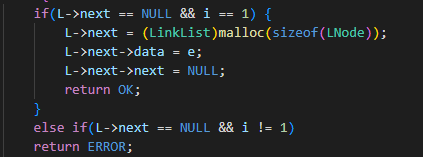
\includegraphics[width=0.9\linewidth]{images/pic-2.png}
		      \end{minipage}

		      \begin{minipage}{0.7\linewidth}
			      \centering
			      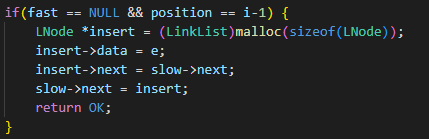
\includegraphics[width=0.9\linewidth]{images/pic-3.png}
		      \end{minipage}
		      \caption{fast指针为空的特殊处理}
		      \label{fig1-2}
	      \end{figure}
	\item 删除元素:函数名称是ListDelete(L,i,e);初始条件是链表L已存在且非空,1≤i≤ListLength(L);操作结果:删除L的第i个数据元素,用e返回其值。

	      运用类似的思维方式,初始化一个遍历指针,然后再定义一个前置指针用于保存的遍历指针指向结点的上一个结点,在遍历指针遍历到目标函数时,采取free函数清空目标结点
	      同时将前置指针指向结点的next指针指向目标结点的下一结点,以此完成对结点的删除。
	\item 遍历表:函数名称是ListTraverse(L,visit()),初始条件是链表L已存在;操作结果是依次对L的每个数据元素调用函数visit()。

	      遍历的表的思想在上述几乎绝大多数函数中得以呈现,遍历均体现出链表的线性结构,在此就不加以过多叙述。进一步健全函数,在开头即可判断链表是否为空,如果为空,直接
	      输出信息告诉使用者并终止函数即可。
\end{itemize}
\subsubsection{附加功能}
\begin{itemize}
	\item 链表翻转:函数名称是reverseList(L),初始条件是线性表L已存在;操作结果是将L翻转;

	      整体上的思路在于是原链表的第一个结点以此后移,每次后移一位就把原位的结点放置到L->next处即作为头结点,具体难点在于如何把后一结点移动到头结点位置。
	      \begin{figure}[htb]
		      \begin{center}
			      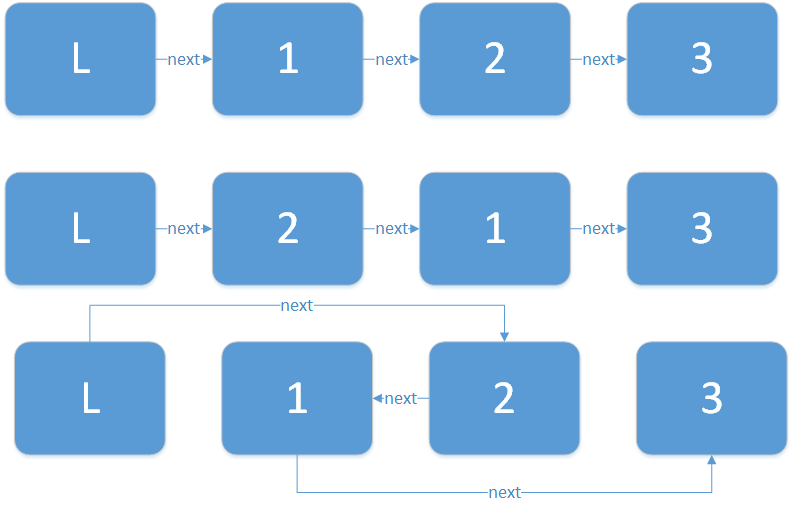
\includegraphics[scale=0.50]{images/pic-4.png}
			      \caption{翻转链表的大致思路}
			      \label{fig1-3}
		      \end{center}
	      \end{figure}
	      算法采取首插法,即每次在首部插入元素以此实现倒序,如图以一个长度为3的链表为例,辅助我们理解结点的移动,本质上就是改变结点的next指针的指向,为了实现这样的设想,我们现需要定义一个temp结构体指针,该指针指向
	      原始链表的头结点head的下一结点,即temp = head->next,head的指向在之后的函数运行过程中一直没有发生改变,即一直指向图中值为1的结点,temp当前指向值为2的结点
	      然后head的next指针指向temp的next指向的结点,即图中值为3的结点,再让temp的next指针指向L的next指向的结点即head结点,最后让L的next指针指向temp即可完成结点
	      的移位,在后续结点的插入过程采取同样的方法,当初始链表的第一个结点移动到链表尾部即head->next为空值时,即可说明链表已经翻转完毕。

	      在程序运行过程中,head的指向保持不变,而temp也始终指向head的next指向的结点,但是head的next指针的指向是在不断变化的,每次的操作实际上就是把当前head的next
	      指针指向的结点移位至表首,让L->next指向head->next,以此循环直至跳出循环。
	\item 删除链表的倒数第n个结点:函数名称是RemoveNthFromEnd(L,n); 初始条件是线性表L已存在且非空, 操作结果是该链表中倒数第n个节点;

	      对于这个功能的实现,我采取了一个投机取巧的办法,运用上一个函数——链表的翻转,在链表翻转过后,对于原链表倒数的结点不就变成正数的结点序号了吗?于是,在函数的最开始
	      先翻转函数,再调用之前写过的删除结点函数删除对应位置的结点即可,在函数结束时再把链表翻转回来即可。

	      但这样在链表体量比较大的时候显然有些欠缺,于是想出另一个做法是,设置两个指针,慢指针比快指针慢n个结点,当快指针遇到链表尾时,慢指针指向的位置即为要删除的位置。
	\item 链表排序:函数名称是sortList(L),初始条件是线性表L已存在;操作结果是将L由小到大排序;

	      对于数组的排序我们都不陌生,我们对于数组排序常用的冒泡排序,对于链表来说同样适用,但需要作出略微的改动,链表交换有两种方式,一种是交换指针域,另一种是交换
	      数据域,本函数采取的是交换数据域,具体思路如下:

	      数据的交换与数组的交换过程类似,都需要一个中间变量temp作为媒介进行交换,难点在于如何让冒泡排序在数组排序中的两个for循环在此得以体现,因为链表是不存在下标访问的
	      ,在此采用的方法是,定义头尾两个指针,头指针每遍历一次链表,尾指针就往前移动一个结点,然后头指针又赋值回头结点的位置,while的结束条件改为头指针的next不等于
	      尾指针,以此实现类似于数组交换第二个for循环的判断条件j < len - i - 1这样的判断效果。
	\item 实现链表的文件形式保存:其中,需要设计文件数据记录格式,以高效保存线性表数据逻辑结构(D,{R})的完整信息;需要设计链表文件保存和加载操作合理模式。

	      文件的存储与读取是相互配套的,文件存储的形式决定文件读取的方式,对于链表这样的简单的线性数据结构,实现文件的存储较为容易,只需满足把每个结点的数据以空格分开的
	      形式用fprintf函数存储在文件中,文件的打开形式是'w',使得每次写入文件都是从头开始写入;在读取文件时,使用fscanf函数,利用它不读取空的特性,结合链表的创建初始化,
	      实现读取每个结点的信息并加以创建,文件的打开形式是'r',保证原文件不会发生改变。

	      在使用文件指针fp时,我们的一个好习惯是在使用fopen函数后应加一个空值判断,以确保文件能正确打开,避免程序错误,同时在程序结尾文件使用完毕后,也应使用fclose函数
	      将文件关闭,避免溢出。
	\item 实现多个线性表管理:设计相应的数据结构管理多个线性表的查找、添加、移除等功能。

	      针对多线性表的管理,实验设计一个新的结构体,其中定义了本实验链表的一个结构体数组,本质上是通过数组存储多个链表以此实现多线性表的管理,针对数组中每个线性表的管理
	      和上述基础功能对单个链表的操作基本一致,不同在于,我们需要实现不同链表的切换,即找寻并切换至目标链表进行管理。

	      在设计过程中每一个链表都有一个name数组对链表进行唯一命名,因此,我们可以采取strcmp函数通过在输入流输入链表的名字实现对不同链表的切换。

	      针对多线性表操作的函数主体架构均和单链表操作的主体架构一直,不同仅在于在函数的开头有判断找寻目的链表的strcmp函数操作,找寻到目标函数则进行后续操作,没有找到目标
	      链表直接返回ERROR。
\end{itemize}
\newpage
\subsection{系统测试}
以下测试数据以及结果均来自与educoder平台以及本机终端,保证数据的精确性以及可靠性、真实性。
\begin{itemize}
	\item InitList测试:\\
	      正常测试:0即创建一个空的头结点指针并传入函数;\\
	      异常测试:1即在主函数中先创建一个非空链表然后把该链表传入函数;
	      \begin{figure}[htbp]
		      \centering
		      \begin{minipage}{0.9\linewidth}
			      \centering
			      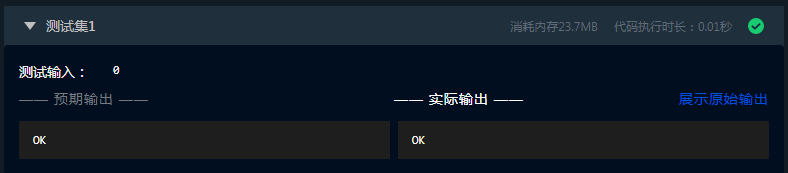
\includegraphics[width=0.9\linewidth]{images/text-1.png}
		      \end{minipage}
		      \begin{minipage}{0.9\linewidth}
			      \centering
			      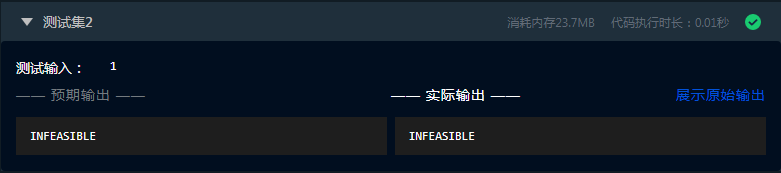
\includegraphics[width=0.9\linewidth]{images/text-2.png}
		      \end{minipage}
		      \caption{InitList函数测试}
		      \label{fig1-4}
	      \end{figure}
	\item DestroyList测试:\\
	      正常测试:输入数据并创建好一个非空链表后,传入函数,并在主函数中判断链表是否结点均清空,成功返回输出OK;\\
	      异常测试:传入一个不存在链表,返回并输出INFEASIBLE;
	      \begin{figure}[htbp]
		      \centering
		      \begin{minipage}{0.9\linewidth}
			      \centering
			      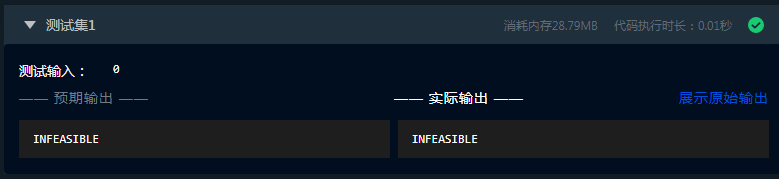
\includegraphics[width=0.9\linewidth]{images/text-3.png}
		      \end{minipage}
		      \begin{minipage}{0.9\linewidth}
			      \centering
			      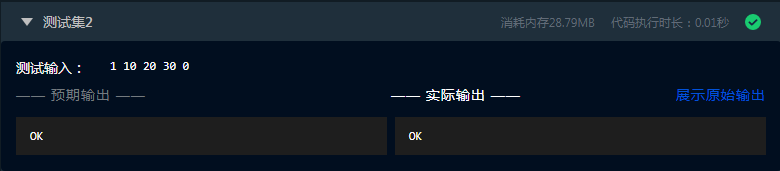
\includegraphics[width=0.9\linewidth]{images/text-4.png}
		      \end{minipage}
		      \caption{DestroyList函数测试}
		      \label{fig1-5}
	      \end{figure}
	\item ClearList测试:\\
	      正常测试:输入数据并创建好一个非空链表后,传入函数,并在主函数中判断除头结点外链表是否结点均清空,即是否为空链表,成功则输出OK;\\
	      异常测试:传入一个不存在链表,返回并输出INFEASIBLE;
	      \begin{figure}[htbp]
		      \centering
		      \begin{minipage}{0.9\linewidth}
			      \centering
			      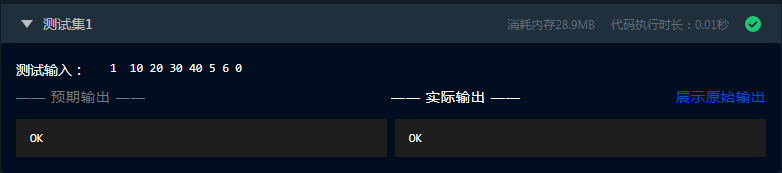
\includegraphics[width=0.9\linewidth]{images/text-5.png}
		      \end{minipage}
		      \begin{minipage}{0.9\linewidth}
			      \centering
			      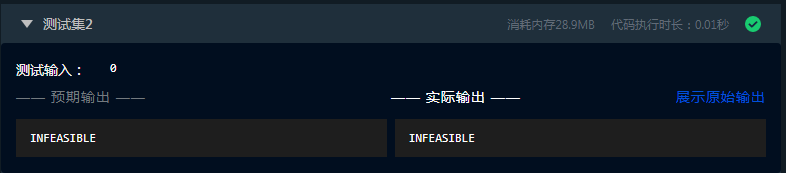
\includegraphics[width=0.9\linewidth]{images/text-6.png}
		      \end{minipage}
		      \caption{ClearList函数测试}
		      \label{fig1-6}
	      \end{figure}
	\item ListEmpty测试:\\
	      正常测试:创建一个非空链表后传入函数,返回FALSE;创建空链表后传入函数,返回TRUE;\\
	      异常测试:传入一个不存在链表,返回INFEASIBLE;
	      \begin{figure}[htbp]
		      \centering
		      \begin{minipage}{0.9\linewidth}
			      \centering
			      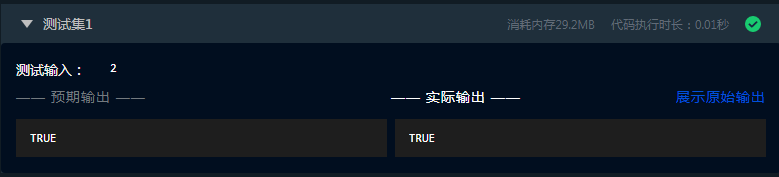
\includegraphics[width=0.9\linewidth]{images/text-7.png}
		      \end{minipage}
		      \begin{minipage}{0.9\linewidth}
			      \centering
			      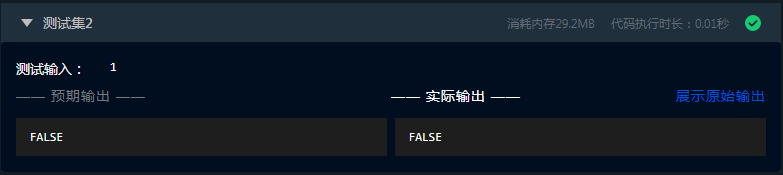
\includegraphics[width=0.9\linewidth]{images/text-8.png}
		      \end{minipage}
		      \begin{minipage}{0.9\linewidth}
			      \centering
			      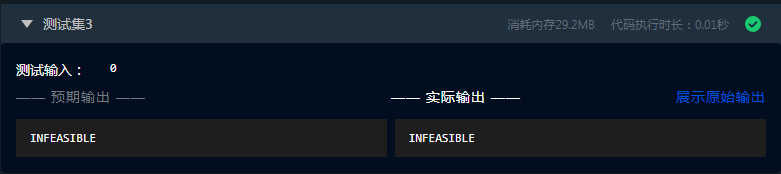
\includegraphics[width=0.9\linewidth]{images/text-9.png}
		      \end{minipage}
		      \caption{ListEmpty函数测试}
		      \label{fig1-7}
	      \end{figure}
	\item ListLength测试:\\
	      正常测试:创建一个长度为5的链表,传入函数,函数返回值为5;\\
	      异常测试:传入一个不存在链表,返回INFEASIBLE;
	      \newpage
	      \begin{figure}[htbp]
		      \centering
		      \begin{minipage}{0.9\linewidth}
			      \centering
			      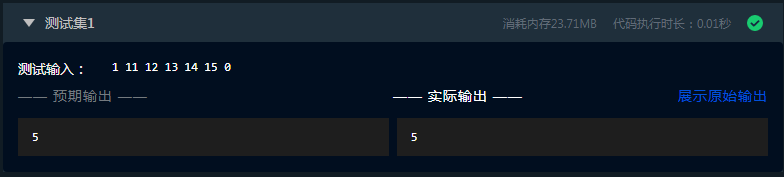
\includegraphics[width=0.9\linewidth]{images/text-10.png}
		      \end{minipage}
		      \begin{minipage}{0.9\linewidth}
			      \centering
			      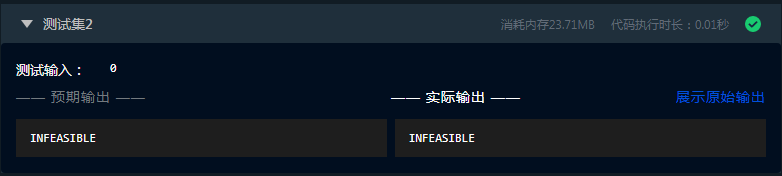
\includegraphics[width=0.9\linewidth]{images/text-11.png}
		      \end{minipage}
		      \caption{ListLength函数测试}
		      \label{fig1-8}
	      \end{figure}
	\item GetElem测试:\\
	      正常测试:创建一个长度为5的非空链表后传入函数,在函数长度范围内查询元素,返回OK;\\
	      异常测试:创建一个长度为5的非空链表后传入函数,在函数长度范围之外查询元素如输入的查询位置为0或者8,返回ERROR;传入一个不存在链表,返回INFEASIBLE;
	      \begin{figure}[htbp]
		      \centering
		      \begin{minipage}{0.9\linewidth}
			      \centering
			      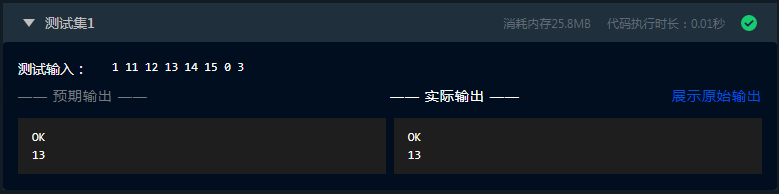
\includegraphics[width=0.9\linewidth]{images/test-12.png}
		      \end{minipage}
		      \begin{minipage}{0.9\linewidth}
			      \centering
			      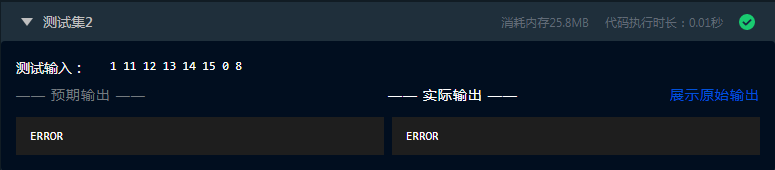
\includegraphics[width=0.9\linewidth]{images/test-13.png}
		      \end{minipage}
		      \begin{minipage}{0.9\linewidth}
			      \centering
			      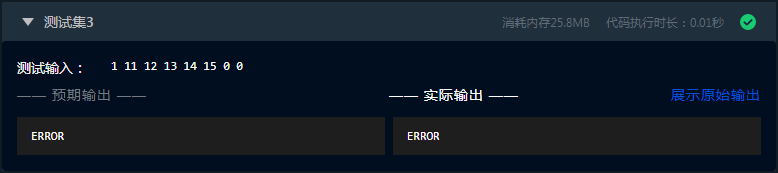
\includegraphics[width=0.9\linewidth]{images/test-14.png}
		      \end{minipage}
		      \begin{minipage}{0.9\linewidth}
			      \centering
			      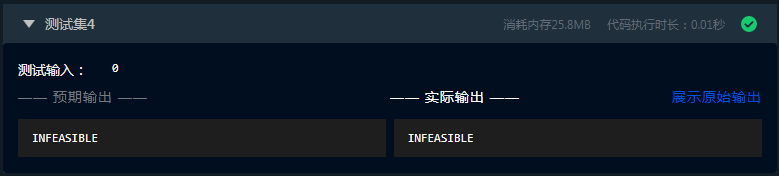
\includegraphics[width=0.9\linewidth]{images/test-15.png}
		      \end{minipage}
		      \caption{GetElem函数测试}
		      \label{fig1-9}
	      \end{figure}
	\item LocateElem测试:\\正常测试:创建一个数据为11 12 13 14 15长度为5的链表,查询14的位置,返回4;\\异常测试:传入同样链表查询不存在的元素18的位置,返回ERROR;传入一个不存在链表,返回INFEASIBLE;
	      \begin{figure}[htbp]
		      \centering
		      \begin{minipage}{0.9\linewidth}
			      \centering
			      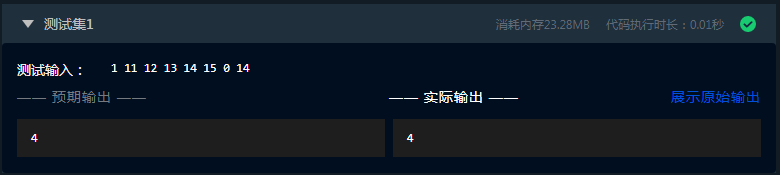
\includegraphics[width=0.9\linewidth]{images/test-16.png}
		      \end{minipage}
		      \begin{minipage}{0.9\linewidth}
			      \centering
			      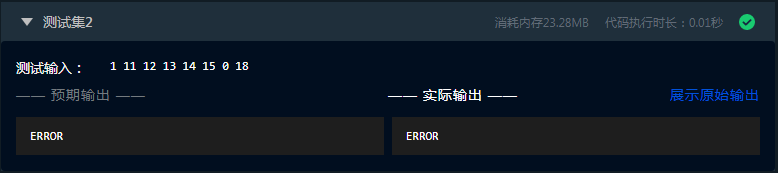
\includegraphics[width=0.9\linewidth]{images/test-17.png}
		      \end{minipage}
		      \begin{minipage}{0.9\linewidth}
			      \centering
			      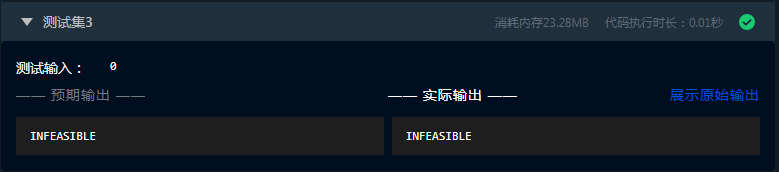
\includegraphics[width=0.9\linewidth]{images/test-18.png}
		      \end{minipage}
		      \caption{LocateElem函数测试}
		      \label{fig1-10}
	      \end{figure}
	\item PriorElem测试:\\正常测试:创建一个数据为11 12 13 14 15长度为5的链表,查询14的前驱,返回13,输出OK;\\异常测试:查询11的前驱,返回ERROR;查询不存在元素18的前驱,返回ERROR;传入一个不存在链表,返回INFEASIBLE;
	      \begin{figure}[htbp]
		      \centering
		      \begin{minipage}{0.9\linewidth}
			      \centering
			      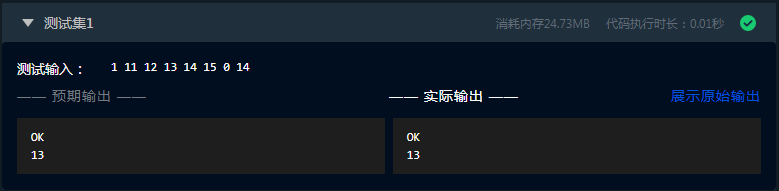
\includegraphics[width=0.9\linewidth]{images/test-19.png}
		      \end{minipage}
		      \begin{minipage}{0.9\linewidth}
			      \centering
			      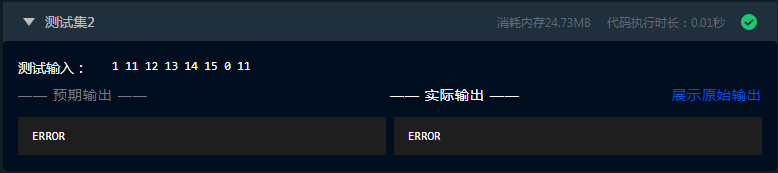
\includegraphics[width=0.9\linewidth]{images/test-20.png}
		      \end{minipage}
	      \end{figure}
	      \newpage
	      \begin{figure}[htbp]
		      \centering
		      \begin{minipage}{0.9\linewidth}
			      \centering
			      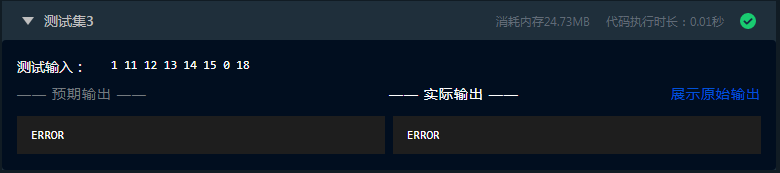
\includegraphics[width=0.9\linewidth]{images/test-21.png}
		      \end{minipage}
		      \begin{minipage}{0.9\linewidth}
			      \centering
			      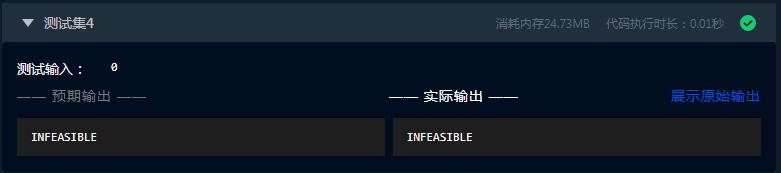
\includegraphics[width=0.9\linewidth]{images/test-22.png}
		      \end{minipage}
		      \caption{PriorElem函数测试}
		      \label{fig1-11}
	      \end{figure}
	\item NextElem测试:\\正常测试:创建一个数据为11 12 13 14 15长度为5的链表,查询14的后驱,返回15,输出OK;\\异常测试:查询15的后驱,返回ERROR;查询不存在元素18的后驱,返回ERROR;传入一个不存在链表,返回INFEASIBLE;
	      \begin{figure}[htbp]
		      \centering
		      \begin{minipage}{0.9\linewidth}
			      \centering
			      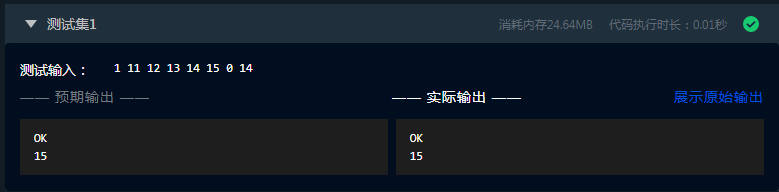
\includegraphics[width=0.9\linewidth]{images/test-23.png}
		      \end{minipage}
		      \begin{minipage}{0.9\linewidth}
			      \centering
			      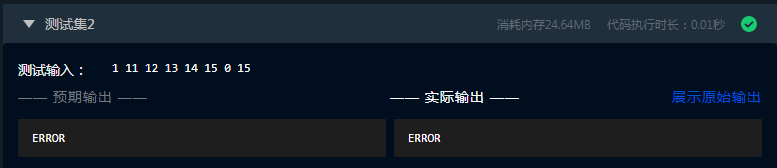
\includegraphics[width=0.9\linewidth]{images/test-24.png}
		      \end{minipage}
		      \begin{minipage}{0.9\linewidth}
			      \centering
			      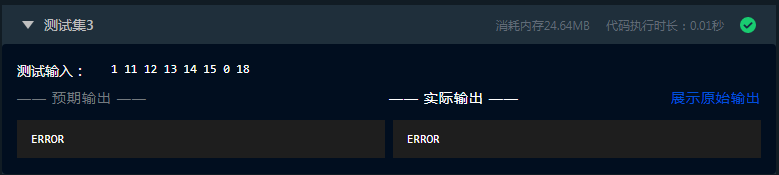
\includegraphics[width=0.9\linewidth]{images/test-25.png}
		      \end{minipage}
		      \begin{minipage}{0.9\linewidth}
			      \centering
			      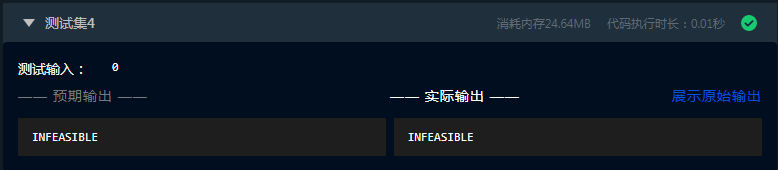
\includegraphics[width=0.9\linewidth]{images/test-26.png}
		      \end{minipage}
		      \caption{NextElem函数测试}
		      \label{fig1-12}
	      \end{figure}
	\item ListInsert测试:\\
	      正常测试:创建一个数据为1 3 5 7 9 2 4 6 8 10的链表,在第五个元素前面插入80,返回OK;\\
	      异常测试:创建一个数据为10 20 30的链表,在第0个和第5个位置插入元素,返回ERROR;传入一个不存在链表,返回INFEASIBLE;\\
	      特殊数据测试:传入正常测试的链表数据,在最大容量元素的后一元素位置前插入,本实验中链表最大容量为10,但可以在第十一个元素的前面插入元素,返回OK;传入一个空链表,在第一个位置前插入,返回OK;
	      \begin{figure}[htbp]
		      \centering
		      \begin{minipage}{0.9\linewidth}
			      \centering
			      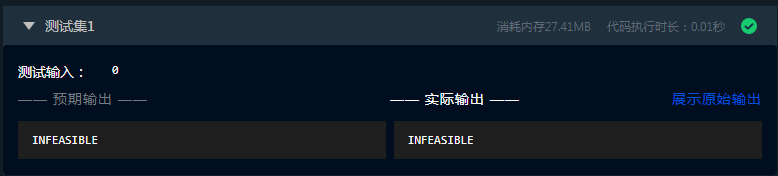
\includegraphics[width=0.9\linewidth]{images/test-27.png}
		      \end{minipage}
		      \begin{minipage}{0.9\linewidth}
			      \centering
			      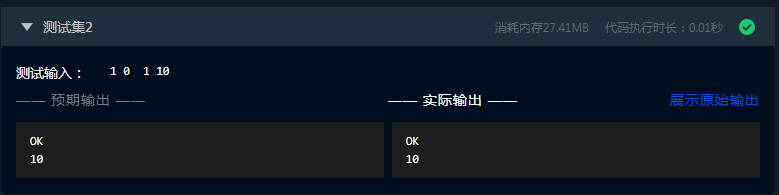
\includegraphics[width=0.9\linewidth]{images/test-28.png}
		      \end{minipage}
		      \begin{minipage}{0.9\linewidth}
			      \centering
			      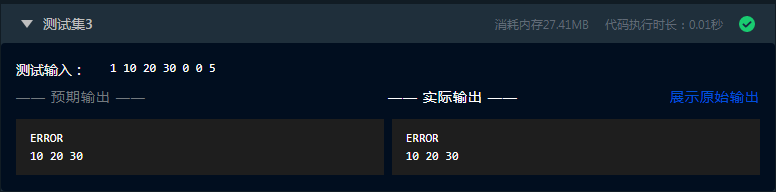
\includegraphics[width=0.9\linewidth]{images/test-29.png}
		      \end{minipage}
		      \begin{minipage}{0.9\linewidth}
			      \centering
			      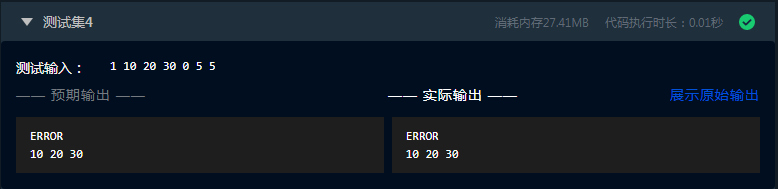
\includegraphics[width=0.9\linewidth]{images/test-30.png}
		      \end{minipage}
		      \begin{minipage}{0.9\linewidth}
			      \centering
			      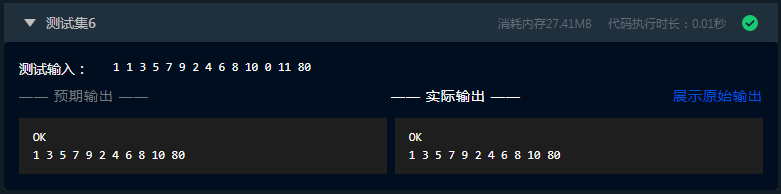
\includegraphics[width=0.9\linewidth]{images/test-31.png}
		      \end{minipage}
		      \caption{ListInsert函数测试}
		      \label{fig1-13}
	      \end{figure}
	\item ListDelete测试:\\
	      正常测试:创建一个数据为11 12 13 14 15的链表,删除3位置的元素返回OK;\\
	      异常测试:同样的链表,删除0位置和6位置的元素,即超出链表长度范围删除,返回ERROR;传入一个不存在链表,返回INFEASIBLE;\\
	      特殊数据测试:表首和表尾数据删除测试,返回OK
	      \begin{figure}[htbp]
		      \centering
		      \begin{minipage}{0.9\linewidth}
			      \centering
			      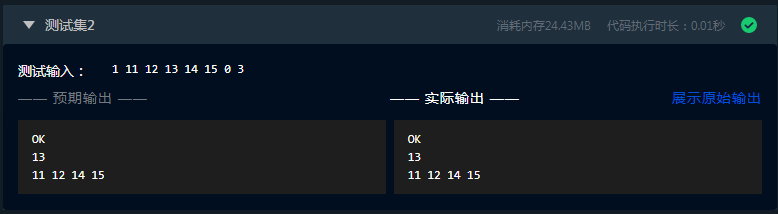
\includegraphics[width=0.9\linewidth]{images/test-33.png}
		      \end{minipage}
		      \begin{minipage}{0.9\linewidth}
			      \centering
			      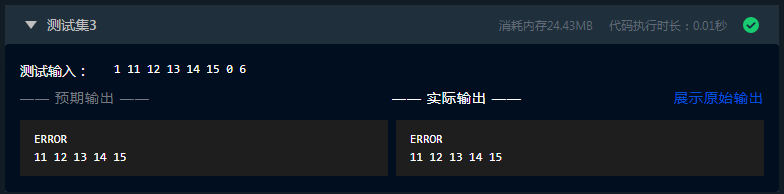
\includegraphics[width=0.9\linewidth]{images/test-34.png}
		      \end{minipage}
		      \begin{minipage}{0.9\linewidth}
			      \centering
			      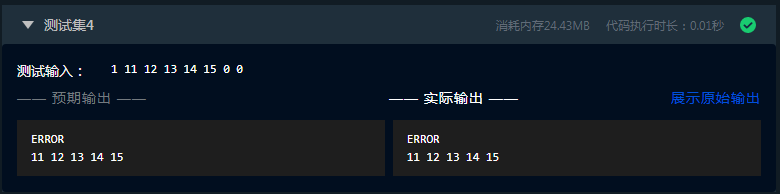
\includegraphics[width=0.9\linewidth]{images/test-35.png}
		      \end{minipage}
		      \begin{minipage}{0.9\linewidth}
			      \centering
			      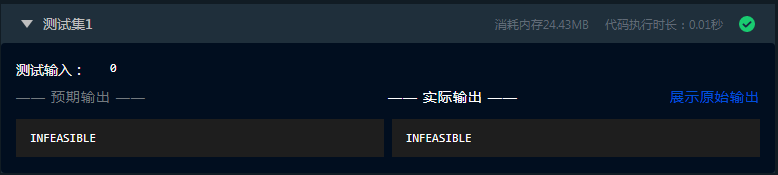
\includegraphics[width=0.9\linewidth]{images/test-32.png}
		      \end{minipage}
		      \begin{minipage}{0.9\linewidth}
			      \centering
			      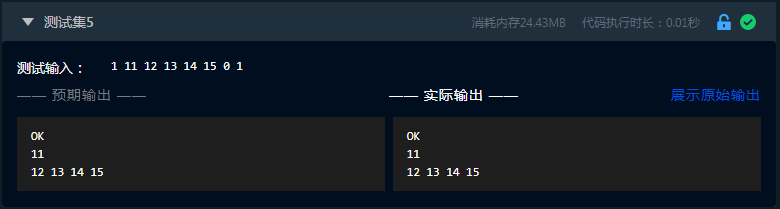
\includegraphics[width=0.9\linewidth]{images/test-36.png}
		      \end{minipage}
	      \end{figure}
	      \newpage
	      \begin{figure}[htbp]
		      \centering
		      \begin{minipage}{0.9\linewidth}
			      \centering
			      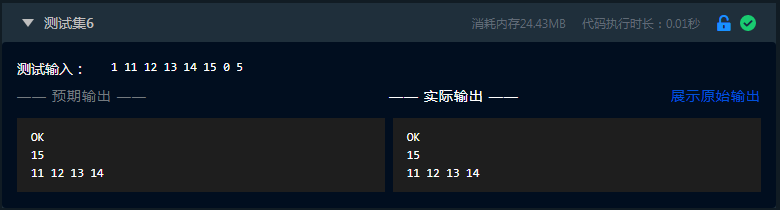
\includegraphics[width=0.9\linewidth]{images/test-37.png}
		      \end{minipage}
		      \caption{ListDelete函数测试}
		      \label{fig1-14}
	      \end{figure}
	\item ListTraverse测试:\\正常测试:遍历输出数据为11 12 13 14 15的链表;\\异常测试:传入一个不存在链表,返回INFEASIBLE;\\特殊数据测试:传入一个空链表,输出该链表为空;
	      \begin{figure}[htbp]
		      \centering
		      \begin{minipage}{0.9\linewidth}
			      \centering
			      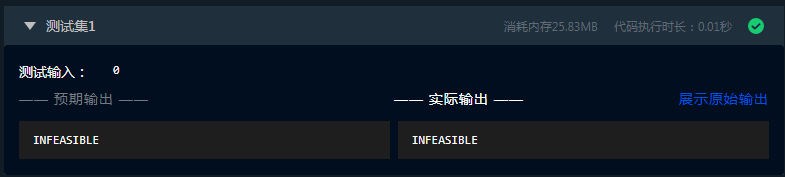
\includegraphics[width=0.9\linewidth]{images/test-38.png}
		      \end{minipage}
		      \begin{minipage}{0.9\linewidth}
			      \centering
			      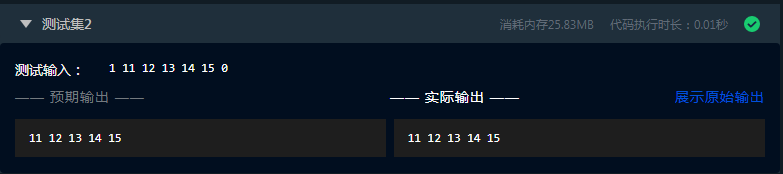
\includegraphics[width=0.9\linewidth]{images/test-39.png}
		      \end{minipage}
		      \begin{minipage}{0.9\linewidth}
			      \centering
			      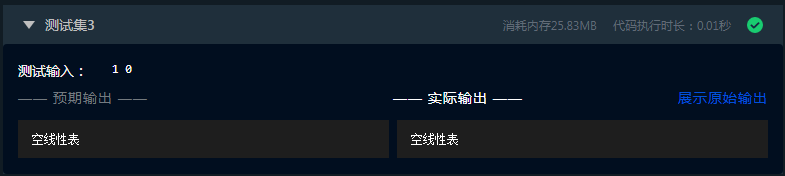
\includegraphics[width=0.9\linewidth]{images/test-40.png}
		      \end{minipage}
		      \caption{ListTraverse函数测试}
		      \label{fig1-15}
	      \end{figure}
	\item reverseList测试:\\正常测试:翻转数据为11 12 13 14 15的链表,并遍历输出;\\异常测试:传入一个不存在链表,返回INFEASIBLE;\\特殊数据测试:传入一个空链表;
	      \newpage
	      \begin{figure}[htbp]
		      \centering
		      \begin{minipage}{0.9\linewidth}
			      \centering
			      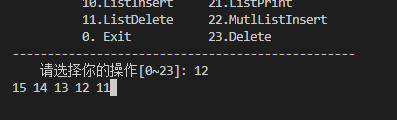
\includegraphics[width=0.9\linewidth]{images/test-41.png}
		      \end{minipage}
		      \begin{minipage}{0.9\linewidth}
			      \centering
			      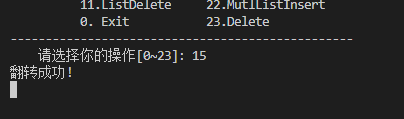
\includegraphics[width=0.9\linewidth]{images/test-42.png}
		      \end{minipage}
		      \begin{minipage}{0.9\linewidth}
			      \centering
			      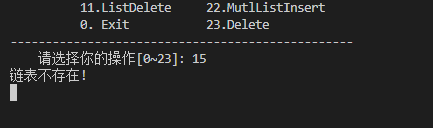
\includegraphics[width=0.9\linewidth]{images/test-43.png}
		      \end{minipage}
		      \caption{reverseList函数测试}
		      \label{fig1-16}
	      \end{figure}
	\item RemoveNthFromEnd测试:\\正常测试:创建一个数据为11 12 13 14 15的链表,删除倒数第二个结点;\\异常测试:传入一个不存在链表,返回INFEASIBLE;
	      \begin{figure}[htbp]
		      \centering
		      \begin{minipage}{0.9\linewidth}
			      \centering
			      
\includegraphics[width=0.9\linewidth]{images/test-44.png}
		      \end{minipage}
	      \end{figure}
	      \newpage
	      \begin{figure}[htbp]
		      \centering
		      \begin{minipage}{0.9\linewidth}
			      \centering
			      \includegraphics[width=0.9\linewidth]{images/test-45.png}
		      \end{minipage}
		      \begin{minipage}{0.9\linewidth}
			      \centering
			      \includegraphics[width=0.9\linewidth]{images/test-46.png}
		      \end{minipage}
		      \caption{RemoveNthFromEnd函数测试}
		      \label{fig1-17}
	      \end{figure}
	\item sortList测试:\\正常测试:创建一个数据为1 3 5 2 4的链表,排序并输出;\\异常测试:传入一个不存在链表,返回INFEASIBLE;
	      \begin{figure}[htbp]
		      \centering
		      \begin{minipage}{0.9\linewidth}
			      \centering
			      \includegraphics[width=0.9\linewidth]{images/test-47.png}
		      \end{minipage}
		      \begin{minipage}{0.9\linewidth}
			      \centering
			      \includegraphics[width=0.9\linewidth]{images/test-48.png}
		      \end{minipage}
		      \begin{minipage}{0.9\linewidth}
			      \centering
			      \includegraphics[width=0.9\linewidth]{images/test-49.png}
		      \end{minipage}
		      \caption{RemoveNthFromEnd函数测试}
		      \label{fig1-18}
	      \end{figure}
	\item SaveList、LoadList测试:\\正常测试:创建一个非空链表后传入函数,存入文件后销毁链表,在重新读取文件创建链表并输出;\\异常测试:传入一个不存在链表,返回INFEASIBLE;
	      \begin{figure}[htbp]
		      \centering
		      \begin{minipage}{0.9\linewidth}
			      \centering
			      \includegraphics[width=0.9\linewidth]{images/test-50.png}
		      \end{minipage}
		      \begin{minipage}{0.9\linewidth}
			      \centering
			      \includegraphics[width=0.9\linewidth]{images/test-51.png}
		      \end{minipage}
		      \caption{SaveList、LoadList函数测试}
		      \label{fig1-19}
	      \end{figure}
	\item 多线性表测试:\\
	      创建名为a,b的两个链表,两个链表的数据均为1 2 3 4 5,对a增添数据6在4和5中间,对b删除数据1;随后销毁表b,再创建一个空表c\\
	      \begin{figure}[htbp]
		      \centering
		      \begin{minipage}{0.9\linewidth}
			      \centering
			      \includegraphics[width=0.9\linewidth]{images/test-52.png}
		      \end{minipage}
		      \begin{minipage}{0.9\linewidth}
			      \centering
			      \includegraphics[width=0.9\linewidth]{images/test-53.png}
		      \end{minipage}
		      \begin{minipage}{0.9\linewidth}
			      \centering
			      \includegraphics[width=0.9\linewidth]{images/test-54.png}
		      \end{minipage}
	      \end{figure}
	      \begin{figure}[htbp]
		      \centering
		      \begin{minipage}{0.9\linewidth}
			      \centering
			      \includegraphics[width=0.9\linewidth]{images/test-55.png}
		      \end{minipage}
		      \caption{SaveList、LoadList函数测试}
		      \label{fig1-20}
	      \end{figure}
\end{itemize}

\subsection{实验小结}

重点说明在实验中取得的实际经验,例如调试中碰到的典型错误等,不要写套话。

在编写ClearList的过程中一开始并不能通过头歌平台的测试,对自己的函数一番审视过后发现,后来加入了L->next = NULL;这个语句后就顺利地通过了测试,在我百思不得其解,后
通过上网查资料才得知,free函数不能使free掉指针指向空,即指针所指向的地址没有发生改变,只是指针指向地址存储的内容均已被情况,因为我们是为了清空链表,L->next依照
定义应该指向空,也避免程序报错,因此,将L->next赋值为空是必要且必须的。

GetElem函数在实验要求中,虽然对i的值做了规范,但难免会出现使用者输错值的情况,为了是程序更加的完善,有必要对不合法的i进行报错,并输出相关信息提示。

PriorElem在编写设计的过程中设置了快慢指针,但是在最初的调试过程中发现,函数对空表进行运行时会导致程序报错退出,使用单步调试后发现,快指针fast指向的是L->next->next,当
L->next为空,即链表为空时,是不存在L->next->next的,因而程序会退出崩溃,这样提示我,在未来程序的编写中应当注意跨度大的指针能否存在的问题。

ListInsert在头歌平台评测时,最初没有通过特殊情况的数据测试,分别是在空表时进行的插入,以及非空表情况下的尾部插入,空表时插入失败的原因和ClearList的问题非常类似,
因为while循环的判断条件为fast != NULL,而表为空表时,fast的值为空,那么这时就不会进入while循环进行插入操作;同理,尾部插入失败也是一样的道理,while循环的末尾,
fast = fast->next,当fast为表尾时,判断就直接跳出,假若此时插入位置也刚好在表尾,因此跳出循环而不会进行插入操作,因此,对于这两种情况,在函数里都做了特殊判断。

在编写获得前驱这些需要获取目标结点的上一结点的函数时,我都运用了两个指针一快一慢来确保能够获取前一个指针,但其实完全没有必要这么麻烦,要求获取第i个元素的前驱,
那么我直接定位获取第i-1位的元素不就行了吗?这样的做法就不需要定义两个指针,而且在表首没有前驱的问题上也不需要特殊判断,只要i-1大于等于0那么就即可插入,这是我的程序可以有所改进的地方。


\newpage

\section{基于二叉链表的二叉树实现}
本章将实现新的数据类型结构——二叉树,并实现和探讨二叉链表结构之下的非线性结构的基础功能的实现及其设计原理。

\subsection{问题描述}
\begin{itemize}
	\item 加深对二叉树的概念、基本运算的理解;
	\item 熟练掌握二叉树的逻辑结构与物理结构的关系;
	\item 以二叉链表作为物理结构,熟练掌握二叉树基本运算的实现。
\end{itemize}

\subsection{系统设计}
基于二叉树的定义:二叉树是一种每个结点至多只有两个子树(即二叉树的每个结点的度不大于2),并且二叉树的子树有左右之分,其次序不能任意颠倒。二叉树同时又需具备存储数据的能力
,于是设计如图所示结构体:
\begin{center}
	\noindent{基本结构设计代码}
	\label{lst-2}
\end{center}
\begin{lstlisting}
typedef int status;
typedef int KeyType; 
typedef struct {
	KeyType  key;
	char others[20];
} TElemType; //二叉树结点类型定义

typedef struct BiTNode{  //二叉链表结点的定义
	TElemType  data;
	struct BiTNode *lchild,*rchild;
} BiTNode, *BiTree;
\end{lstlisting}
二叉树的结构体中包含名为data的结点类型结构体变量,同时还包含左右子树的结构体指针,后续树的创建过程中分别指向本结点的左右子结点,完成树结点间的连接。

结点类型结构体定义为int类型的关键词,这是值唯一的数据,保证结点数据不会出现重复。char类型的others数组则就是用来存储数据的。
为了实现后续的多二叉树管理,设计如下多二叉树管理的结构体:
\begin{center}
	\noindent{多二叉树结构设计代码}
	\label{lst-3}
\end{center}
\begin{lstlisting}
typedef struct{  //多二叉树的管理表定义
struct { 
	char name[30];
	BiTree T;	
} elem[10];
int length;
int listsize;
}LISTS;
\end{lstlisting}
结构原理同链表操作中的多链表管理类似,在此不再加以解释。

在程序实际运行的可视化简易菜单上,采用printf的简易方式打印出菜单并设计while循环实现程序的多次操作,并根据输入数字对用switch函数中的不同具体功能选项。
\begin{figure}[htb]
	\begin{center}
		\includegraphics[scale=0.50]{images/menu.png}
		\caption{二叉树菜单代码设计}
		\label{fig2-1}
	\end{center}
\end{figure}
\subsection{系统实现}
下列函数操作的前提是链表存在,故在每个函数的开始都增添了判空的条件语句,当链表的头结点为空时,直接终止函数。
\subsubsection{基础功能}
\begin{itemize}
	\item 创建二叉树:函数名称是CreateBiTree(T,definition);初始条件是definition 给出二叉树T的定义,如带空子树的二叉树前序遍历序列、或前序+中序、或后序+中序;操作结果是按definition构造二叉树T;\\
	      definition在当前函数以及后续几乎所有函数中都是遵循这样的输入原则,如:1 a 2 b 0 null  0 null 3 c 4 d  0 null  0 null 5 e  0 null  0 null -1 null

	      definition会按照先序遍历的顺序给出所有包括空结点在内的结点,在此基础之上的树的创建的函数思路如下:

	      因为definition采用先序存储方式,所以函数也采取先序构建树,由先序的特性我们可以知道,任何一个结点的右子树的创建一定是在其左子树已经构建完的基础之上,因此一棵树一定会
	      先创建完左子树再开始创建右子树,创建过程如图:
	      \begin{figure}[htb]
		      \begin{center}
			      \includegraphics[scale=0.50]{images/pic-5.png}
			      \caption{二叉树创建流程示意图}
			      \label{fig2-2}
		      \end{center}
	      \end{figure}
	      基于这种创建方式,避免不了回溯的问题,在非递归的算法之下,本函数采用使用栈来进行回退,当一条分支不能再创建左子树时,即图中第一步时,那么就开始给最末端的树叶
	      创建右子树,树叶创建好后,如果右子树也为空,那么就会开始回退到上一个根节点即图中的a结点,此时有一个问题显而易见,我们如何判断栈中回溯的结点是否已经创建了左子树呢?
	      这个时候通过引入一个与栈同步的标记数组,初值为0,把栈中已经创建左子树的结点的位置在数组中标记为一,回退时通过判断数组值是否为1来决定回溯结点是创建左子树还是创建右子树。

	      在函数的while循环中把创建左子树放在前面,把创建右子树放在后面,而且创建右子树的函数功能增添一个判断语句来判断是否应该启动,在创建完一个结点的左右结点后,我们要记得进行
	      退栈操作,同时把标记数组对应位置初始化为0。

	      针对特殊情况的数据处理,例如树为空的情况,本函数在函数开头就加以判断,若为空,则直接返回OK,表示空树创建完毕。
	\item 销毁二叉树:函数名称是DestroyBiTree(T);初始条件是二叉树T已存在;操作结果是销毁二叉树T;

	      清空二叉树:函数名称是ClearBiTree (T);初始条件是二叉树T存在;操作结果是将二叉树T清空;

	      这里将清空与销毁一同叙述,与链表的销毁清空类似的是,这个过程都需要全部遍历一遍树的所有结点,并使用free函数清空遍历过的结点。清空与销毁的不同又在于是否对头结点进行
	      free函数操作,清空不对头结点操作,而销毁是会对头结点进行清除操作。

	      本函数采用非递归后序遍历的方式实现树的遍历的。
	\item 判定空二叉树:函数名称是BiTreeEmpty(T);初始条件是二叉树T存在;操作结果是若T为空二叉树则返回TRUE,否则返回FALSE;

	      仅需要判断头结点指针是否为空即可,T指向NULL则返回TRUE,不为空则返回FALSE。
	\item 求二叉树深度:函数名称是BiTreeDepth(T);初始条件是二叉树T存在;操作结果是返回T的深度;

	      该函数实现的核心思想是,遍历到一个层数最大的一个分支,本函数的思想是,在非递归的算法中,遍历为了实现回退需要用到栈,而栈所能达到的最大高度是和树的层数有关的,
	      在本函数采取的后序非递归遍历中,栈的栈顶位置就等于当前所处的层数,所以新定义一个max变量用于保存在遍历过程中栈顶位置的最大值,在遍历完所有结点后,返回的max值
	      就即为二叉树的深度。
	\item 查找结点:函数名称是LocateNode(T,e);初始条件是二叉树T已存在,e是和T中结点关键字类型相同的给定值;操作结果是返回查找到的结点指针,如无关键字为e的结点,返回NULL;\\
	      该函数的返回值为指针类型,在查找过程中基于关键字的唯一性,所以通过比较语句发现关键字相同的结点即可把当前遍历的结点作为返回值返回,在循环外返回空指针,表示遍历过程如果没有
	      正常return,就说明树中没有对应的结点,返回空指针表示查找失败。
	\item 结点赋值:函数名称是Assign(T,e,value);初始条件是二叉树T已存在,e是和T中结点关键字类型相同的给定值;操作结果是关键字为e的结点赋值为value;\\
	      该函数的核心算法以及思想与上面的查找结点函数相同,都是在遍历过程中找到对应的结点,但是我们值得注意的地方是,我们重新赋完值后,仍需保证树中不会存在重复的关键字
	      ,即须保证关键字的唯一性,所以我们不能在遍历到目标结点就直接完成赋值操作并返回,而是先把目标结点的信息先保存下来,在遍历完所有结点后,再进行赋值操作。函数定义一个
	      标记数组,初值为0,当关键字出现过一次时就把标记值改为1,在遍历完成后,我们需要判断标记数组中重新赋值的关键字的标记值是否为0,为0说明该关键字没出现过,为1则说明
	      该关键字已经存在,不能进行重新赋值操作,返回ERROR。
	\item 获得兄弟结点:函数名称是GetSibling(T,e);初始条件是二叉树T存在,e是和T中结点关键字类型相同的给定值;操作结果是返回关键字为e的结点的(左或右)兄弟结点指针。若关键字为e的结点无兄弟,则返回NULL;\\
	      函数的基本思路是:运用后序遍历找到目标子结点,然后回溯到该结点的父节点,然后返回该父节点的另一子节点。\\
	      思路很简单,难点在于如何回溯到父节点,由后序遍历的特性我们知道,后序遍历是先遍历两个子节点再遍历父节点的,因此在非递归算法中,一个结点在栈中位置的下一个结点
	      必然为它的父节点,后序每次都是遍历栈顶元素,因此,目标结点的父节点就即为Stack[top-2]保存的结点,获得父节点后再通过if语句判断目标结点是父节点的左子树或者右子树,
	      依据结果返回父节点的右子树或者左子树。
	\item 插入结点:函数名称是InsertNode(T,e,LR,c);初始条件是二叉树T存在,e是和T中结点关键字类型相同的给定值,LR为0或1,c是待插入结点;操作结果是根据LR为0或者1,插入结点c到T中,作为关键字为e的结点的左或右孩子结点,结点e的原有左子树或右子树则为结点c的右子树;
	      特殊情况,c插入作为根结点?可以考虑LR为-1时,作为根结点插入,原根结点作为c的右子树。\\
	      该函数要实现的功能较多,首先考虑当LR为-1的时候,操作相较于其他插入有所不同,因而单独拎出来进行操作,依据功能要求将插入根节点作为插入结点的右子树即可。\\
	      插入结点的算法是结合了结点查找和结点赋值两个函数的算法思想,首先需要查找到插入的位置,即查找到目标结点,但是同样的,为了保证插入结点之后仍能保证关键字的唯一性,
	      我们需要保存目标结点的位置,然后让程序继续遍历完整个树,在此过程中用标记数组记录遇到的每一个关键字,并修改标记值为1。\\
	      在遍历完成后,判断关键字是否重复,若重复则返回ERROR,若唯一,那么再依据LR的值完成相应操作即可,赋值的过程较为简单,在此就不加以过多叙述。
	\item 删除结点:函数名称是DeleteNode(T,e);初始条件是二叉树T存在,e是和T中结点关键字类型相同的给定值。操作结果是删除T中关键字为e的结点;同时,如果关键字为e的结点度为0,删除即可;如关键字为e的结点度为1,用关键字为e的结点孩子代替被删除的e位置;如关键字为e的结点度为2,用e的左孩子代替被删除的e位置,e的右子树作为e的左子树中最右结点的右子树;\\
	      该函数的主体思路与上面的函数大致相同,无非就是遍历到目标位置再进行操作,本函数的复杂之处在于对于删除结点不同度的要进行不同操作。\\
	      度为0时的操作是最简单的,无需考虑删除过后子节点的后续处理工作,直接free掉该结点即可。\\
	      度为1时,首先先判断该结点是其父节点的左子树还是右子树,这里运用到获取兄弟结点的思想获取父节点,判断完左右子树后,再让父节点的左右指针指向删除结点的子节点即可。\\
	      度为2时,与度为1时的操作思路大致相同,只不过需要用一个while循环获取e左子树的最右子树的位置,具体操作过程和度为1的情况大致相同,在此略过。\\
	      需要特殊处理的是对头结点的删除操作,因为对头结点的操作会改变T的指向,而非头结点的删除操作并不会改变T的指向,因此需要单独对这种情况进行特殊处理,处理的过程和非
	      头结点的操作流程是一致的,只是操作完后需要对T重新赋值。
	\item 前序遍历:函数名称是PreOrderTraverse(T,Visit);初始条件是二叉树T存在,Visit是一个函数指针的形参(可使用该函数对结点操作);操作结果:先序遍历,对每个结点调用函数Visit一次且一次,一旦调用失败,则操作失败。\\
	      实现思想:借助栈,对于根节点,先将当前节点压入栈中,然后遍历的时候弹出栈中的一个元素,输出,当该节点的右节点不为空时,将节点压入栈,当左节点不为空时,将左节点压入栈,前序遍历是根左右但是栈的数据结构时先入后出,先访问到左
	      节点,需要将右节点先压入栈中。继续循环,弹出栈顶元素,输出,将右节点和左节点压入栈中。
	\item 中序遍历:函数名称是InOrderTraverse(T,Visit);初始条件是二叉树T存在,Visit是一个函数指针的形参(可使用该函数对结点操作);操作结果是中序遍历t,对每个结点调用函数Visit一次且一次,一旦调用失败,则操作失败;\\
	      实现思想:在第二次经过结点的时候才去访问结点数据,要一直去寻找结点的左子树,访问完左子树在返回结点并获取结点数据,然后访问右子树,重复这个过程,也就是说如果当前结点有左子树就要转去左子树,访问完左子树才访问当前结点,
	      这个场景刚好可以使用栈来实现,有左子树则把当前结点入栈,访问完左子树,再出栈并访问结点数据。
	\item 后序遍历:函数名称是PostOrderTraverse(T,Visit);初始条件是二叉树T存在,Visit是一个函数指针的形参(可使用该函数对结点操作);操作结果是后序遍历t,对每个结点调用函数Visit一次且一次,一旦调用失败,则操作失败。\\
	      实现思想:对于任一结点P,将其入栈,然后沿其左子树一直往下搜索,直到搜索到没有左孩子的结点,此时该结点出现在栈顶,但是此时不能将其出栈并访问, 因此其右孩子还为被访问。所以接下来按照相同的规则对其右子树进行相同的处理,当
	      访问完其右孩子时,该结点又出现在栈顶,此时可以将其出栈并访问。这样就保证了正确的访问顺序。可以看出,在这个过程中,每个结点都两次出现在栈顶,只有在第二次出现在栈顶时,才能访问它。因此需要多设置一个变量flag标识该结点是否是第一次出现在栈顶。
	\item 按层遍历:函数名称是LevelOrderTraverse(T,Visit);初始条件是二叉树T存在,Visit是对结点操作的应用函数;操作结果是层序遍历t,对每个结点调用函数Visit一次且一次,一旦调用失败,则操作失败。\\
	      实现思想:该遍历采用队列的思想,没遍历到一个结点就该结点的左右孩子的结点存放在队列里,先将根节点入队,只要队列不为空,进入循环,输出根节点,并遍历根节点的左右孩子,若左右孩子不为空,则入队并输出;
	      \subsubsection{附加功能}
	\item 最大路径和:函数名称是MaxPathSum(T),初始条件是二叉树T存在;操作结果是返回根节点到叶子结点的最大路径和;\\
	      该函数采用递归的思想,先设置max变量为全局变量,具体思路是,采用深度优先搜索,先获取一条分支的路径之和sum,如果比max大,那么就把max赋值为还sum值。递归完一条路径后
	      会回跳到上一个结点继续搜索,让sum = sum - T->data.key,在每次探索完一个结点的所有左右孩子后回溯上一结点是,sum值也应回溯到没有加上当前结点的状态,通过该计算即可
	      实现对sum值的一个回溯,通俗来讲就是在每个结点都会保存到达这个结点之前的sum值,sum值会依据保存的值进行加操作并与max比较以获取最大值。
	      \begin{figure}[htb]
		      \begin{center}
			      \includegraphics[scale=0.50]{images/pic-6.png}
			      \caption{求最大和递归算法}
			      \label{fig2-3}
		      \end{center}
	      \end{figure}
	\item 最近公共祖先:函数名称是LowestCommonAncestor(T,e1,e2);初始条件是二叉树T存在;操作结果是该二叉树中e1节点和e2节点的最近公共祖先;\\
	      该函数的核心算法思想是运用完全二叉树结点的编号性质,结点在完全二叉树的父节点的序号与该结点序号的关系是向下取整子节点的序号除以2然后向下取整即为父节点的序号。\\
	      基于这种特性,我们首先给树通过增添空指针达到完全二叉树的效果,并根据它作为完全二叉树的排序赋值在结构体数组的对应位置中,然后根据两个结点的完全二叉树序号依次除2
	      且向下取整直至两个结点序号相同,相同时即可说明该序号就是他们的公共祖先,在同该序号去数组中调取相应位置的结点即可。
	\item 翻转二叉树:函数名称是InvertTree(T),初始条件是线性表L已存在;操作结果是将T翻转,使其所有节点的左右节点互换;\\
	      该函数功能在此处采取层序遍历最为便捷方便,而且利于理解,因为左右互换并不会改变层序关系,因此在层序遍历的算法中,对结点的输出改为对该结点的两个孩子结点进行互换,
	      互换需采用temp变量作为中间值。
	\item 实现二叉树的文件形式保存:其中,需要设计文件数据记录格式,以高效保存二叉树数据逻辑结构(D,{R})的完整信息;需要设计二叉树文件保存和加载操作合理模式。\\
	      针对树的文件存储形式,本函数采用CreateBiTree函数中definition的数据存储形式存储,因此,需要对树进行先序遍历,每遍历一个结点便把该结点的数据用fprintf函数写入
	      文件,并用空格分开,遇到空指针就写入"0 null "表示空指针,最后在读取完所有结点后写入"-1 null",表示输入流结束,读取时,则就可以采取与CreateBiTree函数一模一样的
	      创建思路创建一颗新树。
	\item 实现多个二叉树管理:可采用线性表的方式管理多个二叉树,线性表中的每个数据元素为一个二叉树的基本属性,至少应包含有二叉树的名称。\\
	      有了管理多线性表的经验,我们不难发现,多线性表管理的函数结构与单表的管理函数结构几乎一模一样,不同的地方仅仅在于操作的对象是可以变换的表,因此,在二叉树的多个管理中
	      加入函数TreeChange使主函数中的二叉树指针T能依据TreeChange的返回值指向不同的二叉树,然后直接依靠现有的基础功能完成对二叉树的全部操作,无需再重复编写内容功能相同的
	      函数,具体的实现办法是,在主函数中定义一个record变量,每次使用完Treechange函数后,record值都会更改为多线性表中目标二叉树的位置。在主函数中成功调用CreateBiTree函数
	      就会让L.elem[record].T = T以此完成多线性表与单树的联系。
\end{itemize}
\subsection{系统测试}

主要说明针对各个函数正常和异常的测试用例及测试结果画图说明网页的整体框架,进行简要的文字描述等
\begin{itemize}
	\item CreateBiTree测试:\\正常测试:1 a 2 b 0 null  0 null 3 c 4 d  0 null  0 null 5 e  0 null  0 null -1 null的测试数据;\\异常测试:1 a 2 b 0 null  0 null 3 c 4 d  0 null  0 null 3 e  0 null  0 null -1 null关键字不唯一的测试数据;\\
	      特殊数据测试:0 null -1 null树为空树的情况。
	      \begin{figure}[htbp]
		      \centering
		      \begin{minipage}{0.9\linewidth}
			      \centering
			      \includegraphics[width=0.9\linewidth]{images/test-56.png}
		      \end{minipage}
		      \begin{minipage}{0.9\linewidth}
			      \centering
			      \includegraphics[width=0.9\linewidth]{images/test-57.png}
		      \end{minipage}
		      \begin{minipage}{0.9\linewidth}
			      \centering
			      \includegraphics[width=0.9\linewidth]{images/test-58.png}
		      \end{minipage}
		      \caption{CreateBiTree函数测试}
		      \label{fig2-4}
	      \end{figure}
	\item ClearBiTree测试:\\正常测试:非空树;\\特殊数据测试:空树
	      \newpage
	      \begin{figure}[htbp]
		      \centering
		      \begin{minipage}{0.9\linewidth}
			      \centering
			      \includegraphics[width=0.9\linewidth]{images/test-59.png}
		      \end{minipage}
		      \begin{minipage}{0.9\linewidth}
			      \centering
			      \includegraphics[width=0.9\linewidth]{images/test-60.png}
		      \end{minipage}
		      \caption{ClearBiTree函数测试}
		      \label{fig2-5}
	      \end{figure}
	\item BiTreeEmpty测试:\\正常测试:1 a 2 b 0 null  0 null 3 c 4 d  0 null  0 null 5 e  0 null  0 null -1 null非空树,0 null -1 null空树。
	      \begin{figure}[htbp]
		      \centering
		      \begin{minipage}{0.9\linewidth}
			      \centering
			      \includegraphics[width=0.9\linewidth]{images/test-61.png}
		      \end{minipage}
		      \begin{minipage}{0.9\linewidth}
			      \centering
			      \includegraphics[width=0.9\linewidth]{images/test-62.png}
		      \end{minipage}
		      \caption{BiTreeEmpty函数测试}
		      \label{fig2-6}
	      \end{figure}
	\item BiTreeDepth测试:\\正常测试:1 1 a  2 2 b  3 3 c     6  4 d   7  5 e   0  0 null创建深度为3的树,返回3;\\
	      特殊数据测试:空树,返回0;
	      \newpage
	      \begin{figure}[htbp]
		      \centering
		      \begin{minipage}{0.9\linewidth}
			      \centering
			      \includegraphics[width=0.9\linewidth]{images/test-63.png}
		      \end{minipage}
		      \begin{minipage}{0.9\linewidth}
			      \centering
			      \includegraphics[width=0.9\linewidth]{images/test-64.png}
		      \end{minipage}
		      \caption{BiTreeDepth函数测试}
		      \label{fig2-7}
	      \end{figure}
	\item LocateNode测试:\\正常测试:创建1 1 a 2 2 b 3 3 c 6 4 d 7 5 e 0 0 null 的树,获得关键字为3的结点,返回3,c,获得关键字为10的结点,返回空指针输出查找失败;
	      \begin{figure}[htbp]
		      \centering
		      \begin{minipage}{0.9\linewidth}
			      \centering
			      \includegraphics[width=0.9\linewidth]{images/test-65.png}
		      \end{minipage}
		      \begin{minipage}{0.9\linewidth}
			      \centering
			      \includegraphics[width=0.9\linewidth]{images/test-66.png}
		      \end{minipage}
		      \caption{LocateNode函数测试}
		      \label{fig2-8}
	      \end{figure}
	\item Assign测试:\\正常测试:树结点范围内正常赋值,返回Ok并输出修改后的树;测试数据1 1 a 2 2 b 3 3 c 6 4 d 7 5 e 0 0 null 3 10 new\\
	      异常测试:重复关键字赋值,测试数据1 1 a 2 2 b 3 3 c 6  4 d 7 5 e 0 0 null 3 2 new、超出树结点范围的赋值,1 1 a 2 2 b 3 3 c 6 4 d 7 5 e 0 0 null 10 20 new;
	      \newpage
	      \begin{figure}[htbp]
		      \centering
		      \begin{minipage}{0.9\linewidth}
			      \centering
			      \includegraphics[width=0.9\linewidth]{images/test-67.png}
		      \end{minipage}
		      \begin{minipage}{0.9\linewidth}
			      \centering
			      \includegraphics[width=0.9\linewidth]{images/test-68.png}
		      \end{minipage}
		      \begin{minipage}{0.9\linewidth}
			      \centering
			      \includegraphics[width=0.9\linewidth]{images/test-69.png}
		      \end{minipage}
		      \caption{Assign函数测试}
		      \label{fig2-9}
	      \end{figure}
	\item GetSibling测试:\\正常测试:兄弟结点存在的情况,兄弟结点为空的情况;测试数据1 1 a 2 2 b 3 3 c 6 4 d 7 5 e 0 0 null,查询3的兄弟结点,1 11 a 2 12 b 5 13 c 3 20 f 6 14 d 7 15 e 0  0 null查询13的兄弟结点\\
	      异常测试:查询结点不在树的结点范围内,测试数据1 1 a 2 2 b 3 3 c 6 4 d 7 5 e 0 0 null,查询22的兄弟结点;
	      \begin{figure}[htbp]
		      \centering
		      \begin{minipage}{0.9\linewidth}
			      \centering
			      \includegraphics[width=0.9\linewidth]{images/test-70.png}
		      \end{minipage}
		      \begin{minipage}{0.9\linewidth}
			      \centering
			      \includegraphics[width=0.9\linewidth]{images/test-71.png}
		      \end{minipage}
	      \end{figure}
	      \newpage
	      \begin{figure}[htbp]
		      \centering
		      \begin{minipage}{0.9\linewidth}
			      \centering
			      \includegraphics[width=0.9\linewidth]{images/test-72.png}
		      \end{minipage}
		      \caption{GetSibling函数测试}
		      \label{fig2-10}
	      \end{figure}
	\item InsertNode测试:\\正常测试:中间结点插入,测试数据1 1 a  2 2 b  3 3 c     6  4 d   7  5 e   0  0 null 3 0 6 f;根节点插入,测试数据1 1 a  2 2 b  3 3 c     6  4 d   7  5 e   0  0 null 3 -1 6 f;\\
	      异常测试:关键字重复插入,测试数据1 1 a  2 2 b  3 3 c 6  4 d   7  5 e   0  0 null 3 0 3 f;超出树结点范围测试,测试数据1 1 a  2 2 b  3 3 c  6  4 d  7  5 e   0  0 null 10 0 6 f;
	      \begin{figure}[htbp]
		      \centering
		      \begin{minipage}{0.9\linewidth}
			      \centering
			      \includegraphics[width=0.9\linewidth]{images/test-73.png}
		      \end{minipage}
		      \begin{minipage}{0.9\linewidth}
			      \centering
			      \includegraphics[width=0.9\linewidth]{images/test-76.png}
		      \end{minipage}
		      \begin{minipage}{0.9\linewidth}
			      \centering
			      \includegraphics[width=0.9\linewidth]{images/test-74.png}
		      \end{minipage}
		      \begin{minipage}{0.9\linewidth}
			      \centering
			      \includegraphics[width=0.9\linewidth]{images/test-75.png}
		      \end{minipage}
		      \caption{InsertNode函数测试}
		      \label{fig2-11}
	      \end{figure}
	\item DeleteNode测试:\\正常测试:依据测试数据1 1 a  2 2 b 5 6 f  3 3 c 6  4 d   7  5 e   0  0 null删除度为2的结点a,度为1的结点b,度为0的结点d;\\
	      异常测试:依托正常测试的数据,删除树结点范围之外的结点;
	      \begin{figure}[htbp]
		      \centering
		      \begin{minipage}{0.9\linewidth}
			      \centering
			      \includegraphics[width=0.9\linewidth]{images/test-77.png}
		      \end{minipage}
		      \begin{minipage}{0.9\linewidth}
			      \centering
			      \includegraphics[width=0.9\linewidth]{images/test-80.png}
		      \end{minipage}
		      \begin{minipage}{0.9\linewidth}
			      \centering
			      \includegraphics[width=0.9\linewidth]{images/test-78.png}
		      \end{minipage}
		      \begin{minipage}{0.9\linewidth}
			      \centering
			      \includegraphics[width=0.9\linewidth]{images/test-79.png}
		      \end{minipage}
		      \caption{DeleteNode函数测试}
		      \label{fig2-12}
	      \end{figure}
	\item PreOrderTraverse测试:\\测试数据:1 1 a  2 2 b  3 3 c     6  4 d   7  5 e   0  0 null;\\1 1 a  2 2 b   5  3 c    10  4 d    21  5 e  0 0 null
	      \begin{figure}[htbp]
		      \centering
		      \begin{minipage}{0.9\linewidth}
			      \centering
			      \includegraphics[width=0.9\linewidth]{images/test-81.png}
		      \end{minipage}
	      \end{figure}
	      \newpage
	      \begin{figure}[htbp]
		      \centering
		      \begin{minipage}{0.9\linewidth}
			      \centering
			      \includegraphics[width=0.9\linewidth]{images/test-82.png}
		      \end{minipage}
		      \caption{PreOrderTraverse函数测试}
		      \label{fig2-13}
	      \end{figure}
	\item InOrderTraverse测试:\\测试数据:1 1 a  2 2 b  3 3 c     6  4 d   7  5 e   0  0 null;\\1 1 a  2 2 b   5  3 c    10  4 d    21  5 e  0 0 null
	      \begin{figure}[htbp]
		      \centering
		      \begin{minipage}{0.9\linewidth}
			      \centering
			      \includegraphics[width=0.9\linewidth]{images/test-83.png}
		      \end{minipage}
		      \begin{minipage}{0.9\linewidth}
			      \centering
			      \includegraphics[width=0.9\linewidth]{images/test-84.png}
		      \end{minipage}
		      \caption{InOrderTraverse函数测试}
		      \label{fig2-14}
	      \end{figure}
	\item PostOrderTraverse测试:\\测试数据:1 1 a  2 2 b  3 3 c     6  4 d   7  5 e   0  0 null;\\1 1 a  2 2 b   5  3 c    10  4 d    21  5 e  0 0 null
	      \begin{figure}[htbp]
		      \centering
		      \begin{minipage}{0.9\linewidth}
			      \centering
			      \includegraphics[width=0.9\linewidth]{images/test-85.png}
		      \end{minipage}
		      \begin{minipage}{0.9\linewidth}
			      \centering
			      \includegraphics[width=0.9\linewidth]{images/test-86.png}
		      \end{minipage}
		      \caption{PostOrderTraverse函数测试}
		      \label{fig2-15}
	      \end{figure}
	\item LevelOrderTraverse测试:\\测试数据:1 1 a  2 2 b  3 3 c     6  4 d   7  5 e   0  0 null;\\1 1 a 2 2 b 5 6 f  3 3 c 6 4 d 0 0 nul;\\1 1 a  2 2 b   5  3 c    10  4 d    21  5 e  0 0 null
	      \begin{figure}[htbp]
		      \centering
		      \begin{minipage}{0.9\linewidth}
			      \centering
			      \includegraphics[width=0.9\linewidth]{images/test-87.png}
		      \end{minipage}
		      \begin{minipage}{0.9\linewidth}
			      \centering
			      \includegraphics[width=0.9\linewidth]{images/test-88.png}
		      \end{minipage}
		      \begin{minipage}{0.9\linewidth}
			      \centering
			      \includegraphics[width=0.9\linewidth]{images/test-89.png}
		      \end{minipage}
		      \caption{LevelOrderTraverse函数测试}
		      \label{fig2-16}
	      \end{figure}
	\item MaxPathSum测试:\\测试数据:1 a 2 b 0 null  0 null 3 c 4 d  0 null  0 null 5 e  0 null  0 null -1 null;
	      \begin{figure}[htbp]
		      \centering
		      \begin{minipage}{0.9\linewidth}
			      \centering
			      \includegraphics[width=0.9\linewidth]{images/test-90.png}
		      \end{minipage}
		      \begin{minipage}{0.9\linewidth}
			      \centering
			      \includegraphics[width=0.9\linewidth]{images/test-91.png}
		      \end{minipage}
		      \caption{MaxPathSum函数测试}
		      \label{fig2-17}
	      \end{figure}
	\item LowestCommonAncestor测试:\\测试数据:1 a 2 b 0 null  0 null 3 c 4 d  0 null  0 null 5 e  0 null  0 null -1 null;求b和d的公共祖先,求d和e的公共祖先,求a和b的公共祖先
	      \newpage
	      \begin{figure}[htbp]
		      \centering
		      \begin{minipage}{0.9\linewidth}
			      \centering
			      \includegraphics[width=0.9\linewidth]{images/test-92.png}
		      \end{minipage}
	      \end{figure}
	      \begin{figure}[htbp]
		      \centering
		      \begin{minipage}{0.9\linewidth}
			      \centering
			      \includegraphics[width=0.9\linewidth]{images/test-93.png}
		      \end{minipage}
		      \begin{minipage}{0.9\linewidth}
			      \centering
			      \includegraphics[width=0.9\linewidth]{images/test-94.png}
		      \end{minipage}
		      \caption{LowestCommonAncestor函数测试}
		      \label{fig2-18}
	      \end{figure}
	\item InvertTree测试:\\测试数据:1 a 2 b 0 null  0 null 3 c 4 d  0 null  0 null 5 e  0 null  0 null -1 null;分别输出前序遍历和中序遍历;
	      \begin{figure}[htbp]
		      \centering
		      \begin{minipage}{0.9\linewidth}
			      \centering
			      \includegraphics[width=0.9\linewidth]{images/test-95.png}
		      \end{minipage}
		      \begin{minipage}{0.9\linewidth}
			      \centering
			      \includegraphics[width=0.9\linewidth]{images/test-96.png}
		      \end{minipage}
	      \end{figure}
	      \newpage
	      \begin{figure}[htbp]
		      \centering
		      \begin{minipage}{0.9\linewidth}
			      \centering
			      \includegraphics[width=0.9\linewidth]{images/test-97.png}
		      \end{minipage}
		      \caption{InvertTree函数测试}
		      \label{fig2-19}
	      \end{figure}
	\item SaveBiTree、LoadBiTree测试:\\测试数据:1 a 2 b 0 null  0 null 3 c 4 d  0 null  0 null 5 e  0 null  0 null -1 null;
	      \begin{figure}[htbp]
		      \centering
		      \begin{minipage}{0.9\linewidth}
			      \centering
			      \includegraphics[width=0.9\linewidth]{images/test-99.png}
		      \end{minipage}
		      \begin{minipage}{0.9\linewidth}
			      \centering
			      \includegraphics[width=0.9\linewidth]{images/test-98.png}
		      \end{minipage}
		      \begin{minipage}{0.9\linewidth}
			      \centering
			      \includegraphics[width=0.9\linewidth]{images/test-100.png}
		      \end{minipage}
	      \end{figure}
	      \begin{figure}[htbp]
		      \centering
		      \begin{minipage}{0.9\linewidth}
			      \centering
			      \includegraphics[width=0.9\linewidth]{images/test-101.png}
		      \end{minipage}
		      \caption{SaveBiTree、LoadBiTree函数测试}
		      \label{fig2-20}
	      \end{figure}
	      \newpage
	\item 多二叉树管理测试:\\创建两个名为A,B,数据均为1 a 2 b 0 null  0 null 3 c 4 d  0 null  0 null 5 e  0 null  0 null -1 null的树;A在b结点的左
	      子树插入6 f,在a的右子树插入7 g,前序,中序输出;B删除c结点,前中序输出一遍;
	      \begin{figure}[htbp]
		      \centering
		      \begin{minipage}{0.9\linewidth}
			      \centering
			      \includegraphics[width=0.9\linewidth]{images/test-102.png}
		      \end{minipage}
		      \begin{minipage}{0.9\linewidth}
			      \centering
			      \includegraphics[width=0.9\linewidth]{images/test-103.png}
		      \end{minipage}
		      \begin{minipage}{0.9\linewidth}
			      \centering
			      \includegraphics[width=0.9\linewidth]{images/test-104.png}
		      \end{minipage}
	      \end{figure}
	      \newpage
	      \begin{figure}[htbp]
		      \centering
		      \begin{minipage}{0.9\linewidth}
			      \centering
			      \includegraphics[width=0.9\linewidth]{images/test-105.png}
		      \end{minipage}
		      \caption{A二叉树操作及输出}
		      \label{fig2-21}
	      \end{figure}
	      \begin{figure}[htbp]
		      \centering
		      \begin{minipage}{0.9\linewidth}
			      \centering
			      \includegraphics[width=0.9\linewidth]{images/test-106.png}
		      \end{minipage}
		      \begin{minipage}{0.9\linewidth}
			      \centering
			      \includegraphics[width=0.9\linewidth]{images/test-107.png}
		      \end{minipage}
		      \begin{minipage}{0.9\linewidth}
			      \centering
			      \includegraphics[width=0.9\linewidth]{images/test-108.png}
		      \end{minipage}
		      \caption{B二叉树操作及输出}
		      \label{fig2-22}
	      \end{figure}
\end{itemize}

\subsection{实验小结}
在编写CreateBitree函数的时候想了很久,不知道到从何入手,尝试了很多方法,试过前中序确立唯一二叉树的思想,但最终还是采用有空结点下的前序构造法,核心思想其实很简单,
就是充分了解前序遍历是怎么遍历的,创建的过程其实就是一个前序遍历的过程,先遍历完左子树在遍历右子树,创建的过程也遵循这样的方式,在回溯的过程中又遇到了是否该创建右子树的
问题,基于此引入一个标记数组就非常好的解决了创建何个子结点的问题。

在测试InsertNode函数的时候,头歌平台测试错误的案例让我才猛然醒悟要保证关键词的唯一性,但在测试Assign的时候却没有出现类似的问题,回去看了看Assign函数的测试集才发现
出现相同关键字的结点在目标结点之前已经遍历过了,因此标记数组中把该关键值修改为了1,但是在InsertNode函数的测试集中,出现相同关键字的结点在目标结点之后,即还没有遍历到
该结点,而我的程序在找到目标结点执行完操作后就直接返回了,因而没有发现重复关键值,因此,修改了程序,让关键字的修改发生在全部遍历之后,这是可以确保已有的关键字均已被
标记数组记录,这样可以解决关键字重复的问题。

在DeleteNode函数的测试过程中,发现头结点的删除不能有效进行,进行单步调试跟踪后发现,T的值并没有发生改变,由此把头结点的删除单独拎出来进行操作,基于此我也发现了一个
我们常忽略的一个问题,就是指针的指向问题,假设我们让t = L->next;随后我们对t进行了一系列操作,比如改变t的指向,但是当我们再调用L->next时,我们会发现L->next的指向
并没有随t的改变而改变,这一点在删除结点这个函数的测试过程中尤为凸显,当我删除完这个结点后,并有子节点替换了删除结点,但我调用父节点去访问子结点是我们会发现,我们访问
不到修改过的子节点,这就在于我们没有改变lchild或者rchild的指向,它们的指向依然是原来的指向。因此,我们以后在进行有前后关系的指针操作时,要切记一个结点发生变动,也要记得
修改前一结点对下一结点的指向关系,避免造成无效的修改。

在最初尝试TreeChange函数时,发现主函数中可以切换不同树,但是对树进行操作完,切换到下一个树后又切回原来的树,会发现数据并没有保存到,这里的原因和上面说的一样,当我们
在主函数中让T = TreeChange(Lists,listname,record);时,对应的L.elem[aim].T的指向并没有随T的改变而改变,依然指向NULL,所以当T等于其他表又切换回来时就会发现数据
没有得到存储,因此我们仍需在CreateBitree函数执行后增添L.elem[record].T = T;的语句让指针改变指向。

\newpage


\section{课程的收获和建议}

一学期的课程过去,通过对数据结构知识的系统学习,了解如下这些数据结构,并有了一些自己的认识与体悟。

\subsection{基于线性存储结构的线性表实现}
通过对该章的学习,我学会了如何使用线性表以及多个线性表的管理及使用,同时明白表的清空与销毁是需要对所有元素进行的,以及对指针的必要初始化赋值,如NULL;

同时,从第一次的实验中也了解到数据结构类型基本的函数操作功能,如增添修改删除等,了解如何创建并维护一个数据结构,也注意到一些需要注意的边缘问题,如:对于特定
位置的函数操作,如对表首、表尾,以及空表的函数操作。明白了多线性表操作结构体的基本构造方式,对于代码的规范性有了进一步的理解,例如需要设置最大容量,常量一般
使用define,多加运用typedef等等增强代码的可读性等等
\subsection{基于链式存储结构的线性表实现}
链表的理论知识在上学期的C语言课上已有所涉及,再通过本学期的课程学习,我对链表有了更深的理解。

在链表的种类上,知道了除了单向链表之外的许多链表类型,例如双向链表,循环链表,十字交叉链表等等,基于不同类型链表可以有不同的更加灵活的数据存储及运用。

链表相交于以数组为基础的线性表在操作上更加灵活,例如元素的增添与删减,线性表需要对增添删减位置往后的元素均需要进行移位变动,而链表的插入与删除就显得非常的
快捷高效,同时链表存储的数据类型更加的多样,依托结构体存在的链表,可以在结构体中定义不同类型的数据类型,并依据需求选择变量进行存储,但链表的难点在于不好把控
结点与结点之间的关联,在进行换位操作时容易出现逻辑混乱,不易于理解,例如链表的冒泡排序,有指针域的交换和数据域的交换,指针域的交换的逻辑要比数组的直接交换复杂
许多,这更加要求具有良好的逻辑思维能力,我们也可以在链表的日常使用中增强自己的逻辑思维能力。

\subsection{基于二叉链表的二叉树实现}
二叉树是本学期新接触学习的数据结构类型,我对二叉树的理解仍然较浅,但也能感受到二叉树对于我们解决问题提供的强大支撑。

基于二叉树产生了平衡二叉树,二叉搜索树,二叉排序树,完全二叉树,哈夫曼编码等等,他们能将结点与结点之间的关系转化为数学上的数字关系,例如在编写查找公共祖先的函数问题时,就运用了
完全二叉树的数学特性,将结点的物理联系转化为数学的数字关系,简化了问题,也更加直观地将问题展现并加以解决。

二叉树的四种遍历方式也使我对递归函数有了进一步的了解,非递归的遍历算法又使我加深了对栈和队列的了解以及实际应用,同时,不同的遍历方式在处理不同的问题上也有独特的优势,
并基于这些遍历方式,认识和了解波兰式和逆波兰式等的使用。

\subsection{基于邻接表的图实现}
图也是新接触的一个数据类型,是一种比链表和树更加灵活更加复杂的一种数据类型,体现的是不同结点之间的复杂联系,并依据这些联系找出最优的路径解等等。

图的应用场景非常广泛,比如互联网中的人际关系,不同终端之间的关联,一个工程的分支进度,一个学校学生的课表安排,这些都离不开图,也离不开基于图之上的一系列图操作。

图采用邻接表的形式存储,邻接表的形式也多种多样,以此应对不同的应用场景,本次实验也是采用邻接表的方式存储顶点集与边集,并实现顶点与边增添删减的一系列基础操作,加深了
我对简单图的理解,也了解了深度优先搜索和广度优先搜索这两种搜索方式,学会如何计算最短路径,如何计算连通度等等问题。


% \section{附录A 基于顺序存储结构线性表实现的源程序}

% \subsection{定义文件def.h}
% \noindent 代码如下:
% \begin{lstlisting}
% #include "stdio.h"
% #include "stdlib.h"
% #include "string.h"
% #define TRUE 1
% #define FALSE 0
% #define OK 1
% #define ERROR 0
% #define INFEASIBLE -1
% #define OVERFLOW -2

% typedef int status;
% typedef int ElemType; //数据元素类型定义

% #define LIST_INIT_SIZE 100
% #define LISTINCREMENT  10
% typedef int ElemType;
% typedef struct{  //顺序表(顺序结构)的定义
% 			ElemType * elem;
% 			int length;
% 			int listsize;
% 			}SqList;
% typedef struct{  //线性表的管理表定义
% 		struct { 
% 			char name[30];
% 			SqList L;	
% 		} elem[10];
% 		int length;
% 		int listsize;
% 	}LISTS;
% \end{lstlisting}
% \subsection{定义文件f.h}
% \noindent 代码如下:
% \begin{lstlisting}
% status InitList(SqList& L)
% // 线性表L不存在,构造一个空的线性表,返回OK,否则返回INFEASIBLE。
% {
%     if(L.elem == NULL)
%     {
%     L.elem = (ElemType *) malloc(sizeof(ElemType)*100);
%     L.length = 0;
%     L.listsize = LIST_INIT_SIZE;
%     return OK;
%     }
%     else
%         return INFEASIBLE;
% }

% status DestroyList(SqList& L)
% // 如果线性表L存在,销毁线性表L,释放数据元素的空间,返回OK,否则返回INFEASIBLE。
% {
%     if(L.elem == NULL)
%     return INFEASIBLE;
%     else
%     {
%         free(L.elem);
%         L.elem = NULL;
%         return OK;
%     }
% }

% status ClearList(SqList& L)
% // 如果线性表L存在,删除线性表L中的所有元素,返回OK,否则返回INFEASIBLE。
% {
%     if(L.elem == NULL)
%     return INFEASIBLE;
%     else
%     {
%         free(L.elem);
%         L.elem = NULL;
%         InitList(L);
%         L.length = 0;
%         return OK;
%     }
% }

% status ListEmpty(SqList L)
% // 如果线性表L存在,判断线性表L是否为空,空就返回TRUE,否则返回FALSE;如果线性表L不存在,返回INFEASIBLE。
% {
%     if(L.elem == NULL)
%     return INFEASIBLE;
%     else if(L.length == 0) 
%     return TRUE;
%     else
%     return FALSE;
% }

% status ListLength(SqList L)
% // 如果线性表L存在,返回线性表L的长度,否则返回INFEASIBLE。
% {
%     if(L.elem == NULL)
%     return INFEASIBLE;
%     else
%     return L.length;
% }

% status GetElem(SqList L,int i,ElemType &e)
% // 如果线性表L存在,获取线性表L的第i个元素,保存在e中,返回OK;如果i不合法,返回ERROR;如果线性表L不存在,返回INFEASIBLE。
% {
%     if(L.elem == NULL)
%     return INFEASIBLE;
%     else
%         if(i > L.length || i < 1)  //i超出长度范围或者为负数之类的情况则报错
%         return ERROR;
%         else
%         {
%             e = L.elem[i-1];
%             return OK;
%         }
% }

% int LocateElem(SqList L,ElemType e)
% // 如果线性表L存在,查找元素e在线性表L中的位置序号并返回该序号;如果e不存在,返回0;当线性表L不存在时,返回INFEASIBLE(即-1)。
% {
%     if(L.elem == NULL)
%     return INFEASIBLE;
%     else
%         for(int i=0;i<L.length;i++)
%         {
%             if(e == L.elem[i])
%             return i+1;
%         }
%         return ERROR;
% }

% status PriorElem(SqList L,ElemType e,ElemType &pre)
% // 如果线性表L存在,获取线性表L中元素e的前驱,保存在pre中,返回OK;如果没有前驱,返回ERROR;如果线性表L不存在,返回INFEASIBLE。
% {
%     if(L.elem == NULL)
%         return INFEASIBLE;
%     else
%         for(int i=0;i<L.length;i++)
%         {
%             if(e == L.elem[i] && i != 0)  //不能为首元素
%             {
%                 pre = L.elem[i-1];
%                 return OK;
%             }
%         }
%         return ERROR;
% }

% status NextElem(SqList L,ElemType e,ElemType &next)
% // 如果线性表L存在,获取线性表L元素e的后继,保存在next中,返回OK;如果没有后继,返回ERROR;如果线性表L不存在,返回INFEASIBLE。
% {
%     if(L.elem == NULL)
%     return INFEASIBLE;
%     else
%     {
%         for(int i=0;i<L.length;i++)
%         {
%             if(e == L.elem[i] && i != L.length-1)  //不能为尾元素
%             {
%                 next = L.elem[i+1];
%                 return OK;
%             }
%         }
%         return ERROR;
%     }
% }

% status ListInsert(SqList &L,int i,ElemType e)
% // 如果线性表L存在,将元素e插入到线性表L的第i个元素之前,返回OK;当插入位置不正确时,返回ERROR;如果线性表L不存在,返回INFEASIBLE。
% {
%     i = i-1;
%     if(L.elem == NULL)
%     return INFEASIBLE;
%     else
%         {
%             if(L.length <= L.listsize && i<=L.length && i >=0)
%             {
%                 if(L.length == L.listsize)
%                     L.elem = (ElemType *)realloc(L.elem,sizeof(ElemType)*(L.listsize+1));  //重新分配空间
%                 if(L.length == 0 && i == 0)  //空表和队首特殊处理
%                 {
%                     L.elem[0] = e;
%                     L.length++;
%                     return OK;
%                 }
%                 for(int j=L.length-1;j>=i;j--)   //移位
%                     L.elem[j+1] = L.elem[j];
%                 L.elem[i] = e;
%                 L.length++;
%                 return OK;
%             }
%             return ERROR;
%         }
% }

% status ListDelete(SqList &L,int i,ElemType &e)
% // 如果线性表L存在,删除线性表L的第i个元素,并保存在e中,返回OK;当删除位置不正确时,返回ERROR;如果线性表L不存在,返回INFEASIBLE。
% {
%     i = i-1;
%     if(L.elem == NULL)
%     return INFEASIBLE;
%     else
%         if(i >=0 && i<L.length)
%         {
%             e = L.elem[i];
%             for(int j = i;j<L.length;j++)
%                 L.elem[j] = L.elem[j+1];
%             L.length--;
%             return OK;
%         }
%         return ERROR;
% }

% status ListTraverse(SqList L)
% // 如果线性表L存在,依次显示线性表中的元素,每个元素间空一格,返回OK;如果线性表L不存在,返回INFEASIBLE。
% {
%     if(L.elem == NULL)
%     return INFEASIBLE;
%     else
%     {
%         if(L.length == 0)
%         printf("线性表为空!\n");
%         else
%         for(int i=0;i<L.length;i++)
%         {
%             printf("%d",L.elem[i]);
%             if(i != L.length-1)
%             printf(" ");
%         }
%         return OK;
%     }
% }

% status  SaveList(SqList L,char FileName[])
% // 如果线性表L存在,将线性表L的的元素写到FileName文件中,返回OK,否则返回INFEASIBLE。
% {
%     if(L.elem == NULL)
%     return INFEASIBLE;
%     else
%     {
%         FILE *fp = NULL;
%         if((fp = fopen(FileName,"w")) != NULL)
%         for(int i=0; i<L.length; i++)
%         {
%             fprintf(fp,"%d",L.elem[i]);
%             if(i != L.length-1)
%             fprintf(fp,"%c",' ');  //每个元素以空格分开
%         }
%         fclose(fp);
%         return OK;
%     }
% }

% status  LoadList(SqList &L,char FileName[])
% // 如果线性表L不存在,将FileName文件中的数据读入到线性表L中,返回OK,否则返回INFEASIBLE。
% {
%     if(L.elem != NULL)
%     return INFEASIBLE;
%     else
%     {
%         L.elem = (ElemType *) malloc(sizeof(ElemType)*LIST_INIT_SIZE);
%         L.length = 0;
%         L.listsize = LIST_INIT_SIZE;
%         int num[100],len,i=0;
%         FILE *fp = NULL;
%         if((fp = fopen(FileName,"r")) != NULL)
%         while(fscanf(fp,"%d",&L.elem[i]) != EOF)  //按个读取数据并填入线性表
%         {
%             i++;
%             L.length++;
%         }
%         fclose(fp);
%         return OK;
%     }
% }

% status AddList(LISTS &Lists,char ListName[])
% // 只需要在Lists中增加一个名称为ListName的空线性表,线性表数据又后台测试程序插入。
% {
%     int i = 0;
%     if(Lists.length < LISTINCREMENT-1)
%     {
%         while(ListName[i] != '\0')
%         {
%             Lists.elem[Lists.length].name[i] = ListName[i];
%             i++;
%         }
%         Lists.elem[Lists.length].name[i] = '\0';     //以此作为结束标志
%     Lists.elem[Lists.length].L.elem = NULL;
%     if(InitList(Lists.elem[Lists.length].L) == OK)
%     {
%     Lists.length++;
%     return OK;
%     }
%     }
%     return ERROR;
% }

% status RemoveList(LISTS &Lists,char ListName[])
% // Lists中删除一个名称为ListName的线性表
% {
%     for(int i=0;i < Lists.length;i++)
%         if(strcmp(Lists.elem[i].name,ListName) == 0)
%         {
%             for(int j=i;j<Lists.length;j++)
%             Lists.elem[i] = Lists.elem[i+1];
%             Lists.length--;
%             return OK;
%         }
%     return ERROR;
% }

% int LocateList(LISTS Lists,char ListName[])
% // 在Lists中查找一个名称为ListName的线性表,成功返回逻辑序号,否则返回0
% {
%     for(int i=0;i < Lists.length;i++)
%         if(strcmp(Lists.elem[i].name,ListName) == 0)
%             return i+1;
%     return 0;
% }

% int reverseList(SqList L)
% // 如果线性表L存在,依次交换首尾元素,返回OK;如果线性表L不存在,返回INFEASIBLE。
% {
%     int temp;
%     if(L.elem == NULL)
%     return INFEASIBLE;
%     else
%     {
%         for(int i=0,j=L.length-1;i<=j;i++,j--)  //首尾交换
%         {
%             temp = L.elem[i];
%             L.elem[i] = L.elem[j];
%             L.elem[j] = temp;
%         }
%         return OK;
%     }
% }

% int sortList(SqList &L)
% // 如果线性表L存在,则对线性表排序,返回OK;如果线性表L不存在,返回INFEASIBLE。
% {
%     int temp;
%     if(L.elem == NULL)
%     return INFEASIBLE;
%     else
%     {
%         for(int i = 0;i < L.length;i++)  //冒泡排序
%             for(int j = 0;j < L.length-i-1;j++)
%                 if(L.elem[j] > L.elem[j+1])
%                 {
%                     temp = L.elem[j];
%                     L.elem[j] = L.elem[j+1];
%                     L.elem[j+1] = temp;
%                 }
%         return OK;
%     }
% }

% int MutlListInsert(LISTS &Lists,char ListName[],int i,ElemType e)
% {
%     int loc;
%     loc = LocateList(Lists,ListName);
%     loc = loc-1;
%     i = i-1;
%     if(Lists.elem[loc].L.elem == NULL)
%     return INFEASIBLE;
%     else
%         {
%             if(Lists.elem[loc].L.length <= Lists.elem[loc].L.listsize && i<=Lists.elem[loc].L.length && i >=0)
%             {
%                 if(Lists.elem[loc].L.length == Lists.elem[loc].L.listsize)
%                     Lists.elem[loc].L.elem = (ElemType *)realloc(Lists.elem[loc].L.elem,sizeof(ElemType)*(Lists.elem[loc].L.listsize+1));  //重新分配空间
%                 if(Lists.elem[loc].L.length == 0 && i == 0)  //空表和队首特殊处理
%                 {
%                     Lists.elem[loc].L.elem[0] = e;
%                     Lists.elem[loc].L.length++;
%                     return OK;
%                 }
%                 for(int j=Lists.elem[loc].L.length-1;j>=i;j--)   //移位
%                     Lists.elem[loc].L.elem[j+1] = Lists.elem[loc].L.elem[j];
%                 Lists.elem[loc].L.elem[i] = e;
%                 Lists.elem[loc].L.length++;
%                 return OK;
%             }
%             return ERROR;
%         }
% }

% int ListPrint(LISTS &Lists,char ListName[])
% {
%     int loc;
%     loc = LocateList(Lists,ListName);
%     loc = loc-1;
%     if(Lists.elem[loc].L.elem == NULL)
%     return INFEASIBLE;
%     else
%     {
%         if(Lists.elem[loc].L.length == 0)
%         printf("线性表为空!\n");
%         else
%         for(int i=0;i<Lists.elem[loc].L.length;i++)
%         {
%             printf("%d",Lists.elem[loc].L.elem[i]);
%             if(i != Lists.elem[loc].L.length-1)
%             printf(" ");
%         }
%         return OK;
%     }
% }

% int Delete(LISTS &Lists,char ListName[],int i)
% {
%     int loc;
%     loc = LocateList(Lists,ListName);
%     loc = loc-1;
%     if(Lists.elem[loc].L.elem == NULL)
%     return INFEASIBLE;
%     else
%         if(i >=0 && i<Lists.elem[loc].L.length)
%         {
%             for(int j = i;j<Lists.elem[loc].L.length;j++)
%                 Lists.elem[loc].L.elem[j] = Lists.elem[loc].L.elem[j+1];
%            Lists.elem[loc].L.length--;
%             return OK;
%         }
%         return ERROR;
% }

% int MaxsubArray(SqList L) 
% {
%     if(L.elem == NULL)
%     return INFEASIBLE;
%     else {
%         if(L.length == 0)
%         return 0;
%         int Maxsum = 0, sum = 0;
%         for(int i = 0 ; i < L.length ; i++) {
%             if(L.elem[i] > 0)
%                 sum = sum + L.elem[i];
%             else {
%                 if(Maxsum < sum) 
%                     Maxsum = sum;
%                 sum = 0;
%             }
%         }
%         Maxsum = Maxsum > sum ? Maxsum : sum;
%         if(Maxsum == 0) {
%             Maxsum = L.elem[0];
%             for(int i = 0; i < L.length; i++) {
%                 Maxsum = Maxsum > sum ? Maxsum : sum;
%             }
%         }
%         return Maxsum;
%     }
% }
% \end{lstlisting}
% \subsection{定义文件main.cpp}
% \noindent 代码如下:
% \begin{lstlisting}
% #include "def.h"
% #include "f.h"

% int main()
% {

% SqList L;
% LISTS Lists;
% Lists.length = 0;
% Lists.listsize = LISTINCREMENT;
% L.elem = NULL;
% int op = 1,value,num,i;  //value储存函数返回值
% char file_name[40],list_name[20];

% while(op)
% {
% system("cls");	printf("\n\n");
% printf("      Menu for Linear Table On Sequence Structure \n");
% printf("-------------------------------------------------\n" );
% printf("    	  1. InitList       7. LocateElem\n"         );
% printf("    	  2. DestroyList    8. PriorElem\n"          );
% printf("    	  3. ClearList      9. NextElem \n"          );
% printf("    	  4. ListEmpty      10.ListInsert\n"         );
% printf("    	  5. ListLength     11.ListDelete\n"         );
% printf("    	  6. GetElem        12.ListTraverse\n"       );
% printf("          13.SaveList       14.LoadList\n"           );
% printf("          15.AddList        16.RemoveList\n"         );
% printf("          17.LocateList     18.reverseList\n"        );
% printf("          19.sortList       20.MutlListInsert\n"     );
% printf("          21.ListPrint      22.MaxSubArray\n"        );
% printf("    	  0. Exit\n"								 );
% printf("-------------------------------------------------\n" );
% printf("    请选择你的操作[0~19]:"						      );

% 	scanf("%d",&op);
% 	switch(op)
% 	{
% 		case 1:
% 		value = InitList(L);
% 		if(value == OK) printf("线性表创建成功!\n");
% 		else printf("线性表创建失败!\n");
% 		getchar();  getchar();
% 		break;
% 		case 2:
% 		value = DestroyList(L);
% 		if(value == OK) printf("线性表销毁成功!\n");
% 		else printf("线性表销毁失败!\n");
% 		getchar(); getchar();
% 		break;
% 		case 3:
% 			value = ClearList(L);
% 		if(value == OK) printf("线性表所有元素已删除!\n");
% 		else printf("清空线性表失败!\n");
% 		getchar();getchar();
% 		break;
% 		case 4:
% 			value = ListEmpty(L);
% 		if(value == OK) printf("线性表为空!\n");
% 		else if(value == INFEASIBLE) printf("线性表不存在!\n");
% 		else printf("线性表不为空!\n");
% 		getchar();getchar();
% 		break;
% 		case 5:
% 			value = ListLength(L);
% 		if(value == INFEASIBLE) printf("线性表不存在!\n");
% 		else printf("线性表长度为%d!\n",value);
% 		getchar();getchar();
% 		break;
% 		case 6:
% 			if(ListLength(L) != INFEASIBLE && ListLength(L) != 0)
% 			printf("请输入要查询元素的序号!(1-%d)\n",ListLength(L)+1);
% 			else {printf("线性表不存在或者线性表为空!\n"); getchar();getchar(); break;}
% 			scanf("%d",&i);
% 			value = GetElem(L,i,num);
% 			if(value == OK) printf("已查询到相应元素,值为:%d\n",num);
% 			else printf("获取元素失败!\n");
% 			getchar();getchar();
% 			break;
% 		case 7:
% 			printf("请输入想要查询的内容:");
% 			scanf("%d",&num);
% 			value = LocateElem(L,num);
% 			if(value == INFEASIBLE) printf("线性表不存在!\n");
% 			else if(value == ERROR) printf("未查找到相应元素!\n");
% 			else printf("%d在线性表中的位置为%d!\n",num,value);
% 			getchar();getchar();
% 			break;
% 		case 8:
% 			printf("请输入想要查询的内容!\n");
% 			scanf("%d",&num);
% 			value = PriorElem(L,num,i);
% 			if(value == INFEASIBLE) printf("线性表不存在!\n");
% 			else if(value == ERROR) printf("前驱元素不存在!\n");
% 			else printf("已查找到前驱元素 %d\n",i);
% 			getchar();getchar();
% 			break;
% 		case 9:
% 			printf("请输入想要查询的内容!\n");
% 			scanf("%d",&num);
% 			value = NextElem(L,num,i);
% 			if(value == INFEASIBLE) printf("线性表不存在!\n");
% 			else if(value == ERROR) printf("后驱元素不存在!\n");
% 			else printf("已查找到后驱元素 %d\n",i); 
% 			getchar();getchar();
% 			break;
% 		case 10:
% 			printf("请输入要插入的元素!\n");
% 			scanf("%d",&num);
% 			printf("请输入要插入的位置!\n");
% 			scanf("%d",&i);
% 			value = ListInsert(L,i,num);
% 			if(value == INFEASIBLE) printf("线性表不存在!\n");
% 			else if(value == ERROR) printf("插入元素失败!\n");
% 			else printf("元素%d插入到线性表第%d个元素之前!\n",num,i);    
% 			getchar();getchar();
% 			break;
% 		case 11:
% 			printf("请输入要删除的位置!\n");
% 			scanf("%d",&i);
% 			value = ListDelete(L,i,num);
% 			if(value == INFEASIBLE) printf("线性表不存在!\n");
% 			else if(value == ERROR) printf("删除元素失败!\n");
% 			else printf("已删除线性表第%d个元素 %d!\n",i,num);
% 			getchar();getchar();
% 			break;
% 		case 12:  
% 			if(!ListTraverse(L)) printf("线性表是空表!\n");
% 			getchar();getchar();
% 			break;
% 		case 13:
% 			printf("请输入要存入的文件的名字及其相对路径!\n");
% 			scanf("%s",file_name);
% 			value = SaveList(L,file_name);
% 			if(value == INFEASIBLE) printf("线性表不存在!\n");
% 			else if(value == OK) printf("储存成功!\n");
% 			getchar();getchar();
% 			break;
% 		case 14:
% 			printf("请输入要读取文件的名字及其相对路径!\n");
% 			scanf("%s",file_name);
% 			value = LoadList(L,file_name);
% 			if(value == INFEASIBLE) printf("线性表不存在!\n");
% 			else if(value == OK) printf("读取成功!\n");
% 			getchar();getchar();
% 			break;
% 		case 15:
% 			printf("请输入新增线性表的名字!\n");
% 			scanf("%s",list_name);
% 			value = AddList(Lists,list_name);
% 			if(value == OK) printf("新线性表生成成功!\n");
% 			else printf("创建失败!\n");
% 			getchar();getchar();
% 			break;
% 		case 16:
% 			printf("请输入要删除线性表的名字!\n");
% 			scanf("%s",list_name);
% 			value = RemoveList(Lists,list_name);
% 			if(value == OK) printf("删除线性表成功!\n");
% 			else printf("删除线性表失败!\n");
% 			getchar();getchar();
% 			break;
% 		case 17:
% 			printf("请输入要查找线性表的名字!\n");
% 			scanf("%s",list_name);
% 			value = LocateList(Lists,list_name);
% 			if(value == ERROR) printf("没有查找到该线性表!\n");
% 			else printf("该线性表在第%d位!\n",value);
% 			getchar();getchar();
% 			break;
% 		case 18:
% 			value = reverseList(L);
% 			if(value == INFEASIBLE) printf("线性表不存在!\n");
% 			else printf("线性表翻转成功!\n");
% 			getchar();getchar();
% 			break;
% 		case 19:
% 			value = sortList(L);
% 			if(value == INFEASIBLE) printf("线性表不存在!\n");
% 			else printf("排序成功!\n");
% 			getchar();getchar();
% 			break;
% 		case 20:
% 			printf("请输入要添加的顺序表的名字!\n");
% 			scanf("%s",list_name);
% 			printf("请输入要插入的元素!\n");
% 			scanf("%d",&num);
% 			printf("请输入要插入的位置!\n");
% 			scanf("%d",&i);
% 			value = MutlListInsert(Lists,list_name,i,num);
% 			if(value == INFEASIBLE) printf("线性表不存在!\n");
% 			else if(value == ERROR) printf("插入元素失败!\n");
% 			else printf("元素%d插入到线性表第%d个元素之前!\n",num,i);    
% 			getchar();getchar();
% 			break;
% 		case 21:
% 			printf("请输入要打印的顺序表的名字!\n");
% 			scanf("%s",list_name);
% 			if(!ListPrint(Lists,list_name)) printf("线性表是空表!\n");
% 			getchar();getchar();
% 			break;
% 		case 22:
% 		printf("请输入要删除的顺序表的名字!\n");
% 		scanf("%s",list_name);
% 		printf("请输入要删除的顺序表的元素的位置!\n");
% 		scanf("%d",i);
% 			value = Delete(Lists,list_name,i);
% 			if(value == INFEASIBLE) printf("线性表不存在!\n");
% 			else if(value == ERROR) printf("删除元素失败!\n");
% 			else printf("已删除线性表第%d个元素 %d!\n",i,num);
% 			getchar();getchar();
% 			break;
% 		case 23:
% 			value = MaxsubArray(L);
% 			if(value == INFEASIBLE) 
% 			printf("线性表不存在!\n");
% 			else printf("%d\n",value);
% 			getchar();getchar();
% 			break;
% 		case 0:
% 			break;
% 	}//end of switch
% 	}//end of while
% printf("欢迎下次再使用本系统!\n");
% return 0;
% }
% \end{lstlisting}
% \newpage
% \section{附录B 基于链式存储结构线性表实现的源程序}
% \subsection{定义文件def.h}
% \noindent 代码如下:
% \begin{lstlisting}
% #include "stdio.h"
% #include "stdlib.h"
% #include "string.h"
% #define TRUE 1
% #define FALSE 0
% #define OK 1
% #define ERROR 0
% #define INFEASIBLE -1
% #define OVERFLOW -2

% typedef int status;
% typedef int ElemType; //数据元素类型定义

% #define LIST_INIT_SIZE 100
% #define LISTINCREMENT  10
% typedef int ElemType;
% typedef struct LNode{  //单链表(链式结构)结点的定义
%       ElemType data;
%       struct LNode *next;
%     }LNode,*LinkList;
% typedef struct {  //线性表的管理表定义
%      struct { 
%           char name[30];
%      	LinkList L;	
%       } elem[10];
%       int length;
%       int listsize;
%  }LISTS;
% \end{lstlisting}
% \subsection{定义文件f.h}
% \noindent 代码如下:
% \begin{lstlisting}
% status InitList(LinkList &L)
% // 线性表L不存在,构造一个空的线性表,返回OK,否则返回INFEASIBLE。
% {
%     if(L != NULL)
%     return INFEASIBLE;
%     else
%     {
%         L = (LinkList)malloc(sizeof(LNode));
%         L->next = NULL;
%         return OK;
%     }
% }

% status DestroyList(LinkList &L)
% // 如果线性表L存在,销毁线性表L,释放数据元素的空间,返回OK,否则返回INFEASIBLE。
% {
%     if(L == NULL)
%     return INFEASIBLE;
%     else {
%         LNode *head,*tail;
%         head = L;
%         while(head != NULL) {
%             tail = head->next;
%             free(head);
%             head = tail;
%         }
%         L = NULL;
%         return OK;
%     }
% }

% status ClearList(LinkList &L)
% // 如果线性表L存在,删除线性表L中的所有元素,返回OK,否则返回INFEASIBLE。
% {
%     if(L == NULL)
%     return INFEASIBLE;
%     else {
%         LNode *head,*tail;
%         head = L->next;
%         while(head != NULL) {
%             tail = head->next;
%             free(head);
%             head = tail;
%         }
%         L->next = NULL;
%         return OK;
%     }
% }

% status ListEmpty(LinkList L)
% // 如果线性表L存在,判断线性表L是否为空,空就返回TRUE,否则返回FALSE;如果线性表L不存在,返回INFEASIBLE。
% {
%     if(L == NULL)
%     return INFEASIBLE;
%     else if(L->next == NULL)
%     return TRUE;
%     else
%     return FALSE;
% }

% int ListLength(LinkList L)
% // 如果线性表L存在,返回线性表L的长度,否则返回INFEASIBLE。
% {
%     if(L == NULL)
%     return INFEASIBLE;
%     else {
%         int length = 0;
%         LNode *phead = L->next;
%         while(phead != NULL) {
%             length++;
%             phead = phead->next;
%         }
%         return length;
%     }
% }

% status GetElem(LinkList L,int i,ElemType &e)
% // 如果线性表L存在,获取线性表L的第i个元素,保存在e中,返回OK;如果i不合法,返回ERROR;如果线性表L不存在,返回INFEASIBLE。
% {
%     if(L == NULL)
%     return INFEASIBLE;
%     else {
%         LNode *head = L->next;
%         int count = 1;
%         if(i < 1)
%         return ERROR;
%         while(count != i && head != NULL) {
%             count++;
%             head = head->next;
%         }
%         if(head == NULL)
%         return ERROR;
%         e = head->data;
%         return OK;
%     }
% }

% status LocateElem(LinkList L,ElemType e)
% // 如果线性表L存在,查找元素e在线性表L中的位置序号;如果e不存在,返回ERROR;当线性表L不存在时,返回INFEASIBLE。
% {
%     if(L == NULL)
%     return INFEASIBLE;
%     else {
%         LNode *head = L->next;
%         int position = 1;
%         while(head != NULL) {
%             if(head->data == e)
%             return position;
%             position++;
%             head =head->next;
%         }
%         return ERROR;
%     }
% }

% status PriorElem(LinkList L,ElemType e,ElemType &pre)
% // 如果线性表L存在,获取线性表L中元素e的前驱,保存在pre中,返回OK;如果没有前驱,返回ERROR;如果线性表L不存在,返回INFEASIBLE。
% {
%     if(L == NULL)
%     return INFEASIBLE;
%     else {
%         if(L->next == NULL)
%         return ERROR;
%         LNode *fast = L->next->next , *slow = L->next;
%         if(slow->data == e)
%         return ERROR;
%         while(fast != NULL) {
%             if(fast->data == e) {
%                 pre = slow->data;
%                 return OK;
%             }
%             fast = fast->next;
%             slow = slow->next;
%         }
%         return ERROR;
%     }
% }

% status NextElem(LinkList L,ElemType e,ElemType &next)
% // 如果线性表L存在,获取线性表L元素e的后继,保存在next中,返回OK;如果没有后继,返回ERROR;如果线性表L不存在,返回INFEASIBLE。
% {
%     if(L == NULL)
%     return INFEASIBLE;
%     else {
%         if(L->next == NULL)
%         return ERROR;
%         LNode *head = L->next;
%         while(head->next != NULL) {
%             if (head->data == e) {
%                 next = head->next->data;
%                 return OK;
%             }
%             head = head->next;
%         }
%         return ERROR;
%     }
% }

% status ListInsert(LinkList &L,int i,ElemType e)
% // 如果线性表L存在,将元素e插入到线性表L的第i个元素之前,返回OK;当插入位置不正确时,返回ERROR;如果线性表L不存在,返回INFEASIBLE。
% {
%     if(L == NULL)
%     return INFEASIBLE;
%     else {
%         if(L->next == NULL && i == 1) {
%             L->next = (LinkList)malloc(sizeof(LNode));
%             L->next->data = e;
%             L->next->next = NULL;
%             return OK;
%         }
%         else if(L->next == NULL && i != 1)
%         return ERROR;
%         int position = 1;
%         LNode *fast = L->next , *slow = L;
%         while(fast != NULL) {
%             if(position == i) {
%                 LNode *insert = (LinkList)malloc(sizeof(LNode));
%                 insert->data = e;
%                 insert->next = slow->next;
%                 slow->next = insert;
%                 return OK;
%             }
%             slow = fast;
%             fast = fast->next;
%             if(fast == NULL && position == i-1) {
%                 LNode *insert = (LinkList)malloc(sizeof(LNode));
%                 insert->data = e;
%                 insert->next = slow->next;
%                 slow->next = insert;
%                 return OK;
%             }
%             position++;
%         }
%         return ERROR;
%     }
% }

% status ListDelete(LinkList &L,int i,ElemType &e)
% // 如果线性表L存在,删除线性表L的第i个元素,并保存在e中,返回OK;当删除位置不正确时,返回ERROR;如果线性表L不存在,返回INFEASIBLE。
% {
%     if(L == NULL)
%     return INFEASIBLE;
%     else {
%         if(L->next == NULL)
%         return ERROR;
%         int position = 1;
%         LNode *head = L->next , *front = L;
%         while(head != NULL) {
%             if(position == i) {
%                 e = head->data;
%                 front->next = head->next;
%                 free(head);
%                 return OK;
%             }
%             front = head;
%             head = head->next;
%             position++;
%         }
%         return ERROR;
%     }
% }

% status ListTraverse(LinkList L)
% // 如果线性表L存在,依次显示线性表中的元素,每个元素间空一格,返回OK;如果线性表L不存在,返回INFEASIBLE。
% {
%     if(L == NULL)
%     return INFEASIBLE;
%     else if(L->next == NULL) {
%         printf("链表为空!");
%         return OK;
%     }
%     else {
%         LNode *head = L->next;
%         while(head != NULL) {
%             printf("%d",head->data);
%             if(head->next != NULL)
%             printf(" ");
%             head = head->next;
%         }
%         return OK;
%     }
% }

% status SaveList(LinkList L,char FileName[])
% // 如果线性表L存在,将线性表L的的元素写到FileName文件中,返回OK,否则返回INFEASIBLE。
% {
%     if(L == NULL)
%     return INFEASIBLE;
%     else {
%         LNode *head = L->next;
%         FILE *fp = NULL;
%         if(head == NULL)
%         return OK;
%         if((fp = fopen(FileName,"w")) != NULL) {
%             while(head != NULL) {
%                 fprintf(fp,"%d",head->data);
%                 if(head->next != NULL)
%                 fprintf(fp,"%c",' ');
%                 head = head->next;
%             }
%         }
%         fclose(fp);
%         return OK;
%     }
% }

% status LoadList(LinkList &L,char FileName[])
% // 如果线性表L不存在,将FileName文件中的数据读入到线性表L中,返回OK,否则返回INFEASIBLE。
% {
%     if(L != NULL)
%     return INFEASIBLE;
%     else {
%         FILE *fp = NULL;
%         L = (LinkList)malloc(sizeof(LNode));
%         LNode *head = (LinkList)malloc(sizeof(LNode)) , *tail;
%         L->next = head;
%         if((fp = fopen(FileName,"r")) != NULL) {
%             while(fscanf(fp,"%d",&head->data) != EOF) {
%                 tail = (LinkList)malloc(sizeof(LNode));
%                 head->next = tail;
%                 tail = head;
%                 head = head->next;
%             }
%         }
%         free(head);
% 		tail->next = NULL;
%         fclose(fp);
%         return OK;
%     }
% }

% status reverseList(LinkList &L)
% // 如果线性表L存在,翻转链表,返回OK;如果线性表L不存在,返回INFEASIBLE。
% {
%     if(L == NULL)
%     return INFEASIBLE;
%     if(L->next == NULL)
%     return OK;
%     else {
%         LNode *head = L->next, *temp , *res;
%         while(head->next != NULL) //temp为待前差的
%             {
%             temp = head->next;
%             head->next = temp->next;
%             temp->next = L->next;
%             L->next = temp;          
%         }
%         return OK;
%     }
% }

% status RemoveNthFromEnd(LinkList &L,int n) 
% // 如果线性表L存在且非空,删除链表倒数第n个结点,返回OK;如果线性表L不存在,若不存在返回INFEASIBLE,若为空或超出范围返回ERROR。
% {
%     if(L == NULL)
%         return INFEASIBLE;
%     if(L->next == NULL)
%         return ERROR;
%     int position = 1 ,length = 0;
%     reverseList(L);
%     LNode *head = L->next , *forhead = L;
%     while(head != NULL && position <= n) {
%         if(position == n) {
%             forhead->next = head->next;
%             free(head);
%             reverseList(L);
%             return OK;
%         }
%         position++;
%         head = head->next;
%         forhead = forhead->next;
%     }
%     return ERROR;
% }

% status sortList(LinkList &L)
% // 如果线性表L存在,对链表排序,返回OK;如果线性表L不存在,返回INFEASIBLE。
% {
%     if(L == NULL)
%     return INFEASIBLE;
%     else {
%         int temp;
%         LNode *head = L->next ,*tail = NULL;
%         while(head != tail) {
%             while(head->next != tail) {
%                 if(head->data > head->next->data) {
%                     temp = head->data;
%                     head->data = head->next->data;
%                     head->next->data = temp;
%                 }
%                 head = head->next;
%             }
%             tail = head;
%             head = L->next;
%         }
%         printf("选择正序排序请输入1,倒序排序请输入0!\n");
%         scanf("%d",&temp);
%         if(temp == 1)
%         return OK;
%         else if(temp == 0) {
%             reverseList(L);
%             return OK;
%         }
%     }
% }

% status AddList(LISTS &Lists,char ListName[])
% // 只需要在Lists中增加一个名称为ListName的空线性表,线性表数据又后台测试程序插入。
% {
%     int i = 0;
%     if(Lists.length < LISTINCREMENT-1)
%     {
%         while(ListName[i] != '\0')
%         {
%             Lists.elem[Lists.length].name[i] = ListName[i];
%             i++;
%         }
%         Lists.elem[Lists.length].name[i] = '\0';     //以此作为结束标志
%     Lists.elem[Lists.length].L = NULL;
%     if(InitList(Lists.elem[Lists.length].L) == OK)
%     {
%     Lists.length++;
%     return OK;
%     }
%     }
%     return ERROR;
% }

% status RemoveList(LISTS &Lists,char ListName[])
% // Lists中删除一个名称为ListName的线性表
% {
%     for(int i=0;i < Lists.length;i++)
%         if(strcmp(Lists.elem[i].name,ListName) == 0)
%         {
%             DestroyList(Lists.elem[i].L);
%             for(int j=i;j<Lists.length;j++)
%             Lists.elem[i] = Lists.elem[i+1];
%             Lists.length--;
%             return OK;
%         }
%     return ERROR;
% }

% status LocateList(LISTS Lists,char ListName[])
% // 在Lists中查找一个名称为ListName的线性表,成功返回逻辑序号,否则返回False
% {
%     for(int i=0;i < Lists.length;i++)
%         if(strcmp(Lists.elem[i].name,ListName) == 0)
%             return i+1;
%     return FALSE;
% }

% status ListPrint(LISTS &Lists,char ListName[])
% //打印多线性表中的链表
% {
%     int loc;
%     loc = LocateList(Lists,ListName);
%     if(loc == FALSE)
%     return FALSE;
%     loc = loc-1;
%     if(Lists.elem[loc].L == NULL)
%     return INFEASIBLE;
%     else {
%         ListTraverse(Lists.elem[loc].L);
%         return OK;
%     }
% }

% status MutlListInsert(LISTS &Lists,char ListName[],int i,ElemType e)
% {
%     int loc;
%     loc = LocateList(Lists,ListName);
%     if(loc == FALSE)
%     return FALSE;
%     loc = loc-1;
%     if(Lists.elem[loc].L == NULL)
%     return INFEASIBLE;
%     else {
%         if(Lists.elem[loc].L->next == NULL && i == 1) {
%             Lists.elem[loc].L->next = (LinkList)malloc(sizeof(LNode));
%             Lists.elem[loc].L->next->data = e;
%             Lists.elem[loc].L->next->next = NULL;
%             return OK;
%         }
%         else if(Lists.elem[loc].L->next == NULL && i != 1)
%         return ERROR;
%         int position = 1;
%         LNode *fast = Lists.elem[loc].L->next , *slow = Lists.elem[loc].L;
%         while(fast != NULL) {
%             if(position == i) {
%                 LNode *insert = (LinkList)malloc(sizeof(LNode));
%                 insert->data = e;
%                 insert->next = slow->next;
%                 slow->next = insert;
%                 return OK;
%             }
%             slow =fast;
%             fast = fast->next;
%             if(fast == NULL && position == i-1) {
%                 LNode *insert = (LinkList)malloc(sizeof(LNode));
%                 insert->data = e;
%                 insert->next = slow->next;
%                 slow->next = insert;
%                 return OK;
%             }
%             position++;
%         }
%         return ERROR;
%     }
% }

% status Delete(LISTS &Lists,char ListName[],int i,ElemType &e)
% {
%     int loc;
%     loc = LocateList(Lists,ListName);
%     if(loc == FALSE)
%     return FALSE;
%     loc = loc-1;
%     if(Lists.elem[loc].L == NULL)
%     return INFEASIBLE;
%     else {
%         if(Lists.elem[loc].L->next == NULL)
%         return ERROR;
%         int position = 1;
%         LNode *head = Lists.elem[loc].L->next , *front = Lists.elem[loc].L;
%         while(head != NULL) {
%             if(position == i) {
%                 e = head->data;
%                 front->next = head->next;
%                 free(head);
%                 return OK;
%             }
%             front = head;
%             head = head->next;
%             position++;
%         }
%         return ERROR;
%     }
% }
% \end{lstlisting}
% \subsection{定义文件main.cpp}
% \noindent 代码如下:
% \begin{lstlisting}
% #include "def.h"
% #include "f.h"

% int main() {
%     LinkList L;
% 	LISTS Lists;
% 	Lists.length = 0;
% 	Lists.listsize = LISTINCREMENT;
%     L = NULL;
% 	char file_name[40],list_name[20];
%     int op = 1;
%     int value, num, i;  //保存函数返回值 
%     while(op) {
% system("cls");	printf("\n\n");
% printf("      Menu for Linear Table On Sequence Structure \n");
% printf("-------------------------------------------------\n" );
% printf("    	  1. InitList       12.ListTraverse\n"       );
% printf("    	  2. DestroyList    13.SaveList\n"           );
% printf("    	  3. ClearList      14.LoadList\n"           );
% printf("    	  4. ListEmpty      15.reverseList\n"        );
% printf("    	  5. ListLength     16.RemoveNthFromEnd\n"   );
% printf("    	  6. GetElem        17.sortList\n"           );
% printf("          7. LocateElem     18.AddList\n"            );
% printf("          8. PriorElem      19.RemoveList\n"         );
% printf("          9. NextElem       20.LocateList\n"         );
% printf("          10.ListInsert     21.ListPrint\n"          );
% printf("          11.ListDelete     22.MutlListInsert\n"     );
% printf("          0. Exit           23.Delete\n"             );
% printf("-------------------------------------------------\n" );
% printf("    请选择你的操作[0~23]: "						      );

%         scanf("%d",&op);
%         switch(op) {
%             case 1:
% 		value = InitList(L);
% 		if(value == OK) printf("链表创建成功!\n");
% 		else printf("链表创建失败!\n");
% 		getchar();  getchar();
% 		break;
% 	   case 2:
% 		value = DestroyList(L);
% 		if(value == OK) printf("链表销毁成功!\n");
% 		else printf("链表销毁失败!\n");
% 		getchar(); getchar();
% 		break;
% 	   case 3:
% 	   	value = ClearList(L);
% 		if(value == OK) printf("链表所有元素已删除!\n");
% 		else printf("清空链表失败!\n");
% 		getchar();getchar();
% 		break;
% 	   case 4:
% 	   	value = ListEmpty(L);
% 		if(value == OK) printf("链表为空!\n");
% 		else if(value == INFEASIBLE) printf("链表不存在!\n");
% 		else printf("链表不为空!\n");
% 		getchar();getchar();
% 		break;
% 	   case 5:
% 	   	value = ListLength(L);
% 		if(value == INFEASIBLE) printf("链表不存在!\n");
% 		else printf("链表长度为%d!\n",value);
% 		getchar();getchar();
% 		break;
% 	   case 6:
% 	   	 if(ListLength(L) != INFEASIBLE && ListLength(L) != 0)
% 	   	 printf("请输入要查询元素的序号!(1-%d)\n",ListLength(L)+1);
% 		 else {printf("链表不存在或者链表为空!\n"); getchar();getchar(); break;}
% 		 scanf("%d",&i);
% 		 value = GetElem(L,i,num);
% 		 if(value == OK) printf("已查询到相应元素,值为:%d\n",num);
% 		 else printf("获取元素失败!\n");
% 		 getchar();getchar();
% 		 break;
% 	   case 7:
% 		 printf("请输入想要查询的内容:");
% 		 scanf("%d",&num);
% 		 value = LocateElem(L,num);
% 		 if(value == INFEASIBLE) printf("链表不存在!\n");
% 		 else if(value == ERROR) printf("未查找到相应元素!\n");
% 		 else printf("%d在链表中的位置为%d!\n",num,value);
% 		 getchar();getchar();
% 		 break;
% 	   case 8:
% 		 printf("请输入想要查询的内容!\n");
% 		 scanf("%d",&num);
% 		 value = PriorElem(L,num,i);
% 		 if(value == INFEASIBLE) printf("链表不存在!\n");
% 		 else if(value == ERROR) printf("前驱元素不存在!\n");
% 		 else printf("已查找到前驱元素 %d\n",i);
% 		 getchar();getchar();
% 		 break;
% 	   case 9:
% 		 printf("请输入想要查询的内容!\n");
% 		 scanf("%d",&num);
% 		 value = NextElem(L,num,i);
% 		 if(value == INFEASIBLE) printf("链表不存在!\n");
% 		 else if(value == ERROR) printf("后驱元素不存在!\n");
% 		 else printf("已查找到后驱元素 %d\n",i); 
% 		 getchar();getchar();
% 		 break;
% 	   case 10:
% 		 printf("请输入要插入的元素!\n");
% 		 scanf("%d",&num);
% 		 printf("请输入要插入的位置!\n");
% 		 scanf("%d",&i);
% 		 value = ListInsert(L,i,num);
% 		 if(value == INFEASIBLE) printf("链表不存在!\n");
% 		 else if(value == ERROR) printf("插入元素失败!\n");
% 		 else printf("元素%d插入到链表第%d个元素之前!\n",num,i);    
% 		 getchar();getchar();
% 		 break;
% 	   case 11:
% 		 printf("请输入要删除的位置!\n");
% 		 scanf("%d",&i);
% 		 value = ListDelete(L,i,num);
% 		 if(value == INFEASIBLE) printf("链表不存在!\n");
% 		 else if(value == ERROR) printf("删除元素失败!\n");
% 		 else printf("已删除链表第%d个元素 %d!\n",i,num);
% 		 getchar();getchar();
% 		 break;
% 	   case 12:  
% 		 if(ListTraverse(L) == INFEASIBLE) printf("链表不存在!\n");
% 		 getchar();getchar();
% 		 break;
% 	   case 13:
% 	   	 printf("请输入要存入的文件的名字及其相对路径!\n");
% 		 scanf("%s",file_name);
% 		 value = SaveList(L,file_name);
% 		 if(value == INFEASIBLE) printf("线性表不存在!\n");
% 		 else if(value == OK) printf("储存成功!\n");
% 		 getchar();getchar();
% 		 break;
% 	   case 14:
% 		 printf("请输入要读取文件的名字及其相对路径!\n");
% 		 scanf("%s",file_name);
% 		 value = LoadList(L,file_name);
% 		 if(value == INFEASIBLE) printf("线性表不存在!\n");
% 		 else if(value == OK) printf("读取成功!\n");
% 		 getchar();getchar();
% 		 break;
% 	   case 15:
% 	   	 value = reverseList(L);
% 		 if(value == INFEASIBLE) printf("链表不存在!\n");
% 		 else printf("翻转成功!\n");
% 		 getchar();getchar();
% 		 break;
% 	   case 16:
% 	     printf("请输入要删除的结点的位置,必须要倒序位置!\n");
% 		 scanf("%d",&i);
% 		 value = RemoveNthFromEnd(L,i);
% 		 if(value == INFEASIBLE) printf("链表不存在!\n");
% 		 else if(value == ERROR) printf("超出链表范围!\n");
% 		 else printf("删除成功!\n");
% 		 getchar();getchar();
% 		 break;
% 	   case 17:
% 	   	 value = sortList(L);
% 		 if(value == INFEASIBLE) printf("链表不存在!\n");
% 		 else printf("翻转成功!\n");
% 		 getchar();getchar();
% 		 break;
% 	   case 18:
% 	     printf("请输入新增链表的名字!\n");
% 		 scanf("%s",list_name);
% 		 value = AddList(Lists,list_name);
% 		 if(value == OK) printf("新链表生成成功!\n");
% 		 else printf("创建失败!\n");
% 		 getchar();getchar();
% 		 break;
% 	   case 19:
% 	     printf("请输入要删除链表的名字!\n");
% 		 scanf("%s",list_name);
% 		 value = RemoveList(Lists,list_name);
% 		 if(value == OK) printf("删除链表成功!\n");
% 		 else printf("删除链表失败!\n");
% 		 getchar();getchar();
% 		 break;
% 	   case 20:
% 	     printf("请输入要查找链表的名字!\n");
% 		 scanf("%s",list_name);
% 		 value = LocateList(Lists,list_name);
% 		 if(value == ERROR) printf("没有查找到该链表!\n");
% 		 else printf("该链表在第%d位!\n",value);
% 		 getchar();getchar();
% 		 break;
% 	   case 21:
% 	     printf("请输入要打印的顺序表的名字!\n");
% 		 scanf("%s",list_name);
% 		 if(ListPrint(Lists,list_name) == FALSE) printf("没有查找到该表!\n");
% 		 getchar();getchar();
% 		 break;
%        case 22:
% 	     printf("请输入要添加的链表的名字!\n");
% 		 scanf("%s",list_name);
% 		 printf("请输入要插入的元素!\n");
% 		 scanf("%d",&num);
% 		 printf("请输入要插入的位置!\n");
% 		 scanf("%d",&i);
% 		 value = MutlListInsert(Lists,list_name,i,num);
% 		 if(value == INFEASIBLE) printf("链表不存在!\n");
% 		 else if(value == ERROR) printf("插入元素失败!\n");
% 		 else printf("元素%d插入到链表第%d个元素之前!\n",num,i);    
% 		 getchar();getchar();
% 		 break;
% 	   case 23:
% 	     printf("请输入要删除的链表的名字!\n");
% 	     scanf("%s",list_name);
% 	     printf("请输入要删除的链表的元素的位置!\n");
% 	     scanf("%d",&i);
% 	   	 value = Delete(Lists,list_name,i,num);
% 		 if(value == INFEASIBLE) printf("链表不存在!\n");
% 		 else if(value == ERROR) printf("删除元素失败!\n");
% 		 else printf("已删除链表第%d个元素 %d!\n",i,num);
% 		   getchar();getchar();
% 		 break;
%         }
% 	}
% 	printf("欢迎下次再使用本系统!\n");
%     return 0;
% }
% \end{lstlisting}
% \newpage
% \section{附录C 基于二叉链表二叉树实现的源程序}
% \subsection{定义文件def.h}
% \noindent 代码如下:
% \begin{lstlisting}
% #include "stdio.h"
% #include "stdlib.h"
% #include "string.h"

% #define TRUE 1
% #define FALSE 0
% #define OK 1
% #define ERROR 0
% #define INFEASIBLE -1
% #define OVERFLOW -2
% #define LIST_INIT_SIZE 100

% typedef int status;
% typedef int KeyType; 
% typedef struct {
% 		KeyType  key;
% 		char others[20];
% } TElemType; //二叉树结点类型定义


% typedef struct BiTNode{  //二叉链表结点的定义
% 		TElemType  data;
% 		struct BiTNode *lchild,*rchild;
% } BiTNode, *BiTree;

% typedef struct{  //线性表的管理表定义
%      struct { char name[30];
%      		  BiTree T;	
%       } elem[10];
%       int length;
%       int listsize;
%  }LISTS;
% \end{lstlisting}
% \subsection{定义文件f.h}
% \noindent 代码如下:
% \begin{lstlisting}
% status CreateBiTree(BiTree &T,TElemType definition[])
% /*根据带空枝的二叉树先根遍历序列definition构造一棵二叉树,将根节点指针赋值给T并返回OK,
% 如果有相同的关键字,返回ERROR。此题允许通过增加其它函数辅助实现本关任务*/
% {
%     struct BiTNode * Stack[50], *p;          //栈保存根节点
%     int Key[2000] = {0} , sign[50] = {0};    //Key数组用来确保key有且仅出现一次,sign用于回溯时标记判断是否已经创建左子树
%     int top = 0 , pos = 0;                   //pos表示当前读取数据的位置
%     T = (BiTree)malloc(sizeof(BiTNode));
%     sign[top] = 1;
%     Stack[top++] = T;
%     if(definition[pos].key != 0) {         //处理一开始根节点就为空的情况
%         Key[definition[pos].key] = 1;
%         T->data = definition[pos++];
%     }
%     else   //为空
%     {
%         T = NULL;
%         return OK;
%     }
%     p = T;       //p用于保存最初的根节点
%     while(definition[pos].key != -1) {    //循环直到输入结束
%         if(sign[top] == 0) {     //没有创建左子树的情况
%             while(definition[pos].key != 0) {
%                 T->lchild = (BiTree)malloc(sizeof(BiTNode));   //创建左子树
%                 T = T->lchild;
%                 if(Key[definition[pos].key] == 0) {     //没有重复key的情况下
%                     Key[definition[pos].key] = 1;       //标记已经使用过该key值
%                     T->data = definition[pos++];        //赋值
%                     sign[top] = 1;                      //标记该节点已经创建左子树
%                     Stack[top++] = T;                   //入栈
%                 }
%                 else
%                 return ERROR;                           //key值重复返回报错
%             }
%             T->lchild = NULL;                           //跳出while循环说明左子树出现null
%             sign[top] = 0;                              //退栈的同时把sign对应位置的标记初始化
%             T = Stack[--top];                           //退栈,回溯
%             pos++;
%         }          
%         if(definition[pos].key != 0) {  //左边处理完则开始创建右子树
%             T->rchild = (BiTree)malloc(sizeof(BiTNode));
%             T = T->rchild;
%             if(Key[definition[pos].key] == 0) {
%                 Key[definition[pos].key] = 1;
%                 T->data = definition[pos++];
%                 Stack[top++] = T;
%             }
%             else
%             return ERROR;
%         }
%         else {
%             T->rchild = NULL;
%             sign[top] = 0;
%             T = Stack[--top];
%             pos++;
%         }
%         }    //右子树同理左子树的创建
%     T = p;   //最后返回初始根节点,树创建完毕
%     return OK;
% }

% status ClearBiTree(BiTree &T)
% //将二叉树设置成空,并删除所有结点,释放结点空间
% {
%     struct BiTNode * St[50], *pre;
%     int flag, top = 0;
%     if (T != NULL) {
% 	  do{
% 		 while(T != NULL) {
% 		   St[top++] = T;
%            T = T->lchild;
%         }
% 		pre = NULL; 
%         flag = 1;
% 		while(top && flag) {
%             T = St[top-1];
% 		   if(T->rchild == pre ) {
%                 pre = T;
%                 free(T);
% 		   	    top--;
% 		    }
% 		   else{ 
%                 T = T->rchild; 
%                 flag = 0;
%             }
% 	    }
% 	   }while(top);
% 	}
%     else return ERROR;

%     T = NULL;
%     return OK;
% }

% int BiTreeDepth(BiTree T)
% //求二叉树T的深度
% {
%     // 请在这里补充代码,完成本关任务
%     /********** Begin *********/
%     struct BiTNode * St[50], *pre;
%     int flag, top = 0 , max = 0;
%     if (T != NULL) {
% 	  do{
% 		 while(T != NULL) {
% 		   St[top++] = T;
%            T = T->lchild;
%         }
%         if(top > max)
%         max = top;
% 		pre = NULL; 
%         flag = 1;
% 		while(top && flag) {
%             T = St[top-1];
% 		   if(T->rchild == pre ) {
%                 pre = T;
% 		   	    top--;
% 		    }
% 		   else{ 
%                 T = T->rchild; 
%                 flag = 0;
%             }
% 	    }
% 	   }while(top);
% 	}
%     return max;
%     /********** End **********/
% }

% BiTNode* LocateNode(BiTree T,KeyType e)
% //查找结点
% {
%     struct BiTNode * St[50], *pre , *aim;
%     int flag, top = 0;
%     if (T != NULL) {
% 	  do{
% 		 while(T != NULL) {
% 		   St[top++] = T;
%            T = T->lchild;
%         }
% 		pre = NULL; 
%         flag = 1;
% 		while(top && flag) {
%             T = St[top-1];
% 		   if(T->rchild == pre ) {
%                if(T->data.key == e)
%                 return T;
%                 pre = T;
% 		   	    top--;
% 		    }
% 		   else{ 
%                 T = T->rchild; 
%                 flag = 0;
%             }
% 	    }
% 	   }while(top);
% 	}
%     return NULL;
% }

% status Assign(BiTree &T,KeyType e,TElemType value)
% //实现结点赋值。此题允许通过增加其它函数辅助实现本关任务
% {
%     struct BiTNode * St[50], *pre , *aim , *phead , *record = NULL;
%     int flag, top = 0 , Key[1000] = {0};
%     phead = T;
%     if (T != NULL) {
% 	  do{
% 		 while(T != NULL) {
% 		   St[top++] = T;
%            T = T->lchild;
%         }
% 		pre = NULL; 
%         flag = 1;
% 		while(top && flag) {
%             T = St[top-1];
% 		   if(T->rchild == pre ) {
%                if(T->data.key == e)
%                    record = T;
%                 Key[T->data.key] = 1;
%                 pre = T;
% 		   	    top--;
% 		    }
% 		   else{ 
%                 T = T->rchild; 
%                 flag = 0;
%             }
% 	    }
% 	   }while(top);
%        if(record != NULL && (Key[value.key] == 0 || value.key == record->data.key)) {
%             record->data = value;
%             T = phead;
%             return OK;
%        }
% 	}
%     return ERROR;
% }

% BiTNode* GetSibling(BiTree T,KeyType e)
% //实现获得兄弟结点
% {
%     struct BiTNode * St[50], *pre;
%     int flag, top = 0 ;
%     if (T != NULL) {
% 	  do{
% 		 while(T != NULL) {
% 		   St[top++] = T;
%            T = T->lchild;
%         }
% 		pre = NULL; 
%         flag = 1;
% 		while(top && flag) {
%             T = St[top-1];
% 		   if(T->rchild == pre ) {
%                if(T->data.key == e) {
%                    T = St[top-2];
%                    if(T->lchild == NULL|| T->rchild == NULL)
%                    return NULL;
%                    if(T->lchild->data.key == e)
%                    return T->rchild;
%                    if(T->rchild->data.key == e)
%                    return T->lchild;
%                }
%                 pre = T;
% 		   	    top--;
% 		    }
% 		   else{ 
%                 T = T->rchild; 
%                 flag = 0;
%             }
% 	    }
% 	   }while(top);
% 	}
%     return NULL;
% }

% status InsertNode(BiTree &T,KeyType e,int LR,TElemType c)
% //插入结点。此题允许通过增加其它函数辅助实现本关任务
% {
%     struct BiTNode * St[50], *pre , *phead , *temp , *record = NULL;
%     int flag, top = 0 , Key[1000] = {0};
%     phead = T;
%     struct BiTNode * insert = (BiTree)malloc(sizeof(BiTNode));
%     insert->data = c;
%     insert->lchild = NULL;
%     if(LR == -1) {
%         insert->rchild = T;
%         T = insert;
%         return OK;
%     }
%     if (T != NULL) {
% 	  do{
% 		 while(T != NULL) {
% 		   St[top++] = T;
%            T = T->lchild;
%         }
% 		pre = NULL; 
%         flag = 1;
% 		while(top && flag) {
%             T = St[top-1];
% 		   if(T->rchild == pre ) {
%                 if(T->data.key == e)
%                     record = T;
%                 Key[T->data.key] = 1;
%                 pre = T;
% 		   	    top--;
% 		    }
% 		   else{ 
%                 T = T->rchild; 
%                 flag = 0;
%             }
% 	    }
% 	   }while(top);
%        if(record != NULL && Key[c.key] == 0) {
%             if(LR == 0) {
%                 temp = record->lchild;
%                 record->lchild = insert;
%                 insert->rchild = temp;
%             }
%             else if(LR == 1) {
%                 temp = record->rchild;
%                 record->rchild = insert;
%                 insert->rchild = temp;
%             } 
%             T = phead;
%             return OK;
%         }
%         return ERROR;
% 	}
% }

% status DeleteNode(BiTree &T,KeyType e)
% //删除结点。此题允许通过增加其它函数辅助实现本关任务
% {
%     struct BiTNode * St[50], *pre , *phead = T,*temp ,*p;
%     int flag, top = 0;
%     if (T != NULL) {
% 	  do{
% 		 while(T != NULL) {
% 		   St[top++] = T;
%            T = T->lchild;
%         }
% 		pre = NULL; 
%         flag = 1;
% 		while(top && flag) {
%             T = St[top-1];
% 		   if(T->rchild == pre ) {
%                 if(T->data.key == e) {
%                     if(T != phead)
%                         if(T->lchild == NULL && T->rchild == NULL) {
%                             temp = St[top-2];
%                             free(T);
%                             if(temp->lchild == T) 
%                                 temp->lchild = NULL;
%                             else
%                                 temp->rchild = NULL;
%                             T = phead;
%                             return OK;
%                         }
%                         else if(T->lchild == NULL || T->rchild == NULL) {
%                             temp = St[top-2];
%                             if(temp->lchild == T) {
%                                 if(T->lchild == NULL)
%                                     temp->lchild = T->rchild;
%                                 else 
%                                     temp->lchild = T->lchild;
%                             }
%                             else if(temp->rchild == T) {
%                                 if(T->lchild == NULL)
%                                     temp->rchild = T->rchild;
%                                 else 
%                                     temp->rchild = T->lchild;
%                             }
%                             free(T);
%                             T = phead;
%                             return OK;
%                         }
%                         else {
%                             temp = St[top-2];
%                             p = T;
%                             if(temp->lchild == T)
%                                 temp->lchild = T->lchild;
%                             else if(temp->rchild == T)
%                                 temp->rchild = T->lchild;
%                             T = T->lchild;
%                             while(T->rchild != NULL) {
%                                 T = T->rchild;
%                             }
%                             T->rchild = p->rchild;
%                             free(p);
%                             T = phead;
%                             return OK;
%                         }
%                     else {
%                         if(T->lchild == NULL && T->rchild == NULL) {
%                             free(T);
%                             T =NULL;
%                             return OK;
%                         }
%                         else if(T->lchild == NULL || T->rchild == NULL) {
%                             temp = T;
%                             if(T->lchild == NULL)
%                                 T = T->rchild;
%                             else
%                                 T = T->lchild;
%                             free(temp);
%                             return OK; 
%                         }
%                         else {
%                         temp = T;
%                         T = T->lchild;
%                         while(T->rchild != NULL) {
%                             T = T->rchild;
%                         }
%                         T->rchild = temp->rchild;
%                         T = temp->lchild;
%                         free(temp);
%                         return OK;
%                     }
%                     }
%                 }
%                 pre = T;
% 		   	    top--;
% 		    }
% 		   else{ 
%                 T = T->rchild; 
%                 flag = 0;
%             }
% 	    }
% 	   } while(top);
%     }
%     return ERROR;
% }

% void visit(BiTree T)
% {
%     printf(" %d,%s",T->data.key,T->data.others);
% }

% status PreOrderTraverse(BiTree T,void (*visit)(BiTree))
% //先序遍历二叉树T
% {
%     struct BiTNode * St[50], *p;
%     int top = 0; 			//置空栈
%     if (T != NULL) {
% 	    St[top++] = T;
%         while(top) {
% 	        p = St[--top]; 
%             visit(p);
% 	        if(p->rchild != NULL)
% 	            St[top++] = p->rchild;
% 	        if(p->lchild != NULL)
% 	            St[top++] = p->lchild;
%         }
%     return OK;
%   }
%   return ERROR;
% }

% status InOrderTraverse(BiTree T,void (*visit)(BiTree))
% //中序遍历二叉树T
% {
%     struct BiTNode *st[50];//定义指针栈
%     int top = 0;                  //置空栈
%     if(T != NULL) {
%         do {            
%             while(T) {            //根指针t表示的为非空二叉树 
%                 st[top++] = T;           //根指针进栈
%                 T = T->lchild;             //t移向左子树
%             }   //循环结束表示以栈顶元素的指向为
%                 //根结点的二叉树的左子树遍历结束
%             if (top) {                   //为非空栈   
%                 T = st[--top];             //弹出根指针
%                 visit(T);                   //访问根结点
%                 T = T->rchild;             //遍历右子树
%             }
%         } while(top || T);
%         return OK;
%     }
%     return ERROR;
% }

% status PostOrderTraverse(BiTree T,void (*visit)(BiTree))
% //后序遍历二叉树T
% {
%     struct BiTNode * St[50], *pre;
%     int flag, top = 0;
%      if (T != NULL){
% 	    do{
%             while(T != NULL){
%                 St[top++] = T; 
%                 T = T->lchild;
%             }
%             pre = NULL; 
%             flag = 1;
%             while(top && flag) {
%                 T = St[top-1];
%                 if(T->rchild == pre){
%                         visit(T);
%                         top--;  
%                         pre = T;
%                 }
%                 else{ 
%                     T = T->rchild; 
%                     flag = 0;
%                 }
%             }
% 	    } while(top);
%         return OK;
% 	}
%     return ERROR;
% }

% status LevelOrderTraverse(BiTree T,void (*visit)(BiTree))
% //按层遍历二叉树T
% {
%     struct BiTNode * St[50] = {NULL};
%     St[0] = T;
%     int top = 1,current = 0;
%     if(T != NULL) {
%         do{
%             visit(St[current]);
%             if(St[current]->lchild != NULL)
%                 St[top++] = St[current]->lchild;
%             if(St[current]->rchild != NULL)
%                 St[top++] = St[current]->rchild;
%             current++;
%         } while(St[current] != NULL);
%         return OK;
%     }
%     return ERROR;
% }

% status SaveBiTree(BiTree T, char FileName[])
% //将二叉树的结点数据写入到文件FileName中
% {
%     char str[5] = "null";
%     char zero = '0';
%     char stop[3] = "-1";
%     if(T == NULL)
%     return OK;
%     FILE *fp = NULL;
%     if((fp = fopen(FileName,"w")) != NULL) {
%         struct BiTNode * St[100], *p;
%         int top = 0; 			//置空栈
%         if (T != NULL){
% 	        St[top++] = T;
%             while(top) {
%                 do {
%                     p = St[--top];
%                     if(p == NULL)
%                         fprintf(fp,"%c %s ",zero,str);
%                 } while(p == NULL && top != 0);
%                 if(p != NULL) {
%                     fprintf(fp,"%d %s ",p->data.key,p->data.others);
%                     if(p->rchild != NULL) 
%                     St[top++] = p->rchild;
%                     else
%                     St[top++] = NULL;
%                     if(p->lchild != NULL) 
%                     St[top++] = p->lchild;
%                     else 
%                     St[top++] = NULL;
%                 }
%             }
%         }
%     }
%     else return ERROR;
%     fprintf(fp,"%s %s ",stop,str);
%     fclose(fp);
%     return OK;
% }

% status LoadBiTree(BiTree &T,  char FileName[])
% //读入文件FileName的结点数据,创建二叉树
% {
%     FILE *fp = NULL;
%     TElemType definition[50];
%     int i = 0;
%     if((fp = fopen(FileName,"r")) != NULL) {
%         while(fscanf(fp,"%d %s",&definition[i].key,&definition[i].others) != EOF){
%             i++;
%         }
%         struct BiTNode * Stack[50], *p;
%         int sign[50] = {0};          //该数组用来标记已经建立左子树的结点
%         int top = 0 , pos = 0;
%         T = (BiTree)malloc(sizeof(BiTNode));
%         sign[top] = 1;
%         Stack[top++] = T;
%         if(definition[pos].key != 0)
%             T->data = definition[pos++];
%         else
%             T = NULL;            //此处处理空树的情况
%         p = T;                   //保存根节点
%         while(definition[pos].key != -1) {
%             if(sign[top] == 0) {       //没建立左子树
%                 while(definition[pos].key != 0) {
%                     T->lchild = (BiTree)malloc(sizeof(BiTNode));
%                     T = T->lchild;
%                     T->data = definition[pos++];
%                     sign[top] = 1;
%                     Stack[top++] = T;
%                 }
%                 T->lchild = NULL;
%                 sign[top] = 0;    //退栈回溯
%                 T = Stack[--top];
%                 pos++;
%             }
%             else if(definition[pos].key != 0) {
%                 T->rchild = (BiTree)malloc(sizeof(BiTNode));
%                 T = T->rchild;
%                 T->data = definition[pos++];
%                 Stack[top++] = T;
%             }
%             else {
%                 T->rchild = NULL;
%                 sign[top] = 0;
%                 T = Stack[--top];
%                 pos++;
%             }
%         }
%         T = p;
%     }
%     else return ERROR;
%     fclose(fp);
%     return OK;
% }

% int max = 0 ,sum = 0;
% void PreView(BiTree T)
% {
%     if(T == NULL) return;
%     sum = sum + T->data.key;
%     PreView(T->lchild);
%     if(sum > max)
%     max = sum;
%     PreView(T->rchild);
%     if(sum > max)
%     max = sum;
%     sum = sum - T->data.key;
% }
% status MaxPathSum(BiTree T) 
% //初始条件是二叉树T存在;操作结果是返回根节点到叶子结点的最大路径和;
% {
%     PreView(T);
%     return max;
% }

% BiTree LowestCommonAncestor(BiTree T,KeyType bro1, KeyType bro2)
% //初始条件是二叉树T存在;操作结果是该二叉树中e1节点和e2节点的最近公共祖先;
% {
%     struct BiTNode * St[50] = {NULL} , * sign[50] = {NULL};
%     St[0] = T; sign[0] = T;
%     int top = 1,current = 0,num = 1,record_bro1 = 0,record_bro2 = 0 ,i;
%     do{
%         if(St[current]->data.key == bro1) {
%             i = current;
%             while(St[current] != sign[i++]);
%             record_bro1 = i;
%         }
%         if(St[current]->data.key == bro2){
%             i = current;
%             while(St[current] != sign[i++]);
%             record_bro2 = i;
%         }
%         if(St[current]->lchild != NULL) {
%             St[top++] = St[current]->lchild;
%             sign[num++] = St[current]->lchild;
%         }
%         else num++;
%         if(St[current]->rchild != NULL) {
%             St[top++] = St[current]->rchild;
%             sign[num++] = St[current]->rchild;
%         }
%         else num++;
%         if(record_bro1 && record_bro2)
%         break;
%         current++;
%     } while(St[current] != NULL);
%     while(record_bro1 != record_bro2){
%         if (record_bro1 > record_bro2) 
%             record_bro1/=2;
%         else 
%             record_bro2/=2;
%     }
%     return sign[record_bro1-1];
% }

% status InvertTree(BiTree &T)
% //初始条件是线性表L已存在;操作结果是将T翻转,使其所有节点的左右节点互换;
% {
%     struct BiTNode * St[50] = {NULL} , *temp;
%     St[0] = T;
%     int top = 1,current = 0;
%     if(T != NULL) {
%         do{
%             temp = St[current]->lchild;
%             St[current]->lchild = St[current]->rchild;
%             St[current]->rchild = temp;
%             if(St[current]->lchild != NULL)
%                 St[top++] = St[current]->lchild;
%             if(St[current]->rchild != NULL)
%                 St[top++] = St[current]->rchild;
%             current++;
%         } while(St[current] != NULL);
%         return OK;
%     }
%     return ERROR;
% }

% status AddList(LISTS &Lists,char ListName[])
% {
%     int i = 0;
%     for(int j = 0 ; j < Lists.length ; j++)
%         if(strcmp(Lists.elem[j].name,ListName) == 0)
%             return ERROR;
%     if(Lists.length < LIST_INIT_SIZE-1)
%     {
%         while(ListName[i] != '\0')
%         {
%             Lists.elem[Lists.length].name[i] = ListName[i];
%             i++;
%         }
%         Lists.elem[Lists.length].name[i] = '\0';     //以此作为结束标志
%     }
%     else
%     return OVERFLOW;
%     Lists.elem[Lists.length].T = NULL;
%     Lists.length++;
%     return OK;
% }

% BiTree TreeChange(LISTS Lists,char ListName[],int &record)
% {
%     for(int i=0;i < Lists.length;i++)
%         if(strcmp(Lists.elem[i].name,ListName) == 0) {
%             record = i;
%             return Lists.elem[i].T;
%         }
%     return NULL;
% }

% status BiTreeEmpty(BiTree T)
% {
%     if(T == NULL)
%     return TRUE;
%     else
%     return FALSE;
% }
% \end{lstlisting}
% \subsection{定义文件mian.cpp}
% \noindent 代码如下:
% \begin{lstlisting}
% #include "def.h"
% #include "f.h"

% int main() {
%     TElemType definition[100] , data;
%     BiTree T = NULL, t = NULL;
%     LISTS Lists;
%     Lists.length = 0;
%     Lists.listsize = LIST_INIT_SIZE;
%     char file_name[40],list_name[20];
%     int op = 1;
%     int value, num, i, record = 0;  //保存函数返回值 
%     while(op) {
% system("cls");	printf("\n\n");
% printf("      Menu for Linear Table On Sequence Structure \n"    );
% printf("-------------------------------------------------\n"     );
% printf("    	  1. CreatrBiTree      2. ClearBiTree\n"         );
% printf("          3. BiTreeDepth       4. LocateNode\n"          );
% printf("          5. Assign            6. GetSibling\n"          );
% printf("          7. InsertNode        8. DeleteNode\n"          );
% printf("          9. PreOrderTraverse  10.InOrderTraverse\n"     );
% printf("          11.PostOrderTraverse 12.LevelOrderTraverse\n"  );
% printf("          13.SaveBiTree        14.LoadBiTree\n"          );
% printf("          15.MaxPathSum        16.LowestCommonAncestor\n");
% printf("          17.InvertTree        18.AddList\n"             );
% printf("          19.TreeChange        20.BiTreeEmpty\n"         );
% printf("           0.exit\n"                                     );
% printf("-------------------------------------------------\n"     );
% printf("    请选择你的操作[0~20]: "				  );

%         scanf("%d",&op);
%         switch(op) {
%                 case 1: if(T != NULL) printf("已经创建该结点!\n");
%                         else {
%                         printf("请输入结点数据:\n");
%                         i = 0;
%                         do {
%                                 scanf("%d%s",&definition[i].key,definition[i].others);
%                         } while (definition[i++].key!=-1);
%                         value = CreateBiTree(T,definition);
%                         Lists.elem[record].T = T;
%                         if(value == OK) printf("创建成功!\n");
%                         else printf("创建失败,出现相同关键字!\n");
%                         }
%                         getchar(); getchar();
%                         break;
%                 case 2: value = ClearBiTree(T);
%                         if(value == OK) printf("二叉树清空完毕!\n");
%                         getchar(); getchar();
%                         break;
%                 case 3: value = BiTreeDepth(T);
%                         if(value >= 0) printf("二叉树的深度为: %d",value);
%                         else printf("出错啦!\n");
%                         getchar(); getchar();
%                         break;
%                 case 4: printf("请输入查找结点的关键字: ");
%                         scanf("%d",&i);
%                         t = NULL;
%                         t = LocateNode(T,i);
%                         if(t != NULL) printf("已查找到该结点: %d %s\n",t->data.key,t->data.others);
%                         else printf("没有查找到该结点!\n");
%                         getchar(); getchar();
%                         break;
%                 case 5: printf("请输入要赋值的结点的关键字: ");
%                         scanf("%d", &i);
%                         printf("请输入赋值的内容: ");
%                         scanf("%d%s\n",&data.key,data.others);
%                         value = Assign(T,i,data);
%                         if(value == OK) printf("结点已赋值完毕!\n");
%                         else printf("没有查找到该结点!\n");
%                         getchar(); getchar();
%                         break;
%                 case 6: printf("请输入要查询的结点的关键字: ");
%                         scanf("%d",&i);
%                         t = NULL;
%                         t = GetSibling(T,i);
%                         if(t != NULL) printf("已查找到该结点的兄弟结点: %d %s\n",t->data.key,t->data.others);
%                         else printf("没有查找到该结点或者该结点无兄弟结点!\n");
%                         getchar(); getchar();
%                         break;
%                 case 7: printf("请输入插入结点的关键字: ");
%                         scanf("%d",&i);
%                         printf("请输入插入的位置,0为左子树,1为右子树,-1为根结点插入\n");
%                         scanf("%d",&num);
%                         printf("请输入插入结点的数据: ");
%                         scanf("%d%s",&data.key,data.others);
%                         value = InsertNode(T,i,num,data);
%                         if(value == OK) printf("插入成功!\n");
%                         else printf("插入失败!\n");
%                         getchar(); getchar();
%                         break;
%                 case 8: printf("请输入要删除结点的关键字: ");
%                         scanf("%d",&i);
%                         value = DeleteNode(T,i);
%                         if(value == OK) printf("删除成功!\n");
%                         else printf("删除失败!\n");
%                         getchar(); getchar();
%                         break;
%                 case 9: value = PreOrderTraverse(T,visit);
%                         if(value == ERROR) printf("二叉树为空!\n");
%                         getchar(); getchar();
%                         break;
%                 case 10:value = InOrderTraverse(T,visit);
%                         if(value == ERROR) printf("二叉树为空!\n");
%                         getchar(); getchar();
%                         break;
%                 case 11:value = PostOrderTraverse(T,visit);
%                         if(value == ERROR) printf("二叉树为空!\n");
%                         getchar(); getchar();
%                         break;
%                 case 12:value = LevelOrderTraverse(T,visit);
%                         if(value == ERROR) printf("二叉树为空!\n");
%                         getchar(); getchar();
%                         break;
%                 case 13:printf("请输入要储存的位置:\n");
%                         scanf("%s",file_name);
%                         value = SaveBiTree(T,file_name);
%                         if(value == OK) printf("储存成功!\n");
%                         else printf("存储失败!\n");
%                         getchar(); getchar();
%                         break;
%                 case 14:printf("请输入要读取的位置:\n");
%                         scanf("%s",file_name);
%                         value = LoadBiTree(T,file_name);
%                         if(value == OK) printf("读取成功!\n");
%                         else printf("读取失败!\n");
%                         getchar(); getchar();
%                         break;
%                 case 15:value = MaxPathSum(T);
%                         printf("最大路径和为: %d\n",value);
%                         getchar(); getchar();
%                         break;
%                 case 16:printf("请输入两个结点的关键字: ");
%                         scanf("%d%d",&i,&num);
%                         t = NULL;
%                         t = LowestCommonAncestor(T,i,num);
%                         if(t != NULL) printf("找到公共祖先: %d %s\n",t->data.key,t->data.others);
%                         else printf("没有找到该公共祖先!\n");
%                         getchar(); getchar();
%                         break;
%                 case 17:value = InvertTree(T);
%                         if(value == OK) printf("翻转完成!\n");
%                         else printf("翻转失败!\n");
%                         getchar(); getchar();
%                         break;
%                 case 18:printf("请输入新建树的名字: ");
%                         scanf("%s",list_name);
%                         value = AddList(Lists,list_name);
%                         if(value == OK) printf("新建成功!\n");
%                         else if(value == ERROR) printf("命名重复!\n");
%                         else printf("超出最大容量!\n");
%                         getchar(); getchar();
%                         break;
%                 case 19:printf("请更换新建树的名字: ");
%                         scanf("%s",list_name);
%                         T = TreeChange(Lists,list_name,record);
%                         printf("更换完毕!\n");
%                         getchar(); getchar();
%                         break;
%                 case 20:value = BiTreeEmpty(T);
%                         if(value == TRUE) printf("二叉树为空!");
%                         else printf("二叉树不为空!");
%                         getchar(); getchar();
%                         break;
%                 }
%         }
% 	printf("欢迎下次再使用本系统!\n");
%         return 0;
% }
% \end{lstlisting}
% \newpage
% \section{附录D 基于邻接表图实现的源程序}
% \subsection{定义文件def.h}
% \noindent 代码如下:
% \begin{lstlisting}
% #include "stdio.h"
% #include "stdlib.h"
% #include "string.h"
% #define TRUE 1
% #define FALSE 0
% #define OK 1
% #define ERROR 0
% #define INFEASIBLE -1
% #define OVERFLOW -2
% #define MAX_VERTEX_NUM 20
% #define LIST_INIT_SIZE 100
% typedef int status;
% typedef int KeyType; 
% typedef enum {DG,DN,UDG,UDN} GraphKind;
% typedef struct {
%         KeyType  key;
%         char others[20];
% } VertexType; //顶点类型定义


% typedef struct ArcNode {         //表结点类型定义
%         int adjvex;              //顶点位置编号 
%         struct ArcNode  *nextarc;	   //下一个表结点指针
% } ArcNode;
% typedef struct VNode{				//头结点及其数组类型定义
%         VertexType data;       	//顶点信息
%         ArcNode *firstarc;      	 //指向第一条弧
%     } VNode,AdjList[MAX_VERTEX_NUM];
% typedef  struct {  //邻接表的类型定义
%     AdjList vertices;     	 //头结点数组
%     int vexnum,arcnum;   	  //顶点数、弧数
%     GraphKind  kind;        //图的类型
%     } ALGraph;
% typedef struct{  //线性表的管理表定义
%      struct { char name[30];
%               ALGraph G; 
%       } elem[10];
%       int length;
%       int listsize;
% }LISTS;
% \end{lstlisting}
% \subsection{定义文件f.h}
% \noindent 代码如下:
% \begin{lstlisting}
% void visit(VertexType v)
% {
%     printf(" %d %s",v.key,v.others);
% }

% status searchPos(ALGraph G, KeyType VR[][2],int Key,int value)
% {
%     int position;
%     if(Key == 0)
%         for (position = 0 ; position < G.vexnum ; position++) {
%                 if(G.vertices[position].data.key == VR[value][0])
%                     return position;
%             }
%     else if(Key == 1)
%         for (position = 0 ; position < G.vexnum ; position++) {
%                 if(G.vertices[position].data.key == VR[value][1])
%                     return position;
%             }
%     return -1;
% }

% status CreateCraph(ALGraph &G,VertexType V[],KeyType VR[][2])
% /*根据V和VR构造图T并返回OK,如果V和VR不正确,返回ERROR
% 如果有相同的关键字,返回ERROR。此题允许通过增加其它函数辅助实现本关任务*/
% {
%     ArcNode *V1 ,*V2;
%     int position = 0;
%     G.vexnum = 0; G.arcnum = 0;
%     G.kind = UDG;
%     if(V[0].key == -1)
%     return ERROR;
%     while(V[position].key != -1) {      //所有根结点入G
%         G.vertices[position].firstarc = NULL;
%         G.vertices[position].data = V[position];
%         G.vexnum++;
%         position++;
%     }
%     if(position > MAX_VERTEX_NUM)
%     return ERROR;
%     position = 0;
%     while(VR[position][0] != -1) {
%         int NodePosLeft = searchPos(G,VR,0,position);
%         int NodePosRight = searchPos(G,VR,1,position);
%         if(NodePosLeft == -1 || NodePosRight == -1)
%             return ERROR;
%         V1 = (ArcNode *)malloc(sizeof(ArcNode));
%         V1->adjvex = NodePosRight;
%         V1->nextarc = G.vertices[NodePosLeft].firstarc;
%         G.vertices[NodePosLeft].firstarc = V1;

%         V2 = (ArcNode *)malloc(sizeof(ArcNode));
%         V2->adjvex = NodePosLeft;
%         V2->nextarc = G.vertices[NodePosRight].firstarc;
%         G.vertices[NodePosRight].firstarc = V2;

%         G.arcnum++;
%         position++;
%     }
%     return OK;
% }

% status DestroyGraph(ALGraph &G)
% /*销毁无向图G,删除G的全部顶点和边*/
% {
%     ArcNode *temp ,*p;
%     for (int i = 0 ; i < G.vexnum ; i++) {
%         p = G.vertices[i].firstarc;
%         while(p != NULL) {
%             temp = p;
%             p = p->nextarc;
%             free(temp);
%         }
%         G.vertices[i].firstarc = NULL;
%     }
%     G.arcnum = 0; G.vexnum = 0; 
%     return OK;
% }

% int LocateVex(ALGraph G,KeyType u)
% //根据u在图G中查找顶点,查找成功返回位序,否则返回-1;
% {
%     for(int i = 0 ; i < G.vexnum ; i++) {
%         if(G.vertices[i].data.key == u)
%             return i;
%     }
%     return -1;
% }

% status PutVex(ALGraph &G,KeyType u,VertexType value)
% //根据u在图G中查找顶点,查找成功将该顶点值修改成value,返回OK;
% //如果查找失败或关键字不唯一,返回ERROR
% {
%     int Key[1000] = {0}, key = -1;
%     for(int i = 0 ; i < G.vexnum ; i++) {
%         if(G.vertices[i].data.key == u) {
%             key = i;
%         }
%         Key[G.vertices[i].data.key] = 1;
%     }
%     if(Key[value.key] == 0 && key != -1) {
%         G.vertices[key].data = value;
%         return OK;
%     }
%     return ERROR;
% }

% int FirstAdjVex(ALGraph G,KeyType u)
% //根据u在图G中查找顶点,查找成功返回顶点u的第一邻接顶点位序,否则返回-1;
% {
%     for(int i = 0 ; i < G.vexnum ; i++) {
%         if(G.vertices[i].data.key == u) {
%             return G.vertices[i].firstarc->adjvex;
%         }
%     }
%     return -1;
% }

% int NextAdjVex(ALGraph G,KeyType v,KeyType w)
% //根据u在图G中查找顶点,查找成功返回顶点v的邻接顶点相对于w的下一邻接顶点的位序,查找失败返回-1;
% {
%     // 请在这里补充代码,完成本关任务
%     /********** Begin *********/
%     ArcNode *p;
%     for(int i = 0 ; i < G.vexnum ; i++) {
%         if(G.vertices[i].data.key == v) {
%             p = G.vertices[i].firstarc;
%             for(int j = 0 ; p != NULL ; j++) {
%                 int pos = p->adjvex;
%                 if(G.vertices[pos].data.key == w && p->nextarc != NULL)
%                     return p->nextarc->adjvex;
%                 p = p->nextarc;
%             }
%         }
%     }
%     return -1;
%     /********** End **********/
% }

% status InsertVex(ALGraph &G,VertexType v)
% //在图G中插入顶点v,成功返回OK,否则返回ERROR
% {
%     // 请在这里补充代码,完成本关任务
%     /********** Begin *********/
%     int Key[10000] = {0};
%     if(G.vexnum == 20)
%     return ERROR;
%     for(int i = 0 ; i < G.vexnum ; i++)
%         Key[G.vertices[i].data.key] = 1;
%     if(Key[v.key] == 0) {
%         G.vertices[G.vexnum].data = v;
%         G.vexnum++;
%         return OK;
%     }
%     return ERROR;

%     /********** End **********/
% }

% status DeleteVex(ALGraph &G,KeyType v)
% //在图G中删除关键字v对应的顶点以及相关的弧,成功返回OK,否则返回ERROR
% {
%     // 请在这里补充代码,完成本关任务
%     /********** Begin *********/
%     ArcNode *temp , *p;
%     int pos = -1;
%     for (int i = 0 ; i < G.vexnum ; i++)
%         if(G.vertices[i].data.key == v) {   //先找出要删除的结点
%             if(G.vexnum == 1)
%                 return ERROR;
%             pos = i;                        //pos记录删除结点在数组中的位置
%             p = G.vertices[i].firstarc;
%             while(p != NULL) {             //清空该顶点
%                 temp = p;
%                 p = p->nextarc;
%                 free(temp);
%                 G.arcnum--;                //弧数对应减一
%             }
%             G.vertices[i].firstarc = NULL;      //删除完后初始化
%             G.vertices[i].data.key = 0;
%             memset(G.vertices[i].data.others,0,sizeof(G.vertices[i].data.others));
%             for(int j = i ; j < G.vexnum - 1 ; j++)      //数组依次前移补空
%                 G.vertices[j] = G.vertices[j+1];
%             G.vexnum--;                    //顶点数减一
%             break;
%         }
%     for (int i = 0 ; i < G.vexnum ; i++) {      //剩余的顶点进行对应弧的删除以及位置的修改
%         p = G.vertices[i].firstarc;
%         while(p != NULL) {
%             if(p->adjvex > pos)    //结点位置在删除位置的后面则位置信息减一
%                 p->adjvex--;
%             else if(p->adjvex == pos) {   //如果相等则说明与删除顶点有关联,对应弧删除
%                 if(p == G.vertices[i].firstarc) {       //特殊处理头结点的情况
%                     temp = G.vertices[i].firstarc->nextarc;
%                     free(p);
%                     G.vertices[i].firstarc = temp;
%                     p = G.vertices[i].firstarc;
%                 }
%                 else {
%                     temp->nextarc = p->nextarc;
%                     free(p);
%                     p = temp->nextarc;
%                 }
%                 continue;
%             }
%             temp = p;
%             p = p->nextarc;
%         }
%     }
%     if(pos != -1)
%     return OK;
%     else
%     return ERROR;

%     /********** End **********/
% }

% status InsertArc(ALGraph &G,KeyType v,KeyType w)
% //在图G中增加弧<v,w>,成功返回OK,否则返回ERROR
% {
%     // 请在这里补充代码,完成本关任务
%     /********** Begin *********/
%     ArcNode *V1,*V2,*p;
%     int NodePosLeft = -1;
%     int NodePosRight = -1;
%     for(int i = 0 ; i < G.vexnum ; i++) 
%         if(G.vertices[i].data.key == v) {
%             NodePosLeft = i;
%             break;
%         }
%     for(int i = 0 ; i < G.vexnum ; i++) 
%         if(G.vertices[i].data.key == w) {
%             NodePosRight = i;
%             break;
%         }
%     if(NodePosLeft == -1 || NodePosRight == -1)
%         return ERROR;
%     p = G.vertices[NodePosLeft].firstarc;
%     while(p != NULL) {
%         if(p->adjvex == NodePosRight)
%             return ERROR;
%         p = p->nextarc;
%     }
%     V1 = (ArcNode *)malloc(sizeof(ArcNode));
%     V1->adjvex = NodePosRight;
%     V1->nextarc = G.vertices[NodePosLeft].firstarc;
%     G.vertices[NodePosLeft].firstarc = V1;

%     V2 = (ArcNode *)malloc(sizeof(ArcNode));
%     V2->adjvex = NodePosLeft;
%     V2->nextarc = G.vertices[NodePosRight].firstarc;
%     G.vertices[NodePosRight].firstarc = V2;

%     G.arcnum++;
%     return OK;
%     /********** End **********/
% }

% status DeleteArc(ALGraph &G,KeyType v,KeyType w)
% //在图G中删除弧<v,w>,成功返回OK,否则返回ERROR
% {
%     // 请在这里补充代码,完成本关任务
%     /********** Begin *********/
%     ArcNode *p,*temp;
%     int sign = 0;
%     int NodePosLeft = -1;
%     int NodePosRight = -1;
%     for(int i = 0 ; i < G.vexnum ; i++) 
%         if(G.vertices[i].data.key == v) {
%             NodePosLeft = i;
%             break;
%         }
%     for(int i = 0 ; i < G.vexnum ; i++) 
%         if(G.vertices[i].data.key == w) {
%             NodePosRight = i;
%             break;
%         }
%     if(NodePosLeft == -1 || NodePosRight == -1)
%         return ERROR;
%     p = G.vertices[NodePosLeft].firstarc;
%     while(p != NULL) {
%         if(p->adjvex == NodePosRight && p == G.vertices[NodePosLeft].firstarc) {
%             temp = G.vertices[NodePosLeft].firstarc;
%             p = p->nextarc;
%             free(temp);
%             G.vertices[NodePosLeft].firstarc = p;
%             sign++;
%             G.arcnum--;
%             break;
%         }
%         else if(p->adjvex == NodePosRight) {
%             temp->nextarc = p->nextarc;
%             free(p);
%             sign++;
%             G.arcnum--;
%             break;
%         }
%         temp = p;
%         p = p->nextarc;
%     }
%     if(sign == 0) return ERROR;
%     p = G.vertices[NodePosRight].firstarc;
%     while(p != NULL) {
%         if(p->adjvex == NodePosLeft && p == G.vertices[NodePosRight].firstarc) {
%             temp = G.vertices[NodePosRight].firstarc;
%             p = p->nextarc;
%             free(temp);
%             G.vertices[NodePosRight].firstarc = p;
%             return OK;
%         }
%         else if(p->adjvex == NodePosLeft) {
%             temp->nextarc = p->nextarc;
%             free(p);
%             return OK;
%         }
%         temp = p;
%         p = p->nextarc;
%     }
%     return ERROR;
%     /********** End **********/
% }

% status DFSTraverse(ALGraph &G,void (*visit)(VertexType))
% //对图G进行深度优先搜索遍历,依次对图中的每一个顶点使用函数visit访问一次,且仅访问一次
% {
%     // 请在这里补充代码,完成本关任务
%     /********** Begin *********/
%     VNode Vnode;
%     ArcNode *p;
%     AdjList stack;
%     int sign[21] = {0};
%     int top = 0 , now , record = 0;
%     visit(G.vertices[0].data);
%     stack[0] = G.vertices[0];
%     sign[0] = 1;
%     record++;
%     while (top != -1 || record != G.vexnum) {
%         if(top == -1) {
%             int i;
%             for (i = 0 ; sign[i] == 1 ; i++);
%             visit(G.vertices[i].data);
%             stack[++top] = G.vertices[i];
%             sign[i] = 1;
%             record++;
%         }
%         Vnode = stack[top];
%         p = Vnode.firstarc;
%         while (p != NULL) {
%             while(p != NULL && sign[p->adjvex] == 1) {
%                 p = p->nextarc;
%             }
%             if(p == NULL)
%                 break;
%             now = p->adjvex;
%             stack[++top] = G.vertices[now];
%             sign[now] = 1;
%             visit(G.vertices[now].data);
%             record++;
%             p = G.vertices[now].firstarc;
%         }
%         --top;
%     }
%     return OK;
%     /********** End **********/
% }

% status BFSTraverse(ALGraph &G,void (*visit)(VertexType))
% //对图G进行广度优先搜索遍历,依次对图中的每一个顶点使用函数visit访问一次,且仅访问一次
% {
%     // 请在这里补充代码,完成本关任务
%     /********** Begin *********/
%     VNode Vnode;
%     ArcNode *p;
%     AdjList stack;
%     int sign[21] = {0};
%     int top = 0 , now , record = 0;
%     visit(G.vertices[0].data);
%     stack[0] = G.vertices[0];
%     sign[0] = 1;
%     record++;
%     while(top != -1 || record != G.vexnum) {
%         if(top == -1) {
%             int i;
%             for (i = 0 ; sign[i] == 1 ; i++);
%             visit(G.vertices[i].data);
%             stack[++top] = G.vertices[i];
%             sign[i] = 1;
%             record++;
%         }
%         Vnode = stack[top];
%         p = Vnode.firstarc;
%         while(p != NULL) {
%             while(p != NULL && sign[p->adjvex] == 1) {
%                 p = p->nextarc;
%             }
%             if(p == NULL)
%             break;
%             now = p->adjvex;
%             visit(G.vertices[now].data);
%             stack[++top] = G.vertices[now];
%             sign[now] = 1;
%             record++;
%         }
%         --top;
%     }
%     return OK;
%     /********** End **********/
% }

% status SaveGraph(ALGraph G, char FileName[])
% //将图的数据写入到文件FileName中
% {
%     // 请在这里补充代码,完成本关任务
%     /********** Begin 1 *********/
%     FILE *fp = NULL; ArcNode *p = NULL;
%     int end = -1; char ends[4] = "nil";
%     int visit[30][30] = {0};
%     if((fp = fopen(FileName,"w")) != NULL) {
%         for(int i=0;i<G.vexnum;i++) 
%             fprintf(fp,"%d %s ",G.vertices[i].data.key,G.vertices[i].data.others);
%         fprintf(fp,"%d %s ",end , ends); 
%         for(int i = 0; i < G.vexnum ; i++ ){
%              p = G.vertices[i].firstarc;
%             while(p) {
%                 visit[i][p->adjvex] = 1;
%                 p = p->nextarc;
%             }
%         }
%         for(int i = 0 ; i < G.vexnum ; i++ ){
%             if(i == 1) continue;
%             for(int j = G.vexnum-1 ; j > i ; j-- )
%                 if(visit[i][j] == 1) 
%                     fprintf(fp,"%d %d ",G.vertices[i].data.key,G.vertices[j].data.key);
%         }
%         for(int j = G.vexnum - 1 ; j > 1 ; j-- )
%             if(visit[1][j]==1) 
%                 fprintf(fp,"%d %d ",G.vertices[1].data.key,G.vertices[j].data.key);
%         fprintf(fp,"%d %d\n",end , end);
%     }
%     fclose(fp);
%     return OK;
%     /********** End 1 **********/
% }
% status LoadGraph(ALGraph &G, char FileName[])
% //读入文件FileName的图数据,创建图的邻接表
% {
%     // 请在这里补充代码,完成本关任务
%     /********** Begin 2 *********/
%     FILE *fp = NULL;
%     VertexType V[21];
%     KeyType VR[100][2];
%     int i=0;
%     if((fp = fopen(FileName,"r")) != NULL) {
%         do{
%             fscanf(fp,"%d%s",&V[i].key,V[i].others);
%         }while(V[i++].key != -1);
%         i=0;
%         do{
%             fscanf(fp,"%d%d",&VR[i][0],&VR[i][1]);
%         }while(VR[i++][0] != -1);
%         ArcNode *V1 ,*V2;
%         int position = 0;
%         G.vexnum = 0; G.arcnum = 0;
%         G.kind = UDG;
%         if(V[0].key == -1)
%         return ERROR;
%         while(V[position].key != -1) {      //所有根结点入G
%             G.vertices[position].firstarc = NULL;
%             G.vertices[position].data = V[position];
%             G.vexnum++;
%             position++;
%         }
%         if(position > MAX_VERTEX_NUM)
%         return ERROR;
%         position = 0;
%         while(VR[position][0] != -1) {
%             int NodePosLeft = searchPos(G,VR,0,position);
%             int NodePosRight = searchPos(G,VR,1,position);
%             if(NodePosLeft == -1 || NodePosRight == -1)
%                 return ERROR;
%             V1 = (ArcNode *)malloc(sizeof(ArcNode));
%             V1->adjvex = NodePosRight;
%             V1->nextarc = G.vertices[NodePosLeft].firstarc;
%             G.vertices[NodePosLeft].firstarc = V1;

%             V2 = (ArcNode *)malloc(sizeof(ArcNode));
%             V2->adjvex = NodePosLeft;
%             V2->nextarc = G.vertices[NodePosRight].firstarc;
%             G.vertices[NodePosRight].firstarc = V2;

%             G.arcnum++;
%             position++;
%         }
%     }
%     return OK;
%     /********** End 2 **********/
% }

% status AddGraph(LISTS &Lists,char ListName[])
% // 只需要在Lists中增加一个名称为ListName的空线性表
% {
%     int i = 0;
%     for(int j = 0 ; j < Lists.length ; j++)
%         if(strcmp(Lists.elem[j].name,ListName) == 0)
%             return ERROR;
%     if(Lists.length < LIST_INIT_SIZE-1)
%     {
%         while(ListName[i] != '\0')
%         {
%             Lists.elem[Lists.length].name[i] = ListName[i];
%             i++;
%         }
%         Lists.elem[Lists.length].name[i] = '\0';     //以此作为结束标志
%     }
%     else
%     return OVERFLOW;
%     // Lists.elem[Lists.length].G.vexnum = 0;
%     // Lists.elem[Lists.length].G.arcnum = 0;
%     // Lists.elem[Lists.length].G.kind = UDG;
%     Lists.length++;
%     return OK; 
% }

% status RemoveGraph(LISTS &Lists,char ListName[])
%  // Lists中删除一个名称为ListName的线性表
% {
%     for(int i=0;i<Lists.length;i++){
%         int p=0;
%         while(ListName[p]!='\0' && ListName[p]==Lists.elem[i].name[p]) p++;
%         if(Lists.elem[i].name[p]=='\0'){
%             DestroyGraph(Lists.elem[i].G);
%             for(int j=i+1;j<Lists.length;j++)
%                 Lists.elem[j-1]=Lists.elem[j];
%             Lists.length=Lists.length-1;
%             return OK;
%         }
%     }
%     return ERROR;
% }

% int LocateGraph(LISTS Lists,char ListName[])
%  // 在Lists中查找一个名称为ListName的线性表,成功返回逻辑序号,否则返回0
% {
%     for(int i=0;i<Lists.length;i++){
%         int p=0; 
%         while(ListName[p]!='\0' && Lists.elem[i].name[p]==ListName[p]) p++;
%         if(Lists.elem[i].name[p]=='\0') return (i+1);
%     }
%     return ERROR;
% }
% status VerticesSerLessThank(ALGraph G,KeyType u,int k){
%     int q[20],head=0,tail=0,vis[20],s[20],pv;
%     for(int i=0;i<G.vexnum;i++) vis[i]=0;
%     pv=LocateVex(G,u); 
%     q[tail++]=pv; vis[pv]=1; s[pv]=0;
%     while(head<tail){
%         for(ArcNode* p=G.vertices[q[head]].firstarc;p;p=p->nextarc){
%             if(vis[p->adjvex]==0){
%                 vis[p->adjvex]=1;
%                 s[p->adjvex]=s[q[head]]+1;
%                 q[tail++]=p->adjvex;
%                 if(s[p->adjvex]>k) return OK;
%                 visit(G.vertices[p->adjvex].data);
%             }   
%         }
%         head++;
%     } 
%     return ERROR;
% }
% status ShorttestPathLength(ALGraph G,KeyType u,KeyType v){
%     int q[20],head=0,tail=0,vis[20],s[20],pv,pv2;
%     for(int i=0;i<G.vexnum;i++) vis[i]=0;
%     pv=LocateVex(G,u); pv2=LocateVex(G,v);  
%     q[tail++]=pv; vis[pv]=1; s[pv]=0;
%     while(head<tail){
%         for(ArcNode* p=G.vertices[q[head]].firstarc;p;p=p->nextarc){
%             if(vis[p->adjvex]==0){
%                 vis[p->adjvex]=1;
%                 s[p->adjvex]=s[q[head]]+1;
%                 q[tail++]=p->adjvex;
%                 if(p->adjvex==pv2) return s[p->adjvex];
%             }   
%         }
%         head++;
%     } 
%     return ERROR;
% } 
% status ConnectedComponentsNums(ALGraph G){
%     int s[100],vis[100],top=0; int res=0;
%     for(int i=0;i<G.vexnum;i++) vis[i]=0;
%     for(int i=0;i<G.vexnum;i++){
%         if(vis[i]==1) continue;
%         s[top++]=i; vis[i]=1; res++;
%         while(top){
%             ArcNode* p=G.vertices[s[top-1]].firstarc;
%             while(p){
%                 if(vis[p->adjvex]==0){
%                     vis[p->adjvex]=1;
%                     s[top++]=p->adjvex;
%                     break;
%                 }
%                 p=p->nextarc;
%             }
%             if(p==NULL) top--;
%         }
%     }
%     return res;
% }

% status Lists_Traverse(LISTS Lists){
%     for(int i=0;i<Lists.length;i++){
%         printf("%s\n",Lists.elem[i].name);
%         printf("\n");
%     }
% }
% \end{lstlisting}
% \subsection{定义文件mian.cpp}
% \noindent 代码如下:
% \begin{lstlisting}
% #include "def.h"
% #include "f.h"
% int main(){
%     int op=1,e,u,i; VertexType v;
%     char FileName[20],ListName[20];
%     VertexType V[21];
%     KeyType VR[100][2];
%     ALGraph G1; ALGraph* G=&G1;
%     LISTS Lists;  Lists.length=0;
%     while(op){
% system("cls"); printf("\n\n");
% printf("       Menu for Linear Table On Sequence Structure \n"      );
% printf("-----------------------------------------------------\n");
% printf("    1. CreateCraph              2. DestroyGraph\n"            );
% printf("    3. LocateVex                4. PutVex\n"                  );
% printf("    5. FirstAdjVex              6. NextAdjVex\n"              );
% printf("    7. InsertVex                8. DeleteVex\n"               );
% printf("    9. InsertArc                10.DeleteArc\n"               );
% printf("    11.DFSTraverse              12.BFSTraverse\n"             );
% printf("    13.SaveGraph                14.LoadGraph\n"               );    
% printf("    15.AddGraph                 16.RemoveGraph\n"             );
% printf("    17.LocateGraph              18. VerticesSerLessThank\n"   );
% printf("    19. ShorttestPathLength     20. ConnectedComponentsNums\n");   
% printf("    21. Lists_Traverse          0. exit\n"                    );
% printf("----------------------------------------------------\n"); 
% printf("    请选择你的操作[0~21]: "				                        );

%         scanf("%d",&op);
%         switch(op){
%             case 1: 
%                 i=0;
%                 printf("请输入数据:\n");
%                 do{
%                     scanf("%d%s",&V[i].key,V[i].others);
%                 }while(V[i++].key!=-1);
%                 i=0;
%                 do{
%                     scanf("%d%d",&VR[i][0],&VR[i][1]);
%                 }while(VR[i++][0]!=-1);
%                 i=CreateCraph(*G,V,VR);
%                 if(i==OK) printf("创建无向图成功!\n");
%                 else printf("无向图创建失败!\n");
%                 getchar(); getchar();
%                 break ;
%             case 2:
%                 i=DestroyGraph(*G); 
%                 if(i==OK) printf("无向图销毁成功!\n");
%                 else printf("无向图销毁失败!\n");
%                 getchar(); getchar(); 
%                 break;
%             case 3:
%                 printf("请输入查找的顶点的关键字:\n"); 
%                 scanf("%d",&e);
%                 i=LocateVex(*G,e);
%                 if(i==-1) printf("查找失败!\n");
%                 else printf("顶点的位序为:%d %s",G->vertices[i].data.key,G->vertices[i].data.others);
%                 getchar(); getchar();
%                 break; 
%             case 4:
%                 printf("请输入需要赋值的顶点及所赋的值\n");
%                 scanf("%d%d%s",&u,&v.key,v.others);
%                 i=PutVex(*G,u,v);
%                 if(i==OK) printf("赋值成功!\n");
%                 else printf("复制失败!\n");
%                 getchar(); getchar();
%                 break;
%             case 5:
%                 printf("请输入查找第一个邻接点的顶点的关键字\n");
%                 scanf("%d",&e);
%                 i=FirstAdjVex(*G,e);
%                 if(i==-1) printf("获取失败!\n");
%                 else printf("顶点的第一个邻接点为%d %s\n",G->vertices[i].data.key,G->vertices[i].data.others);
%                 getchar(); getchar();
%                 break;
%             case 6:
%                 printf("请输入需要查找的顶点及其邻接点\n"); 
%                 scanf("%d%d",&u,&e);
%                 i=NextAdjVex(*G,u,e);
%                 if(i==-1) printf("查找失败!\n");
%                 else printf("下一个邻接点为%d %s\n",G->vertices[i].data.key,G->vertices[i].data.others);
%                 getchar(); getchar();
%                 break;
%             case 7:
%                 printf("请输入需要插入的顶点\n");
%                 scanf("%d%s",&v.key,v.others);
%                 i=InsertVex(*G,v);
%                 if(i==OK) printf("插入成功!\n");
%                 else printf("插入失败!\n");
%                 getchar(); getchar();
%                 break;
%             case 8:
%                 printf("请输入需要删除的顶点的关键字\n");
%                 scanf("%d",&e);
%                 i=DeleteVex(*G,e);
%                 if(i==OK) printf("删除成功!\n");
%                 else printf("删除失败!\n");
%                 getchar(); getchar();
%                 break;
%             case 9:
%                 printf("请输入需要插入的弧的两个顶点\n");
%                 scanf("%d%d",&u,&e);
%                 i=InsertArc(*G,u,e);
%                 if(i==OK) printf("插入成功\n");
%                 else printf("插入失败\n");
%                 getchar(); getchar();
%                 break;
%             case 10: 
%                 printf("请输入需要删除的弧\n");
%                 scanf("%d%d",&u,&e);
%                 i=DeleteArc(*G,u,e);
%                 if(i==OK) printf("删除成功!\n");
%                 else printf("删除失败!\n");
%                 getchar(); getchar();
%                 break;
%             case 11:
%                 DFSTraverse(*G,visit);
%                 getchar(); getchar();
%                 break;
%             case 12: 
%                 BFSTraverse(*G,visit);
%                 getchar(); getchar();
%                 break;
%             case 13:
%                 printf("请输入文件地址\n");
%                 scanf("%s",FileName);
%                 i=SaveGraph(*G,FileName);
%                 if(i==OK) printf("保存成功!\n");
%                 else printf("保存失败!\n"); 
%                 getchar(); getchar();
%                 break;
%             case 14: 
%                 printf("请输入文件地址\n");
%                 scanf("%s",FileName);
%                 i=LoadGraph(*G,FileName); 
%                 if(i==OK) printf("写入成功!\n");
%                 else printf("写入失败!\n");
%                 getchar(); getchar();
%                 break;
%             case 15:
%                 printf("请输入需要添加的无向图的名称\n");
%                 scanf("%s",ListName);
%                 i=AddGraph(Lists,ListName);
%                 if(i==OK) printf("添加成功!\n");
%                 else printf("添加失败!\n");
%                 getchar(); getchar();
%                 break;
%             case 16:
%                 printf("请输入需要删除的无向图的名称\n");
%                 scanf("%s",ListName);
%                 i=RemoveGraph(Lists,ListName);
%                 if(i==OK) printf("删除成功!\n");
%                 else printf("删除失败!\n");
%                 getchar(); getchar();
%                 break;
%             case 17:
%                 printf("请输入需要查找的无向图的名称\n");
%                 scanf("%s",ListName);
%                 i=LocateGraph(Lists,ListName);
%                 if(i==0) printf("查找失败");
%                 else printf("无向图%s的位序为%d\n",ListName,i);
%                 G=&Lists.elem[i].G;
%                 getchar(); getchar();
%                 break;
%             case 18:
%                 printf("请输入顶点与距离\n");
%                 scanf("%d%d",&u,&e); 
%                 i=VerticesSerLessThank(*G,u,e);
%                 getchar(); getchar();
%                 break;
%             case 19:
%                 printf("请输入两个顶点的关键字\n");
%                 scanf("%d%d",&u,&e);
%                 i=ShorttestPathLength(*G,u,e);
%                 if(i==ERROR) printf("顶点%d与顶点%d不连通\n",u,e);
%                 else printf("最短路径为%d\n",i);
%                 getchar(); getchar();
%                 break;
%             case 20:
%                 i=ConnectedComponentsNums(*G);
%                 printf("连通分量为%d\n",i); 
%                 getchar(); getchar(); 
%                 break;
%             case 21:
%                 Lists_Traverse(Lists);
%                 getchar(); getchar();
%                 break;
%             default:
%                 break;
%         }
%     }
% 	return 0;
% }
% \end{lstlisting}
\end{document}